%%%%%%%%%%%%%%%%%%%%%%%%%%%%%%%%%%%%%%%%%
% Journal Article
% LaTeX Template
% Version 2.0 (February 7, 2023)
%
% This template originates from:
% https://www.LaTeXTemplates.com
%
% Author:
% Vel (vel@latextemplates.com)
%
% License:
% CC BY-NC-SA 4.0 (https://creativecommons.org/licenses/by-nc-sa/4.0/)
%
% NOTE: The bibliography needs to be compiled using the biber engine.
%
%%%%%%%%%%%%%%%%%%%%%%%%%%%%%%%%%%%%%%%%%

%----------------------------------------------------------------------------------------
%	PACKAGES AND OTHER DOCUMENT CONFIGURATIONS
%----------------------------------------------------------------------------------------

\documentclass[
letterpaper, % Paper size, use either a4paper or letterpaper
10pt, % Default font size, can also use 11pt or 12pt, although this is not recommended
twoside, % Two side traditional mode where headers and footers change between odd and even pages, comment this option to make them fixed
]{LTJournalArticle}

\addbibresource{patchAliasing.bib} % BibLaTeX bibliography file
\renewcommand*{\bibfont}{\small} % Keep the complete reference list together where possible

\setcounter{secnumdepth}{3} % number sections, subsections and subsubsections
\renewcommand*{\sectionautorefname}{Section}
\renewcommand*{\subsectionautorefname}{Section}
\renewcommand*{\subsubsectionautorefname}{Section}
\titleformat{\section}[block]{\Large\bfseries\raggedright}{\thesection}{0.5em}{}[] % section titles flush left
\titleformat{\subsubsection}[runin]{\bfseries}{\thesubsubsection}{5pt}{}[] % show the subsubsection number

\usepackage{float} % enables the [H] float specifier to pin figures/tables in place
\usepackage{stfloats} % a table* may only be [t] or [p] by default; this adds [b]
\usepackage{placeins} % keeps the Bayesian model table inside its section
\usepackage{colortbl} % rules in colour: used for the light row separators of Tables 2 and 3
\usepackage{multirow} % a claim, or its verdict, spans the rows of its estimands in Table 8
\usepackage{pifont} % \ding{55}, the cross paired with \checkmark in Table 7

%----------------------------------------------------------------------------------------
% ONTOLOGY APPENDIX SUPPORT
%----------------------------------------------------------------------------------------

\usepackage{tikz}
\usetikzlibrary{arrows.meta, shapes.geometric}

% \autoref needs a printed name for the algorithm environment used in Appendices C and D
\providecommand{\algorithmautorefname}{Algorithm}

% The class sets subsubsections as run-in headings, which makes the stages of a multi-part
% procedure indistinguishable from emphasised text. They are given their own line instead.
\titleformat{\subsubsection}
[block] {\raggedright\normalsize\bfseries} {\thesubsubsection} {0.5em} {} []
\titlespacing*{\subsubsection}{0pt}{1.0\baselineskip}{3pt}

% Stesso problema un livello piu' sotto: \paragraph e' run-in, quindi il titolo di ogni
% modello e il corpo finiscono sulla stessa riga e il titolo si legge come testo in grassetto.
\titleformat{\paragraph}
[block] {\raggedright\normalsize\bfseries} {} {0pt} {} []
\titlespacing*{\paragraph}{0pt}{0.9\baselineskip}{2pt}

% pv: a class, an object property or a data property of the ontology
% valueof: a named individual of one of the closed vocabularies
\newcommand{\pv}[1]{\texttt{pv:#1}}
% ont: lo stesso nome citato nel corpo del testo, senza il prefisso
\newcommand{\ont}[1]{\texttt{#1}}
\newcommand{\valueof}[1]{\textsf{#1}}

% Tabelle in cui una riga occupa piu' di una linea: le righe vanno distinte fra loro senza
% trasformare la tabella in una griglia. \rowsep e' un filetto nero sottile ed e' quello in uso
% nelle Tabelle 2 e 3; \rowtint tinge le righe alternate, tenuto qui se si vuole tornare indietro.
\newcommand{\rowtint}{\rowcolor{black!6}}
\newcommand{\rowsep}{\specialrule{0.1pt}{1.5pt}{1.6pt}} % 0.1 pt di filetto; il piu' 0.1 pt sotto lascia invariata l'altezza delle tabelle
% Nelle tabelle a piu' blocchi le righe di un blocco sono separate da \rowsep e i blocchi fra loro
% da \midrule (0.5 pt, piu' spessa); \cmidrule[0.1pt] e' lo stesso filetto sottile limitato a
% alcune colonne, per le celle che si estendono su piu' righe (\multirow).
% \checkmark e \xmark: gate superato e non superato nella Tabella 7.
\newcommand{\xmark}{\ding{55}}

% La classe definisce L, R e C su p{}, che allinea in alto: in una riga alta due o tre
% linee le celle brevi restano appese al bordo superiore. M, N e O sono le stesse colonne
% su m{}, che centra verticalmente; l'allineamento orizzontale resta quello di L, R e C.
\newcolumntype{M}[1]{>{\raggedright\arraybackslash}m{#1}}
\newcolumntype{N}[1]{>{\raggedleft\arraybackslash}m{#1}}
\newcolumntype{O}[1]{>{\centering\arraybackslash}m{#1}}

% ---- float placement -------------------------------------------------------------------
% Defaults let a page carry at most 70% floats and demand 20% text, which is what strands a
% figure at the top of an otherwise empty page. These allow a page to be filled by a float,
% and a float page to be accepted when it is three-quarters full.
% The ontology and photovoltaic appendices are float-heavy, so the queue must also be allowed
% to drain rather than being deferred to the end of the document.
\renewcommand{\topfraction}{0.9}
\renewcommand{\bottomfraction}{0.6}
\renewcommand{\dbltopfraction}{0.9}
\renewcommand{\textfraction}{0.07}
\renewcommand{\floatpagefraction}{0.4}
\renewcommand{\dblfloatpagefraction}{0.4}
\setcounter{topnumber}{3}
\setcounter{bottomnumber}{2}
\setcounter{totalnumber}{5}
\setcounter{dbltopnumber}{3}

% Room to stretch around floats. A page is filled to the full text height (\flushbottom), so the missing
% space is taken from the glue on it; with the LaTeX defaults (2\,pt) the glue around a table or a figure
% runs out and the page is either stretched unevenly or reported as underfull.
\setlength{\floatsep}{12pt plus 8pt minus 2pt}
\setlength{\textfloatsep}{20pt plus 10pt minus 4pt}
\setlength{\intextsep}{12pt plus 8pt minus 2pt}
\setlength{\dblfloatsep}{12pt plus 8pt minus 2pt}
\setlength{\dbltextfloatsep}{20pt plus 10pt minus 4pt}
% A page stretched to the full text height by \flushbottom is a normal page of this layout, and a mild stretch
% (badness of a few thousand) is not a defect; the pages were inspected one by one. Without this line the editor
% lists each of them as an "Underfull \vbox" that depends on where the lines happen to break.
\vbadness=10000

% A float page, one holding floats and no text, centres its content vertically.
\makeatletter
\setlength{\@fptop}{0pt plus 1fil}\setlength{\@fpsep}{12pt plus 2fil}\setlength{\@fpbot}{0pt plus 1fil}
\setlength{\@dblfptop}{0pt plus 1fil}\setlength{\@dblfpsep}{12pt plus 2fil}\setlength{\@dblfpbot}{0pt plus 1fil}
\makeatother

% Float-heavy pages were being justified to full height by stretching the glue between
% a top float and the text under it, which opened gaps mid-page. Let short pages end short.
\raggedbottom

% At the end of a section block or appendix every deferred float is flushed onto float pages,
% which are vertically centred, instead of being set as a lone top float on a text page.
\newcommand{\flushfloatpages}{%
  \renewcommand{\floatpagefraction}{0.01}\renewcommand{\dblfloatpagefraction}{0.01}%
  \clearpage
  \renewcommand{\floatpagefraction}{0.4}\renewcommand{\dblfloatpagefraction}{0.4}}

% The tables of Appendices B and E are tall, from a third to two thirds of a page. Under the low fraction above a
% table that does not fit under its text is given a page of its own and leaves it mostly blank; under this one it
% waits for the top of the next text page, and only a table that really fills a page is set alone. The next
% \flushfloatpages restores the low fraction.
\newcommand{\tablesbelowtext}{\renewcommand{\floatpagefraction}{0.6}}

\runninghead{Searching for Evidence of Structural Aliasing in Chronos-Bolt Time-Series Forecasting} % A shortened article title to appear in the running head, leave this command empty for no running head

% \footertext{\textit{Journal of ...}} % Text to appear in the footer, leave this command empty for no footer text

\setcounter{page}{1} % The page number of the first page, set this to a higher number if the article is to be part of an issue or larger work

%----------------------------------------------------------------------------------------
%	TITLE SECTION
%----------------------------------------------------------------------------------------

\title{Searching for Evidence of Structural Aliasing in Chronos-Bolt Time-Series Forecasting} % Article title, use manual lines breaks (\\) to beautify the layout
% Evidence of Structural Aliasing \\in Time-Series Forecasting \\with Chronos-Bolt-Tiny

% Authors are listed in a comma-separated list with superscript numbers indicating affiliations
% \thanks{} is used for any text that should be placed in a footnote on the first page, such as the corresponding author's email, journal acceptance dates, a copyright/license notice, keywords, etc
\author{ Matteo Boniotti, Gianluca Brignoli and Federico Sabbadini\thanks{This work is licensed under the Creative Commons Attribution 4.0 International License. Concurrently, all associated source code, probing scripts, and software artifacts generated throughout the project lifecycle are released under the open-source MIT license. \newline Copyright for any third-party material included in this work remains with its respective owners and must be respected accordingly. Every script, notebook and source file behind this work is available in the project repository\autocite{brignoliPatchAliasingRepository2026}. \newline \mbox{}\newline During the preparation of this work, the authors used AI-based tools, namely GPT-6 Astra, GPT-5.6 Sol, and Opus 5.5 in distinct roles. The tools supported language refinement and clarity throughout the report, and assisted with the implementation and refactoring of the probing, data-collection and analysis code released with this work, including the Bayesian model descriptions in Appendix~E and the figure-generating scripts. The tools were not used to generate experimental results, which come from the recorded runs in the accompanying repository. All generated or suggested content was reviewed, revised where necessary and validated by the authors, who assume full responsibility for the final content of this work.} }

% The class reserves 3\,pt for the footnote mark of \thanks, which is 4.2\,pt wide (an overfull box).
\setlength{\thanksmarkwidth}{4.2pt}\setlength{\thanksmargin}{-4.2pt}

\renewcommand{\maketitlehookd}{
	\begin{abstract}
		\sloppy
		\noindent Patch tokenisation is the input stage of time-series foundation models. When a signal completes a whole number of cycles within one stride or one patch, the token sequence repeats. The frequencies at which this happens, called candidate frequencies here, follow from the sampling rate $f_s$, the patch size $P$ and the stride $S$ alone, and mark where the model could become blind. This report asks whether Chronos-Bolt-Tiny, retrained under fifteen geometries, loses information at those frequencies, in a photovoltaic control setting assessed under the AI Risk Management Framework of the National Institute of Standards and Technology.

\noindent Three hypotheses are tested: that blind spots exist, in its forecast or its internal state; that such a loss does not depend on the phase of the signal; and that the candidate frequencies move with the geometry. Overlapping patches is also tested as a mitigation.

\noindent Three exploratory analyses came first. A sweep of pure tones through every geometry found that the forecast rebuilds a tone at the right frequency only in the lower part of the band, while linear probes on the internal state still identify most frequencies, and that the forecast is drawn towards candidate frequencies rather than losing them. Single tones added to generated signals were recovered in about a quarter of the trials at a candidate frequency and almost never beside one. On a year of measured photovoltaic power no retrained geometry beat the published $P=S=16$, and the dominant daily cycle lies far below the first candidate frequency.

\noindent Before the pre-registered gates, the Bayesian posteriors also point away from a blind spot: at a candidate frequency the forecast recovers a tone $35\%$ better than beside it, and the internal state needs only $6\%$ more bits to read it. The effect barely changes with phase, the candidate frequencies tied to the stride move exactly as predicted, those tied to the patch could not be isolated, and overlap brings no measurable mitigation. All fits converged, but none reproduces the dispersion of the data and three models also fail parameter recovery, so no claim is reportable.

\noindent The risk assessment therefore keeps open every exposure that depends on a loss and monitors the candidate frequencies on the raw signal, before tokenisation.

	\end{abstract}
}

%----------------------------------------------------------------------------------------
\begin{document}
\maketitle

% Every page is filled to the full text height: the stretch goes into the space between
% paragraphs, headings, displays and floats, so no white band is left at the bottom of a page.
% Only the last page before a \clearpage (end of a section block or of an appendix) stays short.
\flushbottom
\widowpenalty=10000
\clubpenalty=10000
% A footnote is never broken between two lines: it is set whole on the page that holds its marker,
% and when it does not fit there the line that carries the marker moves to the next page with it.
\interfootnotelinepenalty=10000

\newpage
\section*{Introduction}\label{sec:introduction}
Time-series forecasting is the task of learning the temporal dependencies that link past observations to future values in order to predict them. It is one of the tasks of time-series analysis, beside imputation, classification and anomaly detection, and it serves domains from energy and traffic to finance and weather, where a forecast feeds a decision rather than a report. Real series combine trend, seasonality and irregular fluctuation, and are often non-stationary, so a forecaster has to separate the structure worth extrapolating from the noise around it\autocite{wangDeepTimeSeries2026}.

\subsection*{Classic Aliasing}
Predictive fidelity is bounded by the digital representation of the signal, whose governing limit is the Nyquist-Shannon sampling theorem\autocite{shannonCommunicationPresenceNoise1949,oppenheimDiscreteTimeSignalProcessing2010}: a band-limited continuous-time signal is perfectly reconstructible only if sampled uniformly at a rate $f_s$ strictly greater than twice its highest frequency component $f_{\max}$, that is $f_s>2f_{\max}$.

The threshold $f_N = f_s/2$ is the Nyquist frequency. When the criterion is violated, components above $f_N$ fold back into the lower spectrum and become indistinguishable from genuine low-frequency content, an irreversible loss known as aliasing, whereas satisfying it is taken as sufficient for a faithful discrete representation.

\subsection*{Evolution of Forecasting Methodologies}
Classical statistical models describe a series through an explicit equation with few parameters, estimated from that series alone. The next value is a weighted combination of past values, past errors or smoothed components such as level, trend and season, as in Exponential Smoothing and autoregressive integrated moving average (ARIMA) models\autocite[chs.~8--9]{hyndmanForecastingPrinciplesPractice2021}. They are interpretable and need little data, but assume linear dynamics and a stationary series. Deep models relax these assumptions by learning the dependencies from data, first with recurrent and convolutional networks and then with Transformers, which capture long-range dependence at a cost quadratic in sequence length\autocite{vaswaniAttentionAllYou2017,wangDeepTimeSeries2026}. Patch-based architectures answer that cost by grouping neighbouring observations into tokens\autocite{nieTimeSeriesWorth2023}. Chronos quantises values into discrete tokens\autocite{ansariChronosLearningLanguage2024}; Chronos-Bolt replaces quantisation with patching and a direct multi-quantile head\autocite{ansariChronosLearningLanguage2024a,FastAccurateZeroshot2024a,AmazonChronosbolttinyHugging2025}.

Patch-based tokenisation has become the default input stage of time-series foundation models. Its assumed price is resolution, with the sampling theorem deciding what survives; this report argues that the price is of a different kind. Where the period of a signal is commensurate with the patch geometry, patches repeat, and a frequency the sampler represented perfectly may become poorly observable to the model.

The distinction matters wherever such a model sits in a monitoring or control loop. A blind spot that followed from the configuration rather than from the data would be invisible to an operator who never derived it and predictable to anyone who did. It would be an engineering defect and a security property at once, and is treated here as a candidate for both.

\subsection*{Application Domain and Agent Objectives}
The reference setting is a designed scenario: a photovoltaic array supplying an internal load, a local storage battery and the external grid, with a control agent that balances load, dispatches the battery and detects anomalies on short-horizon forecasts. Measured telemetry comes from the SolarTech Lab dataset\autocite{levaPhotovoltaicPowerWeather2020}; the concepts, states and relations of the scenario are formalised as an ontology in the Web Ontology Language (OWL2), and the agent bases its monitoring and power-routing decisions on forecasts from the Chronos-Bolt family.

\subsection*{Scope}
The target architecture is Chronos-Bolt-Tiny, with default patch size $P=16$, stride $S=16$, context window $T=2048$ and a direct quantile head\autocite{AmazonChronosbolttinyHugging2025,FastAccurateZeroshot2024a}. The objective is to test the assumption that such a model preserves the frequency content of Nyquist-compliant signals, to characterise how $f_s$, $P$ and $S$ interact in determining when it does not. It is also explored how the patch geometry affects the representation of complex inputs, from synthetic signals to photovoltaic telemetry. This study excludes geometries with $S>P$, other foundation models and live attacks on a deployed system.

\subsection*{Report Structure}
\autoref{sec:tokenisation} models patch tokenisation as an operator and derives the phase-locking conditions and the candidate set they define. \autoref{sec:agent} presents the ontology and the control agent, states the hypotheses to be tested and the proposed mitigation. \autoref{sec:signals} describes the synthetic and measured signals, and \autoref{sec:methodology} the four experimental steps, the Bayesian models and the pre-registered decision rules. \autoref{sec:results} reports the frequency sweep, the decomposition of generated signals, the forecasts on the solar telemetry and the Bayesian analysis. \autoref{sec:discussion} reads the Bayesian claims one by one, evaluates the mitigation and collects the limitations of the study, \autoref{sec:security} assesses the risk under the Artificial Intelligence Risk Management Framework, and \autoref{sec:conclusions} ties the conclusions. Eight appendices give the detail behind each step: the ontology (\autoref{sec:appOntology}), the retraining recipe (\autoref{sec:appRetraining}), the two signal generators (\autoref{sec:appTSMixup} and \autoref{sec:appKernelSynth}), the Bayesian specifications (\autoref{sec:appBayes}), and the sweep, decomposition and photovoltaic analyses (\autoref{sec:appSweep}, \autoref{sec:appDecomp} and \autoref{sec:appSolar}).


\section{Patch-Based Tokenisation}\label{sec:tokenisation}
Everything that follows rests on treating patch tokenisation as an operator rather than an implementation detail, because its degeneracies then become derivable instead of observed. This section fixes that operator and its notation, and derives the arithmetic condition under which the tokens repeat content that the sampler kept distinct, in its two forms, one governed by the stride and one by the patch.

Let $\mathbf{x} = \{x[n]\}_{n \in \mathbb{N}}$, with $\mathbb{N}=\{0,1,\ldots\}$, be a discrete-time signal representing the input time series. Defining the patch-based tokenisation operator $\mathcal{T}_{P,S}$, with patch size $P \in \mathbb{N}^{+}$ and stride $S \in \mathbb{N}^{+}$, as a mapping that transforms the signal $\mathbf{x}$ into a sequence of vector-valued tokens $\mathbf{T}=\{\mathbf{t}_k\}_{k\in\mathbb{N}}$ with $\mathbf{t}_k\in\mathbb{R}^{P}$, the $k$-th token is

\begin{equation*}
\mathbf{t}_k
=
\mathcal{T}_{P,S}(\mathbf{x})[k]
=
\begin{bmatrix}
x[kS] \\
x[kS+1] \\
\vdots \\
x[kS+P-1]
\end{bmatrix}.
\end{equation*}

Using element-wise indexing notation,

\begin{equation}
\label{eq:element_def}
\mathbf{t}_k[m]
=
x[kS+m],
\qquad
m\in\{0,\ldots,P-1\}.
\end{equation}

\subsection{Phase-Locking and Token Degeneracies}
Consider a continuous-time periodic signal sampled uniformly at sampling frequency $f_s$, yielding the discrete-time sequence $x[n]$. Isolating one harmonic component and modelling it as a single sinusoid gives

\begin{equation*}
x[n]
=
\sin\!\left(
2\pi\frac{f}{f_s}n+\phi
\right),
\end{equation*}

where $f$ denotes the signal frequency satisfying the Nyquist criterion $f < \frac{f_s}{2}$, and $\phi\in[0,2\pi)$ is an arbitrary phase offset.



Phase-locking occurs when the structural phase profile of the signal repeats exactly under a translational shift equal to the stride $S$ or to the patch size $P$. Evaluating a stride translation yields

\begin{equation*}
x[n+S]
=
\sin\!\left(
2\pi\frac{f}{f_s}(n+S)+\phi
\right)
=
\sin\!\left(
2\pi\frac{f}{f_s}n
+
2\pi\frac{fS}{f_s}
+
\phi
\right).
\end{equation*}

For exact alignment between the signal and the tokenisation operator, the phase accumulation over one stride must correspond to an integer number of $2\pi$-periods

\begin{equation}
\label{eq:phase_boundary}
2\pi\frac{fS}{f_s}
=
2\pi c,
\qquad
c\in\mathbb{N}^{+}.
\end{equation}

As a result, the signal exhibits exact stride-period translational invariance

\begin{equation*}
x[n+S]
=
\sin\!\left(
2\pi\frac{f}{f_s}n
+
2\pi c
+
\phi
\right)
=
\sin\!\left(
2\pi\frac{f}{f_s}n
+\phi
\right)
=
x[n].
\end{equation*}

Applying the same derivation to a translation of one patch size $P$ yields

\begin{equation}
\label{eq:phase_boundary_2}
2\pi\frac{fP}{f_s}
=
2\pi k,
\qquad
k\in\mathbb{N}^{+}.
\end{equation}

This condition implies exact patch-period translational invariance, referred to below as patch-aligned periodicity,

\begin{equation*}
x[n+P]
=
x[n].
\end{equation*}

Solving \autoref{eq:phase_boundary} and \autoref{eq:phase_boundary_2} for $f$ yields two distinct phase-locking frequency families,

\begin{equation}
\label{eq:branches}
\mathcal{F}_{S}
=
\left\{
c\frac{f_s}{S}
\right\}_{c\in\mathbb{N}^{+}},
\qquad
\mathcal{F}_{P}
=
\left\{
k\frac{f_s}{P}
\right\}_{k\in\mathbb{N}^{+}}.
\end{equation}

Each family is a comb, that is an evenly spaced set of frequencies, of spacing $f_s/S$ and $f_s/P$ respectively. Using the two families in \autoref{eq:branches}, the phase-locking frequency class $\mathcal{F}_{\mathrm{lock}}$ is defined as

\begin{equation}
\label{eq:flock}
\mathcal F_{\mathrm{lock}}
=
\left\{
f\in\mathbb{R}^{+}
\;\middle|\;
f\in\mathcal{F}_{S}\cup\mathcal{F}_{P},
\;
f<\frac{f_s}{2}
\right\}.
\end{equation}

It is convenient to express both conditions in units that do not depend on the sampling rate. Introducing the cycles-per-stride and cycles-per-patch ratios

\begin{equation*}
\mathrm{cps}
=
\frac{f S}{f_s},
\qquad
\mathrm{cpp}
=
\frac{f P}{f_s},
\end{equation*}

\autoref{eq:phase_boundary} and \autoref{eq:phase_boundary_2} read simply $\mathrm{cps}\in\mathbb{N}^{+}$ and $\mathrm{cpp}\in\mathbb{N}^{+}$: $\mathcal{F}_{\mathrm{lock}}$ is the set of frequencies completing a whole number of cycles within one stride or within one patch. This normalisation makes the two branches directly comparable across geometries and across sampling rates.

Neither branch is restricted to sinusoidal signals: both conditions generalise to an arbitrary discrete-time signal invariant under a translation equal to the stride or to the patch,

\begin{equation*}
x[n+S]
=
x[n]
\qquad\text{or}\qquad
x[n+P]
=
x[n],
\qquad
\forall n,
\end{equation*}

but only the first bears on consecutive patches. Tokens begin at multiples of the stride, so the step from token $k$ to token $k+j$ is a shift of $jS$ samples. 


Substituting \autoref{eq:element_def} and reducing by the stride condition at $j=1$ gives

\begin{equation}
\label{eq:collapse_S}
\mathbf{t}_{k+1}[m]
=
x[(k+1)S+m]
=
x[kS+m+S]
=
x[kS+m]
=
\mathbf{t}_k[m],
\end{equation}

and since this holds for every component,

\begin{equation}
\label{eq:token_collapse}
\mathbf{t}_{k+1}
=
\mathbf{t}_k.
\end{equation}

Here and below, for positive integers $A$ and $B$, the notation $A\mid B$ means that $A$ divides $B$, namely $B=qA$ for some $q\in\mathbb{N}^{+}$, and $A\nmid B$ otherwise.

The patch condition reduces the same shift only when $P$ divides $jS$. At $j=1$ that requires $P \mid S$, which under $S\le P$ occurs only at $S=P$, so consecutive tokens are left distinct. It does hold at the smallest $j$ for which $P \mid jS$, namely $j = P/\gcd(P,S)$; since $S/\gcd(P,S)\in\mathbb{N}^{+}$, repeated application of patch-aligned periodicity one period at a time gives
% notes on the sheets about P16 S8 f=fs\8 so tokens identical and S<P not S=P ???

\begin{equation*}
\begin{aligned}
\mathbf{t}_{k+j}[m]
&=
x[(k+j)S+m]
\\
&=
x[kS+m+jS]
\\
&=
x\!\left[kS+m+\frac{S}{\gcd(P,S)}P\right]
\\
&=
x[kS+m+iP],
&& i=\tfrac{S}{\gcd(P,S)}\in\mathbb{N}^{+}
\\
&=
x[kS+m]
\\
&=
\mathbf{t}_k[m],
\end{aligned}
\end{equation*}

and therefore

\begin{equation}
\label{eq:token_period_P}
\mathbf{t}_{k+j}
=
\mathbf{t}_k.
\end{equation}

Patch-aligned periodicity thus makes tokens equal as well, but at a spacing of $j$ rather than between neighbours. The two conditions coincide on consecutive patches only in the contiguous geometry $P=S$, where $j=1$.

\subsection{Analysis of Structural Redundancies and Invariances}

Whenever $S\le P$, every sample of the input appears in at least one token and can be read back from it: taking \autoref{eq:element_def} with $k=\lfloor n/S\rfloor$ and $m = n \bmod S \le S-1 \le P-1$ gives

\begin{equation}
\label{eq:reconstruction}
x[n]
=
\mathbf{t}_{\lfloor n/S\rfloor}\!\left[n \bmod S\right],
\qquad
S\le P.
\end{equation}

Complete raw patching with $S\le P$ is therefore injective on every sample the patch grid reaches, which on a finite context of $L$ samples leaves out only the last $(L-P)\bmod S$: the token sequence determines the signal, and no frequency below Nyquist is destroyed by tokenisation itself. Everything that follows concerns redundancy in the token sequence rather than loss of information, the single exception being the $S>P$ regime, where the operator does discard samples.

\subsubsection*{Equal Patch Size and Stride ($P=S$)}
When patches are contiguous and non-overlapping the two branches coincide, $\mathcal{F}_{S}=\mathcal{F}_{P}$, and $j=P/\gcd(P,P)=1$, so \autoref{eq:token_period_P} collapses onto \autoref{eq:token_collapse}. This is the only geometry in which both conditions act on consecutive patches, and every locked frequency then gives

\begin{equation*}
\mathbf{t}_k
=
\mathbf{t}_0,
\qquad
\forall k.
\end{equation*}

\subsubsection*{Overlapping Windows ($S<P$)}
When the stride is smaller than the patch size consecutive windows share samples, and the fraction of a patch they share is the overlap ratio

\begin{equation}
\label{eq:overlap}
O
=
\frac{P-S}{P}
\in
[0,1),
\end{equation}

which is $0$ for contiguous patches and approaches $1$ as the stride shortens.

In this regime the two branches separate, and since $f_s/S>f_s/P$ the stride comb is the sparser of the two. The derivation of \autoref{eq:collapse_S} makes no use of the relation between $P$ and $S$, so at $f\in\mathcal{F}_{S}$ consecutive tokens are still exactly equal.

\subsubsection*{Disjoint Windows ($S>P$)}
\label{sec:disjoint}
When the stride exceeds the patch size the windows leave $S-P$ unobserved samples between consecutive patches, and \autoref{eq:reconstruction} fails: $\mathcal{T}_{P,S}$ is non-injective whatever the frequency content, since signals differing only on the gaps share a token sequence. The loss is one of discarded samples rather than of tokenisation geometry, so these configurations are excluded by construction from the experimental design.

\subsection{Structural Aliasing as a Representation-Level Property}
$\mathcal{F}_{S}$ collects the stride-lock candidates, at which consecutive raw tokens repeat. $\mathcal{F}_{P}$ collects the frequencies whose period fits a whole number of times into the patch, at which the sequence repeats every $P/\gcd(P,S)$ tokens. Consecutive patches coincide exactly on $\mathcal{F}_{S}$, which for $S \mid P$ lies wholly inside $\mathcal{F}_{P}$. Their union $\mathcal{F}_{\mathrm{lock}}$ is a statement about candidate geometry, not a proof of aliasing. For $S\le P$ the raw token sequence remains a lossless encoding of the input at every one of these frequencies, so none of the translations derived above is by itself evidence that two distinct signals become indistinguishable to the model.

Structural aliasing is the separate, representation-level proposition that a model trained on such sequences nevertheless fails to make those frequencies readable from its internal state. It is treated here as an emergent and falsifiable property of the trained representations, diagnosed by readability rather than by a distance between raw tokens. The defining event is that two distinct signals become indistinguishable in the internal state; it is measured here through probe readings, as Pagani et al. did for the frequency content of Chronos representations\autocite{paganiPreliminaryInsightsChronos2026}. So structural aliasing is present when the frequency of the signal can no longer be recovered from the internal state at a locked frequency as well as at neighbouring, non-locked ones. It is accordingly a property of the learned representation rather than of the operator, and one that can only be established empirically, with $\mathcal{F}_{\mathrm{lock}}$ supplying the candidate frequencies at which to look, while the hypotheses that test it are formalised in \autoref{sec:agent}.

Observability is used in that sense throughout this report: not injectivity of $\mathcal{T}_{P,S}$, which \autoref{eq:reconstruction} settles, but readability of a frequency from the state the model builds.

\section{System Behaviour at Blind Spot Frequencies}\label{sec:agent}
The deployment this report is written for is a photovoltaic plant whose power output is read as a time series, forecast by the model of \autoref{sec:tokenisation}, and acted on by a control agent. This section describes that scenario at the level needed to see why the tokenisation geometry matters to it; \autoref{sec:appOntology} gives the formal statement.

\subsection{OWL2 Ontology}\label{sec:ontology}
\begingroup
\let\subsection\subsubsection
An ontology names the things a deployment involves and their relations, so that a reasoner can derive statements about a plant instead of having them written case by case; the one used here names two kinds of thing. The first is what the domain contains: a \ont{TimeSeriesSignal} produced by a \ont{PVSystem}, the conditions that shape it, from \valueof{ClearSky} through \valueof{PartialCloud} to a \valueof{RampEvent} or an \valueof{InverterTrip}, and the \ont{Forecast} and \ont{PowerRoutingDecision} that follow.

The second is what this study adds: how that signal is cut up before the model sees it. A signal carries one \ont{PatchedRepresentation} per geometry under evaluation, recording its \ont{patchSize}, its \ont{stride} and the overlap between them. The tokenisation is therefore a described object rather than a hidden property of a checkpoint, and the candidate frequencies of \autoref{eq:flock} follow from those fields by arithmetic.

\subsection*{Agentic Deployment}
The agent reads the plant, forecasts it, and chooses how much authority to act on. \autoref{sec:tokenisation} showed that at certain frequencies consecutive tokens can repeat, and a model trained on such sequences may fail to make those frequencies readable. If such a frequency carries a distinction the agent depends on, the consequence is a missed event rather than a mis-sized one.

The agent therefore keeps an \ont{ObservabilityAssessment} per signal and geometry, recording whether a candidate frequency is \valueof{Observable}, only \valueof{PartiallyObservable}, or \valueof{StructurallyAliased}, and on what evidence. That verdict, not the geometry alone, selects the \ont{ControlMode}, which is \valueof{NormalMode} unless observability is in doubt, and \valueof{ConservativeMode} or \valueof{SafeMode} when it is. Authority is reduced rather than overridden, and an unmeasured plant runs conservatively by default. The assessment is also what the operator is shown: each change of mode carries the quantity behind it, its credible interval against the pre-registered threshold and the resulting verdict (\autoref{sec:decisions}). The operator sees why authority was reduced, and a claim that is not reportable is displayed as such rather than as a clean result. If such a blind spot is confirmed, a monitor placed after tokenisation would inherit it, so monitoring has to read the raw telemetry.
\endgroup

\subsection{Expected Behaviour and Proposed Mitigation}\label{sec:hypotheses}
Pagani et al.\autocite{paganiPreliminaryInsightsChronos2026} report that frequency content is recovered unevenly from Chronos representations, and \autoref{sec:tokenisation} supplies the frequencies at which a loss is possible. Whether anything is lost there, and whether the loss follows the arithmetic, is an empirical question. Because $\mathcal{F}_{\mathrm{lock}}$ of \autoref{eq:flock} is defined independently of any trained model, three claims can be stated in advance, each refutable by a particular measurement, together with a proposed mitigation.

\subsubsection*{Frequency-dependent blind spots (H1)}
At a candidate frequency $f_k\in\mathcal F_{\mathrm{lock}}$ the model retains less of the signal than at the two neighbouring control frequencies $f_k\pm\delta$, which are not themselves candidates. The claim has two readings that need not agree: a behavioural one, in which the forecast no longer rebuilds the tone at the frequency it was given, and a representational one, in which the frequency becomes harder to read out of the internal state. A loss that is absent, or not localised on the candidate set, refutes $H1$. The candidate sites are where, on the evidence of Pagani et al., a loss is most expected. The design examines them without presuming a loss there or excluding one elsewhere, and treats phase-locking as a necessary but not sufficient condition for the geometry-induced aliasing hypothesised here, not for every loss.

\subsubsection*{Independence from temporal alignment (H2)}
The magnitude of that loss is a property of the alignment between the signal period and the tokenisation grid, not of the point in its cycle at which the signal is observed: a loss varying systematically with the starting phase refutes $H2$.

\subsubsection*{Parametric dependence of blind spot sites (H3)}
Because $\mathcal F_{\mathrm{lock}}$ is a union, the claim splits in two, one per branch, with $c,k\in\mathbb{N}^{+}$ the harmonic indices of \autoref{eq:branches}. $H3a$: at fixed $P$, the sites at $f=c\,f_s/S$ move proportionally to $1/S$. $H3b$: at fixed $S$, the sites at $f=k\,f_s/P$ move proportionally to $1/P$. A site that stays put while the parameter supposed to generate it is varied refutes its branch.

\subsubsection*{A candidate mitigation (M1)}
If the loss does follow from the geometry, the geometry is where to act. The mitigation pre-registered as $M1$ is to overlap the patches: hold the patch size $P$ and shorten the stride $S$, so that each instant is seen in more than one token. The intent is to leave a frequency fewer places where the representation cannot hold it.

Raising the overlap moves the stride-derived candidates $\mathcal{F}_{S}$ and thins them, but the patch fundamental $f_s/P$ is untouched, so $\mathcal{F}_{P}$ is invariant under the mitigation by construction. Overlap is a partial adjustment at best: it displaces one branch and cannot reach the other.

\subsection{Patch Geometries and Retraining}\label{sec:geometries}
\begingroup
\let\subsection\subsubsection
$M1$ is a change of geometry, so it cannot be tested on the distributed model: Chronos-Bolt-Tiny is published only at $P=S=16$, where the overlap of \autoref{eq:overlap} is zero, and no released checkpoint spans a range of geometries. Both parameters therefore vary: at fixed $P$, changing $S$ moves the overlap; at fixed $S$, changing $P$ moves the patch width, with the $P=S$ runs as contiguous baselines. Varying $S$ alone would confound the mitigation with the stride spacing it also moves, and $S>P$ is excluded because such gaps discard input samples. Every geometry is trained from scratch, the baseline included, since reusing the published weights would leave the variants on unequal training histories; \autoref{sec:appRetraining} gives the construction, the data and the optimisation.

\begin{table}[H]
    \centering
\small
    \begin{tabular}{@{}cccccc@{}}
        \toprule
        \textbf{Run} & \textbf{Patch ($P$)} & \textbf{Stride ($S$)} & \textbf{Overlap ($O$)} & \textbf{Tokens} & $L_{\mathrm{tok}}$ \\
        \midrule
        $1$ & $8$ & $8$ & $0.00$ & $256$ & $480$ \\
        \midrule
        $2$ & $16$ & $8$ & $0.50$ & $255$ & $480$ \\
        $3$ & $16$ & $12$ & $0.25$ & $170$ & $472$ \\
        $4$ & $16$ & $16$ & $0.00$ & $128$ & $480$ \\
        \midrule
        $5$ & $24$ & $8$ & $0.67$ & $256$ & $480$ \\
        $6$ & $24$ & $12$ & $0.50$ & $171$ & $480$ \\
        $7$ & $24$ & $16$ & $0.33$ & $128$ & $472$ \\
        $8$ & $24$ & $20$ & $0.17$ & $103$ & $464$ \\
        $9$ & $24$ & $24$ & $0.00$ & $86$ & $480$ \\
        \midrule
        $10$ & $32$ & $8$ & $0.75$ & $253$ & $480$ \\
        $11$ & $32$ & $12$ & $0.63$ & $169$ & $476$ \\
        $12$ & $32$ & $16$ & $0.50$ & $127$ & $480$ \\
        $13$ & $32$ & $20$ & $0.38$ & $101$ & $472$ \\
        $14$ & $32$ & $24$ & $0.25$ & $85$ & $464$ \\
        $15$ & $32$ & $32$ & $0.00$ & $64$ & $480$ \\
        \bottomrule
    \end{tabular}
\caption{The fifteen configurations, with the overlap ratio $O=(P-S)/P$ and the patch tokens at the $2048$-sample training context, left-padded to $2064$ for $P=24$. Every geometry is analysed on $480$ samples, a multiple of every $P$; the patches cover $L_{\mathrm{tok}}=P+S\lfloor(480-P)/S\rfloor$ of them, and the $(480-P)\bmod S$ most recent, non-zero only when $S\nmid P$, enter no token.}
    \label{tab:hfModels}
\end{table}


\autoref{tab:hfModels} lists the fifteen runs;{\interfootnotelinepenalty=10000\footnote{The $P=32$, $S=28$ run listed in Deliverable~2 was excluded because no smaller patch admits $S=28$ under $S\leq P$, preventing comparison at fixed stride across patch sizes. The $P=S=32$ run instead represents the coincident patch/stride case. Token counts also correct Deliverable~2 by including left padding to a multiple of $P$: this adds one or two tokens for $P=24$ and accounts for the actual sequence length, a confound of the overlap slope.}} the overlap spans $0$ to $0.75$, and because $P$ and $S$ vary independently, it can be estimated separately from the patch size. One cost is worth recording: of the $480$ samples supplied, the patch grid spans only $L_{\mathrm{tok}}=P+S\lfloor(480-P)/S\rfloor$, and the most recent samples beyond it, at most sixteen, enter no token and are lost.
\endgroup


\section{Signals and Data}\label{sec:signals}
Four kinds of signal appear in this study: three synthetic ones, each probing the models for a distinct purpose, and the real telemetry of the application domain. This section states what each source is and why it is used, while the appendices carry the pseudocode, the parameters and the pool composition.

\subsection*{Single-harmonic sinusoid}

The sinusoid $x(t)=A\sin(2\pi f t+\phi)$, sampled at $f_s$, is the primitive the design rests on: frequency and phase are exact, so a locked frequency produces exactly the repetition of \autoref{eq:token_collapse} on the stride comb or of \autoref{eq:token_period_P} on the patch comb, and no background content can be blamed for a loss observed at a predicted site.

\subsection*{Light TSMixup}

Light TSMixup is a controlled probing variant of the mixup augmentation used to train Chronos\autocite{ansariChronosLearningLanguage2024}, in which the real source datasets of the original are replaced by a pool of sinusoids. It tests whether the effect survives when the tone is embedded in a multi-component signal whose composition is still fully known (\autoref{sec:appTSMixup}).

\subsection*{KernelSynth}

KernelSynth is the Gaussian-process generator of the same training recipe\autocite{ansariChronosLearningLanguage2024}, whose output carries trends and broadband content as well as periodicity. It tests whether the effect survives in signals resembling the corpus the model was trained on rather than the probe used to measure it (\autoref{sec:appKernelSynth}).

\subsection*{Photovoltaic telemetry}

The measured series of the SolarTech Lab at Politecnico di Milano, released open access on IEEE DataPort\autocite{levaPhotovoltaicPowerWeather2020}, records six channels at one-minute resolution: module power at a $30^\circ$ tilt, ambient temperature, global horizontal and plane-of-array irradiance, wind speed and wind direction. They supply the quantities the ontology of \autoref{sec:appOntology} names and the cadence against which the dimensionless readings of \autoref{sec:tokenisation} are interpreted. The channel forecast here is the module power over 2017, of which only about a third of the minutes carry a valid reading, mostly because the plant produces and logs nothing at night. What remains is a sequence of daytime fragments: a smooth arc peaking near $200$\,W on clear days, broken on cloudy ones by short drops and peaks that come from the weather rather than from the plant, and that no forecaster can anticipate from the past alone. \autoref{sec:appSolar} shows representative days and describes how the gaps are treated.


\section{Experimental Methodology}\label{sec:methodology}
This section sets out the experimental framework, the four steps and what each can settle, and then the Bayesian models and the decision rules applied to the last of them.

\subsection{Experimental Framework}\label{sec:framework}
\begingroup
\let\subsubsection\paragraph
\let\subsection\subsubsection
Testing the claims of \autoref{sec:agent} requires a design in which the two branches of $\mathcal F_{\mathrm{lock}}$ can be told apart, signals whose frequency content is known by construction, and an order in which nothing that decides a claim is chosen after seeing the data. Three things are left outside it: variation between independently trained instances, since one model is trained per geometry; the photovoltaic series, which supplies the application domain, so no claim is decided on measured telemetry; and the untrained network, so the claim that token collapse precedes learning rests on the arithmetic.

\begin{table}[!b]
    \centering
    \small
    \renewcommand{\arraystretch}{1.15}
    \begin{tabular}{@{}cccc@{}}
        \toprule
        \textbf{$P$} & \textbf{$S$} &
        $|\mathcal{F}_{S}\setminus\mathcal{F}_{P}|$ & $|\mathcal{F}_{P}\setminus\mathcal{F}_{S}|$ \\
        \midrule
        $8$ & $8$ & $0$ & $0$ \\
        \midrule
        $16$ & $8$ & $0$ & $4$ \\
        $16$ & $12$ & $4$ & $6$ \\
        $16$ & $16$ & $0$ & $0$ \\
        \midrule
        $24$ & $8$ & $0$ & $8$ \\
        $24$ & $12$ & $0$ & $6$ \\
        $24$ & $16$ & $4$ & $8$ \\
        $24$ & $20$ & $8$ & $10$ \\
        $24$ & $24$ & $0$ & $0$ \\
        \midrule
        $32$ & $8$ & $0$ & $12$ \\
        $32$ & $12$ & $4$ & $14$ \\
        $32$ & $16$ & $0$ & $8$ \\
        $32$ & $20$ & $8$ & $14$ \\
        $32$ & $24$ & $8$ & $12$ \\
        $32$ & $32$ & $0$ & $0$ \\
        \midrule
        \multicolumn{2}{c}{\textbf{Total}} & $36$ & $102$ \\
        \bottomrule
    \end{tabular}
\caption{Frequencies in $[2,250]$\,Hz that one branch predicts and the other does not, per geometry. A zero in the first column is the case $S\mid P$, where every stride site $cf_s/S$ is also a patch site $kf_s/P$, and a zero in both is $P=S$; the last row gives the totals. The counts follow from the grids alone and are unchanged if coincidence is required only to within $1$\,Hz.}
    \label{tab:branchSites}
\end{table}


The fifteen geometries of \autoref{sec:geometries} vary $P$ and $S$ independently, which is what lets Models~D1 and~D2 separate the branches and Model~A estimate the overlap and patch-size covariates without confounding them. Synthetic signals are sampled at $f_s=512$\,Hz and analysed over $[2,250]$\,Hz, strictly inside the Nyquist limit, whereas the telemetry is recorded once per minute, so the quantity transferred between the two is the dimensionless count of cycles per patch or per stride rather than a frequency in hertz.

One limit of the design is arithmetic rather than empirical. Where $S \mid P$ every stride site is also a patch site, so nine of the fifteen runs, the four $P=S$ baselines among them, yield no stride-only frequency (\autoref{tab:branchSites}). The stride branch therefore rests on the six runs with $S \nmid P$, which supply thirty-six stride-only frequencies, never more than eight per geometry, against one hundred and two patch-only ones over the whole design; they are also the runs whose context is truncated (\autoref{sec:geometries}). Both facts are fixed by the choice of $(P,S)$ and bound what the stride-branch estimates can settle.

\subsection{Step one: the frequency sweep}

Pure tones cross the band in one-hertz steps at several starting phases, once per geometry, and are read twice: behaviourally, by rolling the forecast forward and asking at what frequency the model rebuilds the tone, and representationally, by asking whether a linear probe on a captured internal state can still place it, on the seven hierarchical band tasks of Pagani et al.\autocite{paganiPreliminaryInsightsChronos2026} and on a local task separating $f-1$\,Hz from $f+1$\,Hz. The scan averages over phase and has no controls, so it decides no claim: it shows whether frequency content is represented at all and where that ability degrades. \autoref{sec:appSweep} states the contexts, the tasks and the resolution limit.

\subsection{Step two: decomposition of generated signals}

A deployment never receives an isolated tone, so the second step uses multi-component draws from the two generators of \autoref{sec:signals}. Input and forecast are decomposed into their components, and the observable is a component returned at the wrong frequency or not at all. \autoref{sec:appDecomp} states the decomposition and the amplitude cut.

\subsection{Step three: forecasting the measured series}

The third step gives the photovoltaic telemetry to every geometry and to the published checkpoint, to see what the geometry costs on a series whose content, cadence and gaps are those of the plant. Nothing here decides a claim; \autoref{sec:appSolar} states how the record is treated.

\subsection{Step four: the Bayesian analysis}

The three steps above cannot separate a loss at a candidate frequency from one the model would show anywhere. The inferential step therefore places every candidate beside two controls under one geometry, background and phase, so that only the frequency changes, and fits the models of \autoref{sec:models} to the resulting contrasts. The configurations, the frequency grid and the coverage of each geometry are declared before anything is measured, and no response filter is applied afterwards, so the arms where the forecast rebuilds nothing are kept. Interpretation is fail-closed. Convergence, parameter recovery, posterior predictive adequacy, prior sensitivity, the reliability of the leave-one-out comparisons and the agreement of two readings where the design offers them are gates: an estimand that fails one is reported as not reportable, and a branch with fewer than ten unambiguous sites as not identified, neither of which is a null result. \autoref{sec:appBayes} states the gates, the sampler settings and how the context truncation enters each comparison.
\endgroup

\begin{table*}[!b]
    \centering
\small
    \setlength{\tabcolsep}{4pt}
    \begin{tabular}{@{}llM{6.3cm}lM{3.3cm}@{}}
        \toprule
        \textbf{Model} & \textbf{Claim} & \textbf{Estimand} & \textbf{Predicts} & \textbf{Input} \\
        \midrule
        A  & $H1$ behavioural      & $e^{\bar\beta}$: forecast amplitude recovery at a candidate / at its controls & $e^{\bar\beta}<1$ & matched within-geometry recovery triplets \\
        \rowsep
        B  & $H1$ representational & $e^{\theta_{\mathrm{lock}}}$: codelength at a candidate / at its controls & $e^{\theta_{\mathrm{lock}}}>1$ & prequential probe codelengths \\
        \rowsep
        C  & $H2$                  & $\sigma_\phi$: spread of the deficit across phase & $\sigma_\phi\approx 0$ & matched within-geometry recovery triplets \\
        \rowsep
        D1 & $H3$ location         & $\theta_S,\theta_P$: deterministic dip depth on each grid, by leave-one-out comparison & $\theta_S,\theta_P<0$ & token-collapse profiles \\
        \rowsep
        D2 & $H3a$ stride branch   & $\kappa_S$: measured / stride-predicted site spacing & $\kappa_S=1$ & unambiguous deterministic sites \\
        \rowsep
        D2 & $H3b$ patch branch    & $\kappa_P$: measured / patch-predicted site spacing & $\kappa_P=1$ & unambiguous deterministic sites \\
        \rowsep
        A$'$ & $M1$ mitigation     & $\delta_O$: cross-geometry change in the paired recovery contrast per unit of centred overlap, $0.5$ of $O$ & $\delta_O>0$ & matched recovery triplets \\
        \bottomrule
    \end{tabular}
\caption{The models, their estimands, predicted directions and inputs. Only Models~A and~B can evidence a learned failure, in the forecast and in an internal state respectively; Models~D1 and~D2 localise deterministic structure induced by the geometry and do not by themselves establish structural aliasing. Model~A$'$ is a cross-geometry reading of Model~A, not a separate fit.}
    \label{tab:bayesModels}
\end{table*}


\subsection{Models and estimands}\label{sec:models}
Bayesian inference represents uncertainty about unknown quantities through probability distributions and updates prior beliefs when data are observed\autocite{murphyProbabilisticMachineLearning2023}. It suits this study because the hypotheses concern the size of an effect and the uncertainty about it, which a posterior quantifies directly against thresholds declared in advance. Every effect prior is centred on no effect and its scale is halved and doubled in a sensitivity check, so that a conclusion resting on the prior rather than on the data is detected as such. Five models carry the claims, one estimand per claim, as paired in \autoref{tab:bayesModels}; the priors and the role of every term are given in \autoref{sec:appBayes}.

\begin{table}[!t]
    \centering
\small
    \setlength{\tabcolsep}{4pt}
    \begin{tabular}{@{}llrM{4.7cm}@{}}
        \toprule
        \textbf{Claim} & \textbf{Rule} & \textbf{Prior} & \textbf{Reads as} \\
        \midrule
        $H1$ behav.\ supported & $\Pr(\bar\beta < \log 0.8 \mid D) \ge 0.95$   & $0.34$ & recovery at a candidate falls to at most four fifths of its controls \\
        \rowsep
        $H1$ behav.\ refuted   & $\Pr(|\bar\beta| < \log 1.1 \mid D) \ge 0.95$ & $0.14$ & any effect on that recovery is under $10\%$ \\
        \rowsep
        $H1$ repr.\ supported$^{\dagger}$  & $\Pr(\theta_{\mathrm{lock}} > \log 1.2 \mid D) \ge 0.95$   & $0.36$ & at least $20\%$ more code \\
        \rowsep
        $H1$ repr.\ refuted$^{\dagger}$    & $\Pr(|\theta_{\mathrm{lock}}| < \log 1.1 \mid D) \ge 0.95$ & $0.15$ & any expansion is under $10\%$ \\
        \rowsep
        $H2$ supported & $\Pr(\sigma_\phi < \log 1.1 \mid D) \ge 0.95$ & $0.30$ & phase moves the deficit by under $10\%$ \\
        \rowsep
        $H3$ location  & $\Pr(\theta_S<0\wedge\theta_P<0\mid D)\ge0.95$, wins LOO & $0.25$ & on both generators, dips sit on both predicted grids and the two-label fit wins \\
        \rowsep
        $H3$ loc.\ equiv.$^{*}$ & $\Pr(|\theta_S|<\log 1.1 \lor |\theta_P|<\log 1.1 \mid D) \ge 0.95$ & $0.15$ & on each generator, one grid carries a dip under $10\%$ \\
        \rowsep
        D2 identified$^{\dagger}$  & at least $10$ unambiguous sites for branch $F$ & \text{n/a} & otherwise report not identified \\
        \rowsep
        $H3a$, $H3b$   & $\Pr(|\kappa_F - 1| < 0.1 \mid D) \ge 0.95$   & $0.05$ & identified branch tracks its own parameter \\
        \rowsep
        $M1$ supported & $\Pr(\delta_O > 0 \mid D) \ge 0.95$, overlap wins LOO & $0.50$ & overlap is associated with a smaller loss \\
        \rowsep
        $M1$ equiv.$^{*}$ & $\Pr(|\delta_O| < \log 1.1 \mid D) \ge 0.95$ & $0.14$ & half a unit of overlap moves the loss by under $10\%$ \\
        \bottomrule
    \end{tabular}
\caption{Pre-registered decision rules. Prior is the probability each rule already scores under the priors, a calibration reference rather than a verdict. A claim is supported when its rule reaches $0.95$, refuted when its support probability falls to $0.05$ or its equivalence rule, marked $^{*}$, reaches $0.95$, and otherwise inconclusive; $^{\dagger}$ marks supplementary readings, and LOO is the leave-one-out comparison.}
    \label{tab:bayesDecisions}
\end{table}


\begingroup
\let\subsubsection\paragraph

\subsection*{Model A, the behavioural reading (H1)}
Amplitude recovery $R=A_{\mathrm{pred}}/A_{\mathrm{true}}$ is collected in matched triplets, a candidate $f_k$ with its controls $f_k\pm\delta$ sharing one background and one phase, and reduced to one contrast per triplet,
\begin{equation}
\label{eq:d2contrast}
d = \log(R_k + 0.01) - \tfrac{1}{2}\left[\log(R_- + 0.01) + \log(R_+ + 0.01)\right],
\end{equation}
negative when the candidate recovers less than its neighbours, and fitted as
\begin{equation}
\label{eq:d2hier}
d_i \sim \text{Student-}t_4(\mu_i,\ \sigma),
\quad
\mu_i = \beta_{c[i]} + u_{k[i]} + u_{b[i]},
\quad
\beta_c \sim \mathcal{N}\!\left(\bar\beta + \delta_O \widetilde O_c + \delta_P \widetilde{\log P}_c,\ \tau\right).
\end{equation}
The response is already paired, so the effect is the intercept: $e^{\bar\beta}$ is recovery at a candidate relative to its controls at the average configuration, and $H1$ predicts $e^{\bar\beta}<1$.

\subsection*{Model A$'$, the mitigation claim (M1)}
No second fit is needed: the configuration level of \autoref{eq:d2hier} is read as an estimand, in which $\delta_O$ is the slope in centred overlap, estimable beside the patch-size slope $\delta_P$ because \autoref{tab:hfModels} varies the two independently. A mitigation raises $d$ towards zero, so $M1$ predicts $\delta_O>0$.

\subsection*{Model B, the representational reading (H1)}
A linear probe is asked, from a captured internal state alone, to tell a tone at $f-1$\,Hz from one at $f+1$\,Hz, and is scored by its prequential minimum description length\autocite{voitaInformationTheoreticProbingMinimum2020}, the codelength $L_i$ in bits,
\begin{equation}
\label{eq:d2mdl}
L_i \sim \text{Gamma}\!\left(r,\ r/\mu_i\right),
\qquad
\log \mu_i = \alpha_0 + \theta_{\mathrm{lock}}\,\mathrm{IsLocked}_i + s_{\text{st}[i]} + g_{\text{geo}[i]},
\end{equation}
with probe stage and geometry as zero-mean offsets, so that $H1$ predicts $e^{\theta_{\mathrm{lock}}}>1$, more bits to read a locked frequency.

\subsection*{Model C, temporal alignment (H2)}
Model~A pools across phase, so it is refitted on the per-phase deficit $y_i=-d_i$ with the configuration covariates dropped and the phase circle cut into eight slices, each with its own offset,
\begin{equation}
\label{eq:d2phase}
y_i \sim \text{Student-}t_4(\mu_i,\ \sigma),
\qquad
\mu_i = \beta_{c[i]} + u_{k[i]} + u_{b[i]} + u_{p[i]},
\qquad
u_p \sim \mathcal{N}(0, \sigma_\phi),
\end{equation}
where the eight offsets sum to zero and the spread $\sigma_\phi$ is near zero when geometry alone sets the deficit, as $H2$ predicts. Where the population effect is itself indistinguishable from zero little remains for phase to move, so $H2$ is read conditionally on that effect.

\subsection*{Model D1, where the sites are (H3)}
Both branches are read on the token collapse $z_g(f)$, the dispersion of the input-patch embeddings across the patches of one context, which is zero when consecutive patches are identical. Model~D1 regresses it on two labels marking whether a swept frequency lies on $\mathcal F_S$ or on $\mathcal F_P$,
\begin{equation}
\label{eq:d2sites}
\log z_g(f) \sim \mathcal{N}\!\left(
\alpha_g + \theta_S \cdot \text{OnStrideGrid} + \theta_P \cdot \text{OnPatchGrid},\ \sigma
\right),
\end{equation}
and $H3$ predicts both coefficients negative, with the two-label fit winning the leave-one-out comparison against the one-label and no-label alternatives.

\subsection*{Model D2, whether the sites move (H3a, H3b)}
Dips on a grid fixed once and for all would satisfy \autoref{eq:d2sites} as well, so Model~D2 regresses the measured fundamental of each branch on the spacing $\Delta^F_g$ that branch predicts,
\begin{equation}
\label{eq:d2spacing}
\hat f^{\,F}_{1,g} \sim \mathcal{N}\!\left(
\kappa_F \,\Delta^F_g,\ \sqrt{\sigma_F^2+\Delta f^2}
\right),
\end{equation}
where $\kappa_F=1$ is the claim ($H3a$ for the stride branch, $H3b$ for the patch branch) and $\Delta f$ is the sweep step. A site informs $\kappa_S$ only on $\mathcal F_S \setminus \mathcal F_P$ and $\kappa_P$ only on $\mathcal F_P \setminus \mathcal F_S$.

\endgroup

\subsection{Decisions and validation}\label{sec:decisions}

Every threshold in \autoref{tab:bayesDecisions} is fixed before a posterior is inspected, and beside each rule the table records the probability the rule already scores under the prior, so that a posterior counts as evidence only insofar as it moves away from it. A claim is supported when its rule reaches $0.95$, refuted when its support probability falls to $0.05$ or its equivalence rule reaches $0.95$, and otherwise inconclusive, a verdict in its own right. Convergence is judged by three pre-registered diagnostics, and competing formulations are compared by leave-one-out cross-validation, with a difference within twice its standard error read as inconclusive. The stride branch reaches the identification gate of Model~D2 only across the six geometries with $S\nmid P$ taken together (\autoref{tab:branchSites}).



\section{Results}\label{sec:results}
This section separates what the signals show from what the inferential stage decides. The first three readings are exploratory: they point to where frequency content behaves differently, and the Bayesian analysis of \autoref{sec:bayesResults} tests that direction under the rules of \autoref{tab:bayesDecisions}.

\subsection{The frequency sweep}

Across the fifteen geometries, all drawn in \autoref{sec:appSweep}, the forecast rebuilds a pure tone at the right frequency only over the lower part of the analysed band, and above it mostly returns slow content unrelated to the input. The exceptions point at the candidate sites: inputs near $f_s/4$, a site of every geometry, are returned at $f_s/4$, inputs lying on a site often make the output jump, and the reading is least stable across starting phases on those plateaus. Over the fifteen geometries the rebuilt frequency lies within two sweep steps of the input for only $7$ to $15\%$ of the swept tones. The linear probes do not follow that pattern: the local task reaches an accuracy of $0.9$ over $66$ to $91\%$ of the band, least at p32-s32, including where the forecast fails, while the band tasks weaken beside their own boundaries, which lie next to sites shared by every geometry, so a boundary effect cannot be told from a site effect. \autoref{fig:rec16-16} shows both readings at the reference geometry. The common case is therefore a frequency that the representation retains and the output misplaces, with the sites acting on the output as attractors rather than as holes, which gives the study its direction but confirms none of the claims of \autoref{sec:agent}.

\begin{figure}[ht]
    \centering
    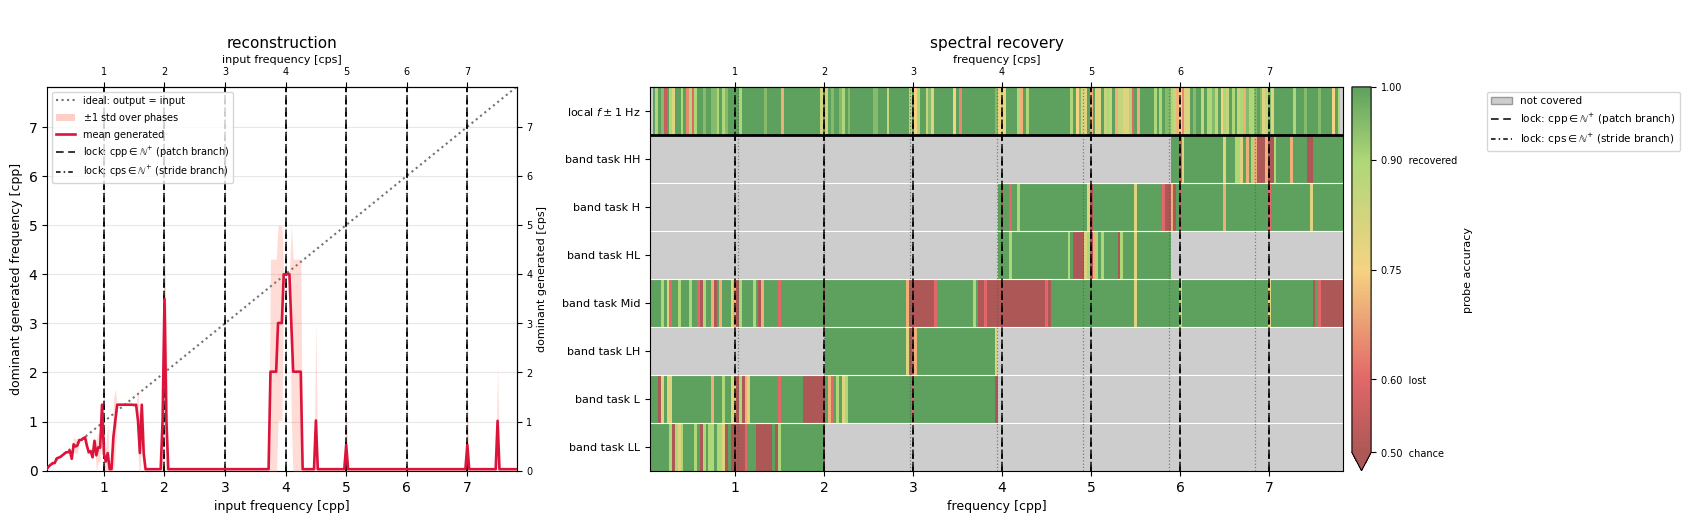
\includegraphics[width=\textwidth]{figures/fig_rec_16_16.png}
\caption{Behavioural reconstruction (left) and representational recovery (right) for pure tones under the retrained reference geometry $P=S=16$ and seed~42, with every frequency in cycles per patch (bottom and left) and cycles per stride (top and right). The left panel compares input and dominant generated frequencies, averaged over up to four starting phases with $\pm1$ standard deviation shaded; the right reports the accuracy of the local and hierarchical band probes. Dashed verticals mark the patch-branch sites ($\mathrm{cpp}\in\mathbb N^{+}$), which coincide with the stride-branch sites at $P=S$, and grey cells denote frequencies outside a task's coverage.}
    \label{fig:rec16-16}
\end{figure}

\subsection{Recovering a component from a complex background}

Tones added to a Light TSMixup or KernelSynth background are seldom returned by the retrained models, and over a large sample of draws the result was unexpected: the injected tone is much harder to recover at the control frequencies than at the candidate sites, reappearing in about a quarter of the trials on a site and almost never beside one, and still in a sixth to a fifth once the lines a forecast draws there with no tone added are discounted (\autoref{tab:decomposition}; procedure and single draws in \autoref{sec:appDecomp}). The pattern is the same for both generators, with the smallest patch retaining the most and the widest the least, which suggests that it belongs to the geometry rather than to the signal family, and the published checkpoint, which shares the reference geometry, returns added components more often on and off the sites. The result runs against the loss at the sites that $H1$ predicts and agrees with the attraction towards the sites seen in the sweep, and two mechanisms may contribute to it: a tone on a candidate site produces a repeating token sequence (\autoref{sec:tokenisation}) that a forecaster can prolong without representing the frequency, and the forecasts carry lines of their own on the candidate sites, which a count of presence credits as recovered and which account for between a quarter and two fifths of the lock recoveries. Whether a loss concentrates at the sites once background and phase are matched is what the Bayesian analysis was designed to decide.

\begin{table}[!tbp]
    \centering
    \small
    \setlength{\tabcolsep}{4.5pt}
    \renewcommand{\arraystretch}{1.15}
    \begin{tabular}{@{}cccccccc@{}}
        \toprule
        & & \multicolumn{3}{c}{\textbf{Light TSMixup}} & \multicolumn{3}{c}{\textbf{KernelSynth}} \\
        \cmidrule(lr){3-5} \cmidrule(l){6-8}
        \textbf{$P$} & \textbf{$S$} & \textbf{Lock} & \textbf{Net} & \textbf{Control} & \textbf{Lock} & \textbf{Net} & \textbf{Control} \\
        \midrule
        $16$ & $16^{\dagger}$ & $42$ & $33$ & $16$ & $43$ & $33$ & $16$ \\
        \midrule
        $8$ & $8$ & $53$ & $26$ & $0$ & $58$ & $39$ & $0$ \\
        \midrule
        $16$ & $8$ & $26$ & $14$ & $2$ & $25$ & $17$ & $3$ \\
        $16$ & $12$ & $35$ & $22$ & $1$ & $30$ & $23$ & $0$ \\
        $16$ & $16$ & $23$ & $6$ & $1$ & $22$ & $13$ & $0$ \\
        \midrule
        $24$ & $8$ & $36$ & $24$ & $1$ & $34$ & $32$ & $0$ \\
        $24$ & $12$ & $39$ & $28$ & $4$ & $35$ & $29$ & $4$ \\
        $24$ & $16$ & $25$ & $13$ & $0$ & $24$ & $20$ & $0$ \\
        $24$ & $20$ & $16$ & $10$ & $0$ & $16$ & $12$ & $1$ \\
        $24$ & $24$ & $40$ & $30$ & $2$ & $35$ & $27$ & $1$ \\
        \midrule
        $32$ & $8$ & $16$ & $14$ & $3$ & $15$ & $14$ & $3$ \\
        $32$ & $12$ & $18$ & $10$ & $1$ & $19$ & $15$ & $1$ \\
        $32$ & $16$ & $17$ & $9$ & $2$ & $13$ & $7$ & $4$ \\
        $32$ & $20$ & $6$ & $5$ & $4$ & $5$ & $5$ & $2$ \\
        $32$ & $24$ & $25$ & $22$ & $5$ & $25$ & $20$ & $4$ \\
        $32$ & $32$ & $13$ & $8$ & $6$ & $17$ & $15$ & $7$ \\
        \midrule
        \multicolumn{2}{c}{\textbf{Retrained mean}} & $25.9$ & $16.1$ & $2.1$ & $24.9$ & $19.2$ & $2.0$ \\
        \bottomrule
    \end{tabular}
\caption{Percentage of $100$ trials in which an added tone is recovered from the $64$-sample median forecast, at a candidate site (Lock) or at a nearby control (Control) on the same background and phase; a tone is recovered when a forecast line lies within $\pm1$\,Hz of it. Net credits a lock trial only if the forecast without the tone has no line there.\newline
$\dagger$ marks the published Chronos-Bolt-Tiny checkpoint.}
    \label{tab:decomposition}
\end{table}


\subsection{Prediction on the measured series}

On the photovoltaic series every checkpoint forecasts the same windows spread across the year and is scored on the same minutes (\autoref{tab:solarPrediction}; procedure in \autoref{sec:appSolar}). The error is concentrated in daylight and in the transitions around sunrise and sunset, whereas at night almost every model correctly continues a series held at zero, and the forecasts examined prolong the level of the last hour while the measured power has already begun to change. The published checkpoint is the most accurate, more plausibly because of its training than of its geometry; among the retrained models none improves on the $P=S=16$ baseline, several cannot be told apart from it and the rest are worse, with no ordering by overlap or by patch size; p32-s20 has the largest mean absolute error of all.

\begin{table}[!tbp]
    \centering
    \small
    \setlength{\tabcolsep}{4.5pt}
    \renewcommand{\arraystretch}{1.1}
    \begin{tabular}{@{}cccccccccc@{}}
        \toprule
        & & \multicolumn{3}{c}{\textbf{All minutes}} & \multicolumn{3}{c}{\textbf{MAE by regime}} & \multicolumn{2}{c}{\textbf{$\Delta$MAE vs retrained p16-s16}} \\
        \cmidrule(lr){3-5} \cmidrule(lr){6-8} \cmidrule(l){9-10}
        \textbf{$P$} & \textbf{$S$} & \textbf{MAE} & \textbf{Bias} & \textbf{RMSE} & \textbf{Night} & \textbf{Trans.} & \textbf{Day} & \textbf{Estimate} & \textbf{Interval} \\
        \midrule
        $16$ & $16^{\dagger}$ & $7.95$ & $-0.73$ & $19.12$ & $0.36$ & $11.25$ & $17.30$ & $-2.52$ & $[-3.63,\,-1.40]$ \\
        \midrule
        $8$ & $8$ & $11.11$ & $-4.05$ & $22.59$ & $1.53$ & $16.23$ & $22.69$ & $+0.64$ & $[-0.36,\,1.67]$ \\
        \midrule
        $16$ & $8$ & $9.86$ & $-1.57$ & $21.74$ & $1.41$ & $16.42$ & $19.61$ & $-0.61$ & $[-1.61,\,0.43]$ \\
        $16$ & $12$ & $14.60$ & $-1.67$ & $28.26$ & $2.17$ & $24.69$ & $28.83$ & $+4.13$ & $[2.69,\,5.56]$ \\
        $16$ & $16$ & $10.47$ & $-0.75$ & $20.77$ & $2.42$ & $18.20$ & $19.41$ & --- & --- \\
        \midrule
        $24$ & $8$ & $13.03$ & $0.75$ & $24.55$ & $1.88$ & $22.64$ & $25.67$ & $+2.56$ & $[1.41,\,3.76]$ \\
        $24$ & $12$ & $11.11$ & $-0.78$ & $22.08$ & $2.16$ & $19.43$ & $21.11$ & $+0.64$ & $[-0.45,\,1.80]$ \\
        $24$ & $16$ & $14.39$ & $-8.21$ & $29.06$ & $1.01$ & $17.21$ & $31.56$ & $+3.92$ & $[2.05,\,5.85]$ \\
        $24$ & $20$ & $15.54$ & $-5.01$ & $28.91$ & $3.48$ & $21.10$ & $30.32$ & $+5.07$ & $[3.47,\,6.74]$ \\
        $24$ & $24$ & $11.24$ & $0.14$ & $22.87$ & $1.32$ & $17.11$ & $23.11$ & $+0.77$ & $[-0.48,\,2.14]$ \\
        \midrule
        $32$ & $8$ & $14.32$ & $-2.21$ & $25.49$ & $4.65$ & $21.48$ & $25.55$ & $+3.85$ & $[2.83,\,4.83]$ \\
        $32$ & $12$ & $12.67$ & $-7.24$ & $26.23$ & $1.39$ & $15.74$ & $26.98$ & $+2.20$ & $[0.69,\,3.61]$ \\
        $32$ & $16$ & $13.34$ & $-2.24$ & $24.72$ & $2.18$ & $20.68$ & $26.51$ & $+2.87$ & $[1.89,\,3.93]$ \\
        $32$ & $20$ & $32.54$ & $3.43$ & $51.22$ & $13.59$ & $40.50$ & $55.95$ & $+22.07$ & $[16.91,\,27.36]$ \\
        $32$ & $24$ & $13.24$ & $-1.50$ & $26.62$ & $2.02$ & $23.28$ & $25.86$ & $+2.77$ & $[1.67,\,3.90]$ \\
        $32$ & $32$ & $10.56$ & $-0.30$ & $21.95$ & $1.47$ & $18.08$ & $20.94$ & $+0.09$ & $[-0.62,\,0.85]$ \\
        \bottomrule
    \end{tabular}
\caption{Error of the median forecast on the measured photovoltaic series, in watts, over $150$ disjoint windows and $9{,}187$ scored minutes per model. MAE is the mean absolute error, bias the mean error, RMSE the root mean square error, and Trans.\ the sunrise and sunset regime. $\dagger$ marks the published Chronos-Bolt-Tiny checkpoint. $\Delta$MAE is positive when a model is worse, with a $95\%$ bootstrap interval that resamples whole weeks.}
    \label{tab:solarPrediction}
\end{table}


The series offers insight into the application domain rather than a test of the design, because the dominant content of every window is the daily cycle, far below the first candidate site at one cycle per patch, so no window carries appreciable energy on $\mathcal F_{\mathrm{lock}}$. For the application the direction is nonetheless clear: content at the candidate sites reaches this plant only through weather transients lasting a few minutes, and those are the events a confirmed loss at the sites would leave the forecaster least able to represent.



\subsection{Bayesian analysis}\label{sec:bayesResults}

\autoref{tab:bayesModels} pairs each claim with the model and the single estimand that decides it, and the readings below follow that order. For every claim, \autoref{tab:bayesGates} gives the convergence of the fits it reads, each gate as passed, failed or not applicable, and the condition that set the verdict, so that a claim reported as not reportable names what it failed.

\begin{table*}[!htbp]
    \centering
    \footnotesize
    \setlength{\tabcolsep}{2.6pt}
    \begin{tabular}{@{}llrrrcccccccll@{}}
        \toprule
        \textbf{Claim} & \textbf{Model} & $\max\hat R$ & \textbf{min ESS} & \textbf{Div.} & \textbf{Conv.} & \textbf{Recov.} & \textbf{PPC} & \textbf{Sens.} & \textbf{LOO} & \textbf{D2} & \textbf{Net} & \textbf{Verdict} & \textbf{Decided by} \\
        \midrule
        $H1$ behav. & A & 1.004 & 4637 & 0 & \checkmark & \textbf{fail} & \textbf{fail} & \checkmark & -- & -- & \checkmark & not reportable & PPC, Recov. \\
        $M1$ & A$'$ & 1.004 & 4490 & 0 & \checkmark & \textbf{fail} & \textbf{fail} & \checkmark & \checkmark & -- & \checkmark & not reportable & PPC, Recov. \\
        $H1$ repr. & B & 1.003 & 2724 & 0 & \checkmark & \textbf{fail} & \textbf{fail} & \checkmark & -- & -- & -- & not reportable & PPC, Recov. \\
        $H2$ & C & 1.004 & 2457 & 0 & \checkmark & \textbf{fail} & \textbf{fail} & \checkmark & -- & -- & -- & not reportable & PPC, Recov. \\
        $H3$ location & D1 & 1.002 & 4935 & 0 & \checkmark & \checkmark & \textbf{fail} & \checkmark & \checkmark & -- & -- & not reportable & PPC \\
        $H3a$ & D2 & 1.003 & 1751 & 0 & \checkmark & \checkmark & \textbf{fail} & \checkmark & -- & \checkmark & -- & not reportable & PPC \\
        $H3b$ & D2 & 1.002 & 3214 & 0 & \checkmark & \textbf{fail} & \textbf{fail} & \checkmark & -- & \textbf{fail} & -- & not identified & 0 of 10 sites \\
        \bottomrule
    \end{tabular}
\caption{Convergence and gates of every claim, with the worst values over its fits; ESS is the effective sample size and Div.\ the divergences. Recov.\ is parameter recovery, PPC the posterior predictive check, Sens.\ prior sensitivity, LOO the reliability of the leave-one-out comparison, D2 the agreement of the two Model~D2 readings and Net that of Model~A with its net refit; a dash marks a gate that does not apply.}
    \label{tab:bayesGates}
\end{table*}


\begin{table*}[!tbp]
    \centering
    \footnotesize
    \setlength{\tabcolsep}{4pt}
    \renewcommand{\arraystretch}{1.15}
    \begin{tabular}{@{}llrlccll@{}}
        \toprule
        \textbf{Claim} & \textbf{Estimand} & \textbf{Median} & \textbf{95\% CrI} & {\boldmath$P(\textbf{support})$} & {\boldmath$P(\textbf{refute})$} & \textbf{Pre-gate} & \textbf{Post-gate} \\
        \midrule
        \multirow{2}{*}{$H1$ behav.} & $e^{\bar\beta}$ & $1.35$ & $[1.25,\,1.45]$ & $0.00$ & $1.00$ & refuted & \multirow{2}{*}{not reportable} \\
        \cmidrule[0.1pt]{2-7}
        & \quad net of the background & $1.38$ & $[1.28,\,1.50]$ & $0.00$ & $1.00$ & refuted & \\
        \midrule
        \multirow{3}{*}{$M1$} & $\delta_O$ & $-0.13$ & $[-0.29,\,0.03]$ & $0.053$ & $0.947^{\ddagger}$ & inconclusive & \multirow{2}{*}{not reportable} \\
        \cmidrule[0.1pt]{2-7}
        & \quad net of the background & $-0.12$ & $[-0.28,\,0.05]$ & $0.07$ & $0.93$ & inconclusive & \\
        \cmidrule[0.1pt]{2-8}
        & $\delta_P$ (descriptive) & $-0.05$ & $[-0.26,\,0.16]$ & -- & -- & -- & -- \\
        \midrule
        $H1$ repr. & $e^{\theta_{\mathrm{lock}}}$ & $1.059$ & $[1.043,\,1.075]$ & $0.00$ & $1.00$ & refuted & not reportable \\
        \midrule
        $H2$ & $\sigma_\phi$ & $0.006$ & $[0.003,\,0.014]$ & $1.00$ & $0.00$ & supported & not reportable \\
        \midrule
        \multirow{4}{*}{$H3$ location} & $\theta_S$, Light TSMixup & $-0.26$ & $[-0.29,\,-0.23]$ & \multirow{2}{*}{$0.92^{\S}$} & \multirow{2}{*}{$1.00$} & \multirow{4}{*}{refuted} & \multirow{4}{*}{not reportable} \\
        \cmidrule[0.1pt]{2-4}
        & $\theta_P$, Light TSMixup & $-0.017$ & $[-0.041,\,0.007]$ & & & & \\
        \cmidrule[0.1pt]{2-6}
        & $\theta_S$, KernelSynth & $-0.38$ & $[-0.41,\,-0.34]$ & \multirow{2}{*}{$0.84^{\S}$} & \multirow{2}{*}{$1.00$} & & \\
        \cmidrule[0.1pt]{2-4}
        & $\theta_P$, KernelSynth & $-0.014$ & $[-0.040,\,0.013]$ & & & & \\
        \midrule
        $H3a$ & $\kappa_S$ & $1.000$ & $[0.990,\,1.011]$ & $1.00$ & $0.00$ & supported & not reportable \\
        \midrule
        $H3b$ & $\kappa_P$ (three detections)$^{\P}$ & $4.4$ & $[2.8,\,6.0]$ & $0.00$ & $1.00$ & refuted & not identified \\
        \bottomrule
    \end{tabular}
\caption{Posterior median and $95\%$ credible interval (CrI) of every estimand, the probabilities that its claim is supported and refuted, and the verdict before and after the gates, one per claim. The net rows refit Model~A on the recovery net of the background-only forecast. $^{\ddagger}$Both probabilities lie within $0.003$ of their cuts. $^{\S}$Joint probability that both coefficients are negative on that generator. $^{\P}$Only three replicate curves show a patch-branch site, against the ten required, so the pre-gate reading is set aside.}
    \label{tab:bayesEstimates}
\end{table*}


\begin{figure*}[!p]
    \centering
    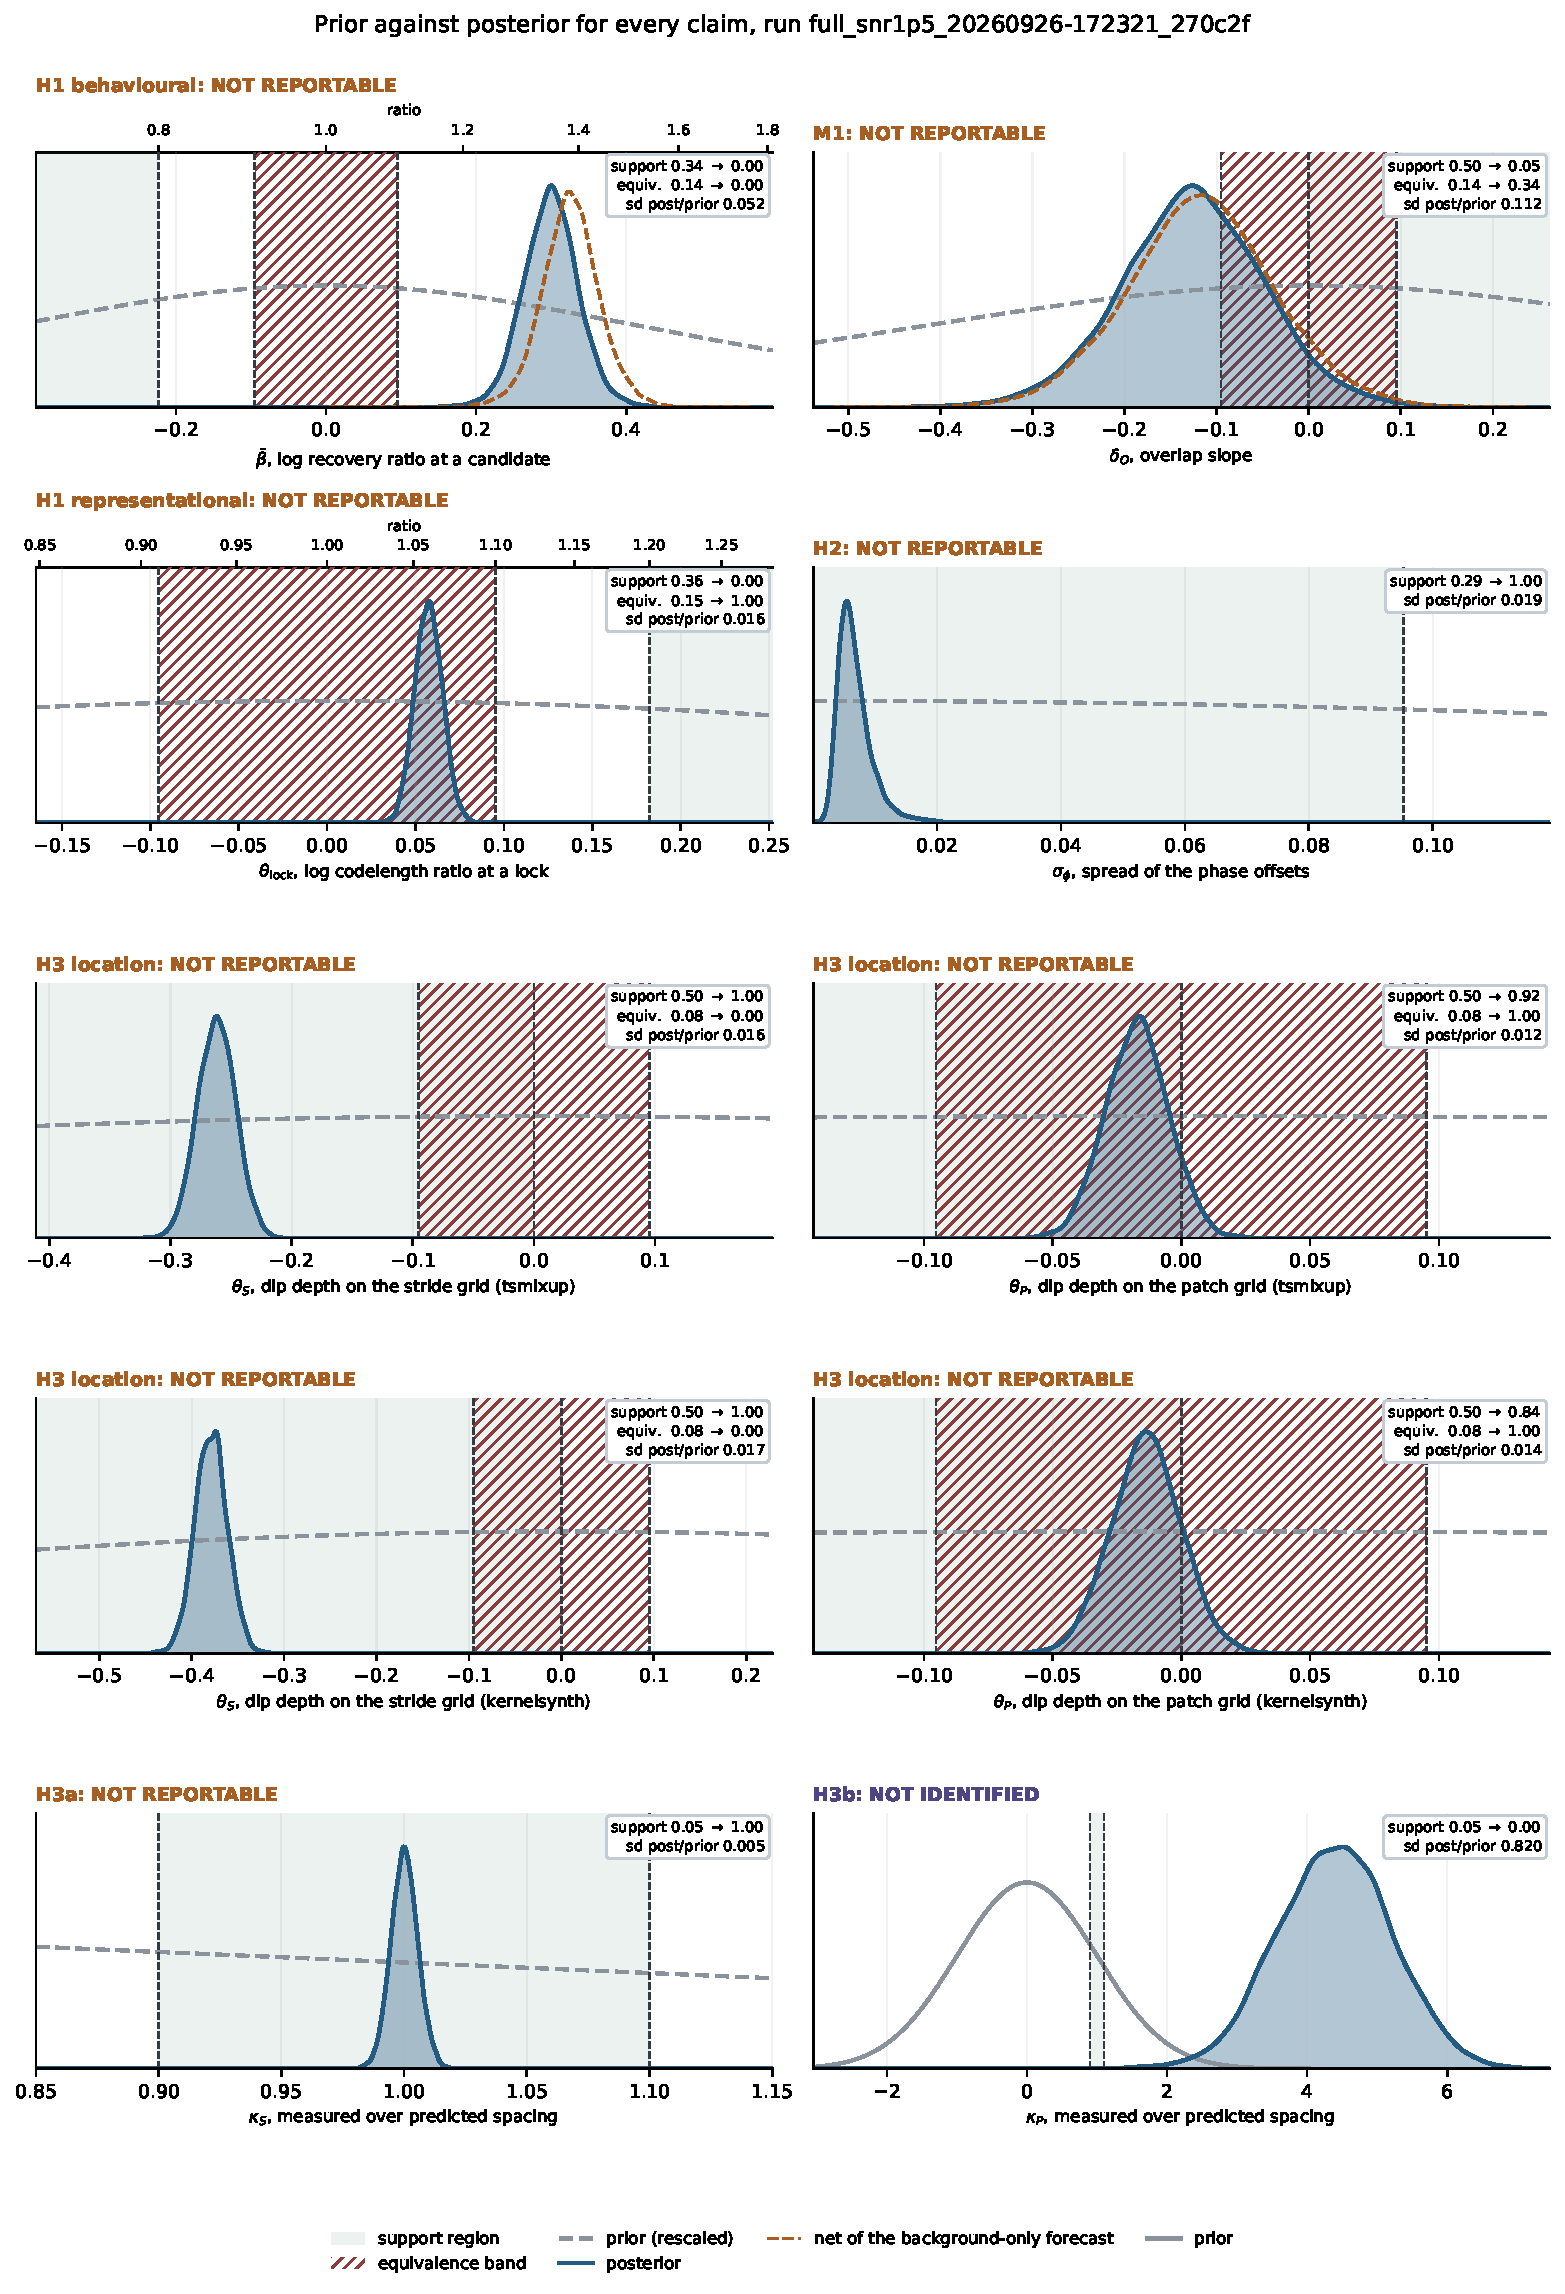
\includegraphics[width=\textwidth,height=0.88\textheight,keepaspectratio,trim={0 0 0 32},clip]{figures/bayes_prior_posterior.pdf}
\caption{Prior (grey) against posterior (blue) for the estimand of every claim, on the scale of its rule, with the support region shaded and the equivalence band hatched; each box gives the rule probabilities before and after the data. The dashed orange curve is Model~A net of the background-only forecast. Titles carry the verdict after the gates.}
    \label{fig:priorPosterior}
\end{figure*}

Every one of the $41$ fits converged, with $\hat R$ at most $1.004$, an effective sample size above $1700$ and no divergence, and no decision class moves over the prior-sensitivity ladder. Before the other gates the posteriors read clearly (\autoref{tab:bayesEstimates}, \autoref{fig:priorPosterior}). At a candidate frequency the forecast recovers more of the tone than at its controls, not less: $e^{\bar\beta}=1.35$ $[1.25,1.45]$, and $1.38$ once the lines the model draws with no tone are removed, so the rule of $H1$ on the forecast would refute it. The gain varies far more between candidate frequencies than between geometries, a scale of $1.2$ on the log ratio against $0.14$, as the attractors of the sweep suggested. In the internal state the codelength at a candidate grows by $6\%$ $[4,8]$, inside the $10\%$ equivalence band, which would refute $H1$ on the representation. The effect barely changes with phase, $\sigma_\phi=0.006$, which would support $H2$, although leave-one-out still detects a phase dependence too small to matter. The overlap slope is $\delta_O=-0.13$ $[-0.29,0.03]$, with $\Pr(\delta_O>0)=0.053$, and leave-one-out prefers the model without it, so $M1$ would be inconclusive at the edge of refutation; the patch-size slope, $\delta_P=-0.05$ $[-0.26,0.16]$, is not resolved, since recovery shows that this design cannot tell a slope of $-0.15$ from none. The token dispersion dips on the stride grid, $\theta_S=-0.26$ and $-0.38$ on the two generators, and not on the patch grid, $|\theta_P|<0.02$, as expected where the arithmetic makes consecutive patches identical only on the stride comb, so $H3$ location, which needs both, would be refuted, while the stride sites move exactly as predicted, $\kappa_S=1.000$ $[0.990,1.011]$, which would support $H3a$; no patch-only site was unambiguous, and $H3b$ is not identified. \autoref{fig:priorPosterior} shows every posterior far narrower than its prior and moved well away from it, so these readings are set by the data rather than by the priors; only $\delta_O$ straddles the boundary of its rule.

These readings are not verdicts, because each rests on conditions the gates test. Convergence establishes that the chains explored the posterior they report. Parameter recovery shows that a model, on this design, finds a known effect and returns a null when none is present, so that a null describes the data rather than a design unable to see an effect. The posterior predictive check asks whether the fitted model reproduces the data, stratum by stratum, since an estimand is only as credible as the model that defines it. Prior sensitivity shows that a conclusion belongs to the data rather than to the prior scale, the reliability gate shows that the comparisons behind $M1$ and $H3$ location rest on stable importance weights, and the agreement gates show that no conclusion depends on which of two defensible readings is used.

Convergence and sensitivity hold for every claim, and agreement wherever both readings exist; the predictive check fails for all of them, and recovery for Models~A, B and~C and for the patch branch of D2, so no claim is reportable and $H3b$ is not identified (\autoref{tab:bayesGates}). The models place the stratum means the estimands summarise close to the data, typically within $4\%$ of a stratum's standard deviation, but not its dispersion (\autoref{fig:ppcDispersion}): Model~A has one residual scale for fifteen geometries whose standard deviation ranges from $0.6$ to $1.8$, and a Student-$t$ likelihood cannot reproduce the skew of a contrast whose mean is $0.32$ and median $0.02$, while $371{,}000$ triplets make the replicated intervals narrow enough for any such mismatch to fail. The recovery failures are narrower, and \autoref{sec:appBayes} gives each. Reading the estimates as verdicts would assume the adequacy the gates were placed to test, so they remain the direction of the evidence rather than a decision on it.


\section{Discussion}\label{sec:discussion}
This section reads the Bayesian results claim by claim, evaluates the pre-registered mitigation and collects the limits of the evidence.

\subsection{Reading the Claims}\label{sec:claims}
All fits converged and no conclusion depends on its prior, so each posterior is a stable description of the data; what the gates withhold is the step from description to verdict. Two gates fail: the predictive check, when a model reproduces the average of a stratum but not its spread, and parameter recovery, when the design cannot find an effect of known size; one claim stops before them, because too few sites exist to identify its slope. Each claim below reports what its posterior shows before the gates and which gates then fail.

\subsubsection*{Frequency-dependent blind spots (H1)}
A tone at a candidate frequency is recovered $35\%$ better than beside it, and the probe needs only $6\%$ more code to read it from the internal state, so both readings would refute $H1$. No blind spot is visible, in line with the sites attracting the forecast in the sweep. Both models converged, yet neither is reportable. The predictive check fails on spread and not on location, since in Model~A one residual scale serves fifteen geometries whose spread differs threefold and the contrast is skewed beyond what a Student-$t$ likelihood reproduces. Recovery fails through a patch-size slope that the design cannot tell from none in Model~A, and by $0.003$ on one interval in Model~B.

\subsubsection*{Independence from temporal alignment (H2)}
Whatever advantage a candidate carries is nearly the same at every starting phase, so $H2$ would be supported. Model~C converged but, sharing its triplets with Model~A, fails the same predictive check, and its recovery fails through a single divergent repeat.

\subsubsection*{Parametric dependence of blind spot sites (H3)}
The geometry leaves a visible footprint in the token sequences, though not a loss. Their dispersion dips on the stride grid and not on the patch grid, so $H3$ location, which needs both, would be refuted, while the stride sites move as $f_s/S$ predicts and $H3a$ would be supported. $H3b$ cannot be examined: no patch-only site is unambiguous on the averaged curves, against the ten required, and three single replicates show one, so it is not identified rather than refuted. The fits converged and the stride results fail only the predictive check, on dispersion within each geometry, which sites on the predicted spacing leave without scatter to reproduce; the patch branch also fails recovery, its simulated refits diverging on three observations. Dips that follow from repeating tokens locate structure the geometry imposes and do not by themselves evidence a learned loss.

\subsubsection*{A candidate mitigation (M1)}
More overlap goes with a smaller gain at the sites and not with a smaller loss, so the data show no benefit of the mitigation. The fits converged and the leave-one-out comparison is reliable, but the rule fails on both legs before the gates and the claim then fails the predictive and recovery gates of Model~A, from which it is read.

\subsection{Mitigation: Evaluation and Further Strategies}\label{sec:mitigationDiscussion}
\begingroup
\let\subsection\subsubsection%
\subsection*{Evaluation of $M1$}

The overlap slope is $\delta_O=-0.13$, and $-0.12$ on the recovery net of the background-only forecast. Both legs of the rule fail: $\Pr(\delta_O>0\mid D)=0.053$ against $0.95$, and leave-one-out prefers the model without the overlap term by $0.7$ units of expected log predictive density against a paired standard error of $0.15$. The refutation probability, $0.947$, stops just short of its cut, so the reading is inconclusive before the gates and not reportable after them. Three confounds qualify any slope on this design. The token count moves with the stride, so overlap is not separated from sequence length; lowering $S$ changes the mix of stride and patch candidates; and the truncated context tail is non-zero on the six geometries that identify the stride branch.

\subsection*{Further strategies}

Because the candidate set follows from $(f_s,P,S)$ alone, the same arithmetic suggests two further strategies, neither tested here.

The first moves the combs rather than thinning one. Changing $S$ or $P$ rescales the corresponding comb by a known amount, so a deployment that knows its spectral content can choose a geometry whose combs fall between the components that matter. It is a design-time control rather than a repair, and it protects only the content known in advance.

The second is redundancy across geometries. Two models whose combs fall at different frequencies would be blind, if at all, in different places, and an ensemble switching per frequency on the observability assessment of \autoref{sec:ontology} would leave no frequency served only by a model known to be blind there. The cost is two forecasters to calibrate against each other and a switch that can itself be wrong.

$M1$ thins one branch, geometry selection moves both, and only redundancy covers what a single tokeniser cannot represent.
\endgroup

\subsection{Limitations}\label{sec:limitations}
Each geometry is one trained model from one seed, so a difference between two configurations is also a difference between two training runs, and the retrained models see a sixteenth of the published training windows (\autoref{sec:appRetraining}), which makes them comparable with one another but not with the released checkpoint. The mitigation slope carries the three confounds of \autoref{sec:mitigationDiscussion}, the truncated context among them (\autoref{tab:sweepContext}). The $64$-sample horizon resolves frequencies only to one bin, $f_s/64$, so a recovered line is located near a tone rather than resolved from its neighbours. The measured series carries no appreciable energy on $\mathcal F_{\mathrm{lock}}$, so the domain informs the risk reading but tests no hypothesis. Finally, Pagani et al\@. report frequency content recovered unevenly from Chronos representations. The pre-gate readings agree that the candidate sites are special, but not on the direction: the forecast recovers more there and the internal state loses under $10\%$, so, were the gates met, the unevenness would not be a loss concentrated on $\mathcal F_{\mathrm{lock}}$.


\section{Security Risk Assessment}\label{sec:security}
This section reads the phenomenon as a security risk under the Artificial Intelligence Risk Management Framework (AI RMF) of the National Institute of Standards and Technology (NIST).

The forecaster sits in a control loop in which its output drives battery dispatch and curtailment on a photovoltaic micro-grid, so a forecasting failure can become a control failure, and the property tested here is a security property as well as an accuracy one.

Phase-locking is deterministic, attacker-independent and present at deployment time, and the candidate set follows from $(f_s,P,S)$ alone, marking where a blind spot is most expected without excluding others. Where an exposure would sit, and how it moves with the configuration, is known before anything is measured: enough to place a monitor and to bound what a mitigation could reach, not enough to claim that a loss occurs.

\subsection{Risk Management Framework}
The AI RMF\autocite{tabassiArtificialIntelligenceRisk2023} is the reference for that reading. It separates the trustworthiness characteristics at stake, validity and reliability, security and resilience, from the governance functions that turn evidence into a control, and asks that known limitations be mapped, measured and managed rather than merely disclosed.

Its four functions assign responsibility and oversight (GOVERN), fix the deployment context and the pathways to harm (MAP), track the likelihood, severity and uncertainty of each risk (MEASURE), and select and monitor responses (MANAGE). They inform one another continuously, so \autoref{tab:riskRegister} records the functions each threat engages rather than a sequence.

None of the evidence each pathway needs establishes a loss (\autoref{tab:bayesEstimates}): before the gates the forecast recovers a tone better at a candidate than beside it, the representational cost lies within the equivalence band, and the stride sites sit where $f_s/S$ predicts. Every reading fails the gates, so the register records them as the direction of the evidence, lowers no residual on their strength, and keeps open every pathway that depends on a loss.

Each row of \autoref{tab:riskRegister} names a pathway, the functions it engages, the estimand that would establish it, the available control and the residual exposure, which stays conditional until that estimand passes the gates.

\begin{table*}[p]
    \centering
\small
    \setlength{\tabcolsep}{4.5pt}
    \begin{tabular*}{\textwidth}{@{\extracolsep{\fill}}>{\raggedright\arraybackslash}m{0.45cm}>{\raggedright\arraybackslash}m{3.35cm}>{\raggedright\arraybackslash}m{1.70cm}>{\raggedright\arraybackslash}m{3.85cm}>{\raggedright\arraybackslash}m{3.25cm}>{\centering\arraybackslash}m{1.45cm}@{}}
        \toprule
        \textbf{ID} & \textbf{Risk} & \textbf{AI RMF} & \textbf{Evidence in this report} & \textbf{Control available} & \textbf{Residual} \\
        \midrule
        $T1$ & Adversarial masking:\newline a periodic component injected on a candidate frequency may be under-represented and escape forecast-residual detection & \shortstack[l]{MAP\\MEASURE} & Precondition is the support rule $e^{\theta_{\mathrm{lock}}}>1.2$ (Model~B) with the site locations of $\kappa_S$ (Model~D2); the pathway itself needs the paired recovery ratio of Model~A. Pre-gate: $e^{\theta_{\mathrm{lock}}}=1.06$, $e^{\bar\beta}=1.35$, a gain; not reportable & Spectral monitor on the raw stream, upstream of tokenisation, at the enumerated candidate set & high \\
        \cmidrule(lr){1-6}
        $T2$ & Systematic blind spot with no adversary:\newline a legitimate plant harmonic sits on a candidate frequency and may be persistently under-represented & \shortstack[l]{MAP\\MEASURE\\MANAGE} & Candidate set is closed-form in $(f_s,P,S)$ and needs no fit; the cost at those sites is decided by $e^{\theta_{\mathrm{lock}}}$. Pre-gate: $1.06$, inside the equivalence band; not reportable & Choose $(P,S)$ against the known spectral content of the plant; \valueof{PartiallyObservable} degradation & medium \\
        \cmidrule(lr){1-6}
        $T3$ & Configuration drift:\newline a change of sampling interval, patch size or checkpoint geometry silently relocates the candidate set & \shortstack[l]{GOVERN\\MAP} & $H3a$: relocation is predicted in closed form by $f_s/S$, and whether the sites follow it is decided by $\kappa_S$. Pre-gate: $\kappa_S=1.000$ $[0.990,1.011]$; not reportable. The residual rests on the closed-form set, not on this reading & Recompute the candidate set from the knowledge base at every configuration change & low \\
        \cmidrule(lr){1-6}
        $T4$ & False assurance: overlap is increased and treated as a fix & \shortstack[l]{GOVERN\\MANAGE} & $M1$ is decided by $\delta_O$ under a two-leg rule; pre-gate both legs fail, $\delta_O=-0.13$, inconclusive and not reportable. Independently of any fit, the patch branch is invariant to $S$ by construction & Do not credit overlap as a control; record the unestablished status in the model card & high \\
        \cmidrule(lr){1-6}
        $T5$ & Defence placed inside the blind spot: phase randomisation, or anomaly detection on forecast residuals & MANAGE & $H2$ is decided by $\sigma_\phi$ (Model~C): a deficit independent of phase makes randomising it useless. Pre-gate: $\sigma_\phi=0.006$; not reportable & Move detection upstream of tokenisation; treat residual-based detection as insufficient alone & medium \\
        \bottomrule
    \end{tabular*}
\caption{Risk register. AI RMF names the function of the framework\autocite{tabassiArtificialIntelligenceRisk2023} engaged by each item. Residual is the exposure left by the control, judged qualitatively: high where no operator control closes it, medium where the control is partial or needs design-time choices, low where a procedure that follows from the arithmetic closes it. No residual is lowered on estimates that fail the gates.}
    \label{tab:riskRegister}
\end{table*}


\subsection{Adversarial-masking threat model}
A weakness becomes a vulnerability when someone can reach it. Because phase-locking is deterministic, an adversary needs no model access, query budget or knowledge of the training corpus, only the configuration $(f_s,P,S)$ of the deployed forecaster, from which $\mathcal F_{\mathrm{lock}}$ follows by arithmetic. In the taxonomy of adversarial machine learning\autocite{vassilevAdversarialMachineLearning2024} the weakness is an availability violation, since what the model would lose at a candidate frequency would be lost for every input and user. It becomes an integrity violation of the evasion type once an adversary uses that loss to hide a manipulation.\footnote{Deliverable~2 classified the weakness as an availability violation only. The classification is extended because the masking threat model developed here seeks to hide a manipulation rather than to degrade the service, which the taxonomy treats as evasion.}

\autoref{tab:threatModel} sets out the adversarial-masking threat model in five elements, from the actor's capability and access path to the manipulation, the consequence and the exposure left after the mitigation. Every row is conditional: it describes the exposure that would follow if a loss at the candidate sites were confirmed, not one that has been observed.

\begin{table}[!t]
    \centering
\small
    \setlength{\tabcolsep}{5pt}
    \begin{tabular}{@{}M{0.215\linewidth} M{0.735\linewidth}@{}}
        \toprule
        \textbf{Element} & \textbf{Reading for this system} \\
        \midrule
        Adversary capabilities & No model access of any kind and no knowledge of the training corpus, only knowledge of the configuration $(f_s,P,S)$ and the ability to drive a periodic load on the photovoltaic plant, which an inverter switching schedule or a switchable load already provides. \\
        \addlinespace[3pt]
        Attack surface & The raw telemetry stream before tokenisation, reached by acting on the physical process or on the data path. \\
        \addlinespace[3pt]
        Manipulation of telemetry & A small periodic component at a candidate frequency, which is legitimate plant behaviour and survives any plausibility check on the raw signal. \\
        \addlinespace[3pt]
        Operational consequence & The component is present in the plant and, if structural aliasing is confirmed, under-represented in the model, so dispatch and curtailment are decided on an incomplete picture, and a detector reading the forecast residual is looking through the same tokeniser that lost it. \\
        \addlinespace[3pt]
        Residual risk & The pre-registered mitigation raises overlap by shortening the stride at fixed patch size, so it thins the stride branch alone and $\mathcal{F}_{P}$ survives at every deployed configuration. Shrinking the patch instead thins $\mathcal{F}_{P}$, and with it $\mathcal{F}_{S}$ once $S \le P$ forces the stride down as well; but that raises both fundamentals rather than closing either comb, so the candidate set is relocated and thinned, not removed. \\
        \bottomrule
    \end{tabular}
\caption{The adversarial-masking threat model in five elements, from the capability the actor needs to the exposure left after the pre-registered mitigation. The first row sets it apart: what is required is not access to the model but the ability to make the plant do something it is entitled to do, so nothing in the manipulation is anomalous where a plausibility check would sit.}
    \label{tab:threatModel}
\end{table}


This is the adversarial-masking row of \autoref{tab:riskRegister}, carried at high residual: the injected component is legitimate plant behaviour, which a monitor on the raw stream can locate at a candidate frequency but cannot tell from ordinary operation.

\subsection{Threat models beyond the adversarial one}

The framework asks for systematic vulnerability, not only for attacks, and the more likely exposure has no adversary. On one-minute telemetry, \autoref{eq:branches} puts the patch branch of a $P{=}16$ tokeniser at periods of $16/k$ minutes: $16$, $8$, $5.3$, $4$, $3.2$, $2.7$ and $2.3$ minutes. These are the timescales of inverter duty cycling and cloud-shadow transients, ordinary plant behaviour sitting on the frequencies at which the model may be least able to represent it. If the loss were confirmed, a monitor built on such a forecaster would be systematically less sensitive there, for reasons no operational log would reveal. This is the systematic blind spot of \autoref{tab:riskRegister}, and the reason the candidate set belongs in the deployment documentation.

The third exposure, configuration drift, is a matter of governance. Because the candidate set is a function of configuration, changes that no one would route through a security review relocate it: resampling telemetry from one minute to thirty seconds, swapping to a checkpoint of another geometry, or choosing a patch size for latency. $H3a$ would make this tractable: if the sites follow $f_s/S$, recomputing the candidate set after a change is arithmetic rather than re-measurement.

\subsection{Controls and residual exposure}

Two controls in this design are real. The first answers the defence placed inside the blind spot ($T5$ in \autoref{tab:riskRegister}): detection has to sit before tokenisation, on the raw telemetry, since anything placed after it would inherit any blind spot the tokeniser induces. A spectral monitor on the raw stream is inexpensive because the candidate set is closed-form. The second is the semantic layer of \autoref{sec:appOntology}, which degrades actuation rather than failing silently: a \valueof{PartiallyObservable} assessment reduces the battery cap and lowers decision confidence, so uncertainty about the representation reaches the actuator instead of being resolved by assumption. This is the resilience the framework asks for, and it does not depend on how the behavioural claim resolves.

One control cannot be credited. The pre-registered mitigation, increased patch overlap, is not established: both legs of its rule fail and the reading is not reportable. Even if established it would be partial, since overlap moves the stride branch and leaves the patch branch untouched. An operator who raises the overlap and records the risk as mitigated has bought the false assurance of \autoref{tab:riskRegister}, which is why it is carried at high residual.


% The Conclusions open a page: the last page of the Security Risk Assessment ends at its natural height
% instead of being stretched to the full one.
\newpage
\section{Conclusions}\label{sec:conclusions}
This report asked whether a patch-based forecaster preserves the frequency content of signals that classical sampling theory says are fully representable, and how $f_s$, $P$ and $S$ decide when it does not. The characterisation is complete and depends on no fit. A tone completing a whole number of cycles in one stride repeats its tokens; one completing a whole number in one patch repeats their content; and the union of the two combs is a closed-form candidate set computable for a geometry never measured. That set locates where a loss could sit, not that one exists, and the report holds the two apart throughout.

Whether a trained model does lose information there remains open, and the design that decides it is fixed in advance: it returns not reportable or not identified rather than a null when a fit fails to earn a verdict. Two consequences already follow: patch geometry is a deployment parameter to be chosen against the known spectral content of a plant, not a default to inherit; and since a detector placed after tokenisation would inherit any blind spot there, monitoring must act on the raw signal upstream. Neither waits on the fits, and neither is available to a system that treats the tokeniser as opaque.

The exploratory steps agree: added tones are recovered more often on the sites than beside them, and on the photovoltaic series no retrained geometry beats the $P=S=16$ baseline, with no appreciable energy at the sites. The Bayesian analysis returned a direction but no verdict. Before the gates, the rules would refute $H1$ on both readings: at a candidate frequency the forecast recovers the tone $35\%$ better than beside it, and the internal state needs only $6\%$ more code to read it. They would support $H2$, the effect barely changing with phase, and $H3a$, the stride sites moving exactly as $f_s/S$ predicts; the patch-grid dip lies inside its equivalence band, so $H3$ location would be refuted, $M1$ would be inconclusive and $H3b$ is not identified. Every model converged and none depends on its prior, but none reproduces the dispersion of the data and Models~A to~C and the patch branch of D2 also fail parameter recovery, so under the rules fixed in advance every claim is not reportable. For the security reading this removes no exposure and establishes none: the sites are real, predictable and treated differently by the model, which is what an operator needs to monitor them, and the direction of the evidence is that they attract the forecast rather than blind it. Until a claim is reportable, the agent of \autoref{sec:agent} keeps every candidate frequency \valueof{PartiallyObservable} and acts in \valueof{ConservativeMode}.

If confirmed, structural aliasing in a patch-based forecaster would be a configuration-determined, attacker-independent weakness whose candidate sites are derivable in closed form rather than conjectured. What the arithmetic settles on its own is that most sites exclusive to one branch lie on the patch branch (\autoref{tab:branchSites}), that the pre-registered mitigation cannot reach that branch whatever the fit returns, and that any exposure there cannot be managed by overlap inside the model. It has to be managed around the model, with the candidate set recomputed whenever the configuration changes.

Four extensions would sharpen the claim. The first is the one every verdict now waits on: models that reproduce the dispersion of the contrast, with a residual scale per geometry and a skewed likelihood. The others are independently trained instances per geometry, which a single seed cannot separate from geometry, an untrained-network baseline on the same dispersion measurement, and a test of whether a candidate set derived at $512$\,Hz survives translation to telemetry sampled once a minute.


\flushfloatpages
\printbibliography[]

\setcounter{secnumdepth}{0} % appendices and their subdivisions stay unnumbered

\flushfloatpages
\appendixsection{Ontology of the Photovoltaic Application Domain}{sec:appOntology}
\begingroup \let\section\subsection \let\subsection\subsubsection
This appendix defines a compact ontology for a photovoltaic (PV) system governed by one control agent, based on the data provided by SolarTech Lab \autocite{levaPhotovoltaicPowerWeather2020}. It connects environmental and electrical observations to anomaly recognition, Chronos-style patched representations, structural-aliasing evidence, and bounded power-routing decisions \autocite{ansariChronosLearningLanguage2024}. Power-routing is included only as the operational endpoint of the semantic model; the principal concern remains whether the representation preserves the information on which the agent relies.

\section{Domain Description}

The modelled system contains four energy assets: a photovoltaic array, battery storage, an aggregate internal load, and an external grid. The internal load is a passive sink representing a factory or a fleet of machines. Its demand is observed, but it has no agent, machine-level taxonomy, curtailment command, or scheduling model. The external grid is an available bidirectional boundary bus which supplies residual demand and accepts residual production.

Exactly one \pv{ControlAgent} coordinates the four passive assets: it observes one synchronised control cycle, assigns environmental, anomaly, and observability states, selects a control mode, and emits one or more directional decisions, with no peer-to-peer negotiation among assets.

The seven admissible transfer directions are
\begin{equation}
\label{eq:routes}
\begin{aligned}
\mathrm{PV}&\rightarrow\mathrm{Load}, &
\mathrm{PV}&\rightarrow\mathrm{Battery}, &
\mathrm{PV}&\rightarrow\mathrm{Grid},\\
\mathrm{Battery}&\rightarrow\mathrm{Load}, &
\mathrm{Battery}&\rightarrow\mathrm{Grid}, &
\mathrm{Grid}&\rightarrow\mathrm{Load},\\
&&\mathrm{Grid}&\rightarrow\mathrm{Battery}.&&
\end{aligned}
\end{equation}
They satisfy the cycle-level balance
\begin{equation}
\label{eq:power-balance}
P_{\mathrm{pv}}+P_{\mathrm{bat,dis}}+P_{\mathrm{grid,in}}
=P_{\mathrm{load}}+P_{\mathrm{bat,ch}}+P_{\mathrm{grid,out}}.
\end{equation}
All terms denote non-negative magnitudes; import and export are therefore kept separate rather than encoded by an ambiguous sign.

\section{Purpose and Scope}

The ontology provides the smallest semantic layer needed to represent the physical boundary, validated observations, environmental context, three selected anomalies, and the effect of the tokenisation over model observability. It does not model individual machines, market prices, dispatch optimisation, grid faults, or a deployed real-time controller. Load demand, battery state of charge (SoC), asset limits, and the optional grid-exchange reference are asserted because they are not present in the photovoltaic telemetry dataset.

The environmental states are operational generation proxies, not meteorological diagnoses, and likewise the routing rules describe a deterministic conceptual policy rather than the central experimental contribution. Structural aliasing remains an empirically tested property of a signal-representation pair.

\section{Ontology Representation}

\subsection{Core classes and closed vocabularies}

\autoref{tab:classes} defines the compact class interface: the four asset subclasses form a disjoint union; the \pv{PVSystem} contains exactly one asset of each type and it is managed by a control agent. Reading down its rows shows the design decision the rest of the appendix rests on: the physical plant, the observation, the model configuration and the assessment are separate classes rather than attributes of one another, so a tokenisation geometry is an object the reasoner can quantify over instead of a parameter buried in a checkpoint.

\begin{table}[!tbp]
\centering
\small
\begin{tabular}{@{}M{0.29\linewidth}M{0.64\linewidth}@{}}
\toprule
\textbf{Class} & \textbf{Role} \\
\midrule
\pv{PVSystem} & Aggregate system and scope of each control cycle. \\
\rowsep
\pv{EnergyAsset} & Parent of the four passive physical assets. \\
\rowsep
\pv{PhotovoltaicArray} & Intermittent renewable source measured through PV telemetry. \\
\rowsep
\pv{BatteryStorage} & Bounded storage asset that can charge, discharge, or hold. \\
\rowsep
\pv{InternalLoad} & Aggregate passive demand of a factory or machine fleet. \\
\rowsep
\pv{ExternalGrid} & Reliable bidirectional boundary bus for residual balancing. \\
\midrule
\pv{ControlAgent} & The single decision-making entity. \\
\rowsep
\pv{SystemObservation} & Time-stamped snapshot of PV, environment, battery, load, and grid reference. \\
\midrule
\pv{TimeSeriesSignal} & Physical signal and its temporal descriptors. \\
\rowsep
\pv{PatchedRepresentation} & A model input representation defined by patch and stride. \\
\rowsep
\pv{Forecast} & Horizon of predicted values produced from a \pv{PatchedRepresentation} and consumed by the \pv{ControlAgent}. \\
\rowsep
\pv{ObservabilityAssessment} & Evidence linking a signal-representation pair to an observability state. \\
\midrule
\pv{GenerationContext} & Operational proxy for expected solar generation. \\
\rowsep
\pv{AnomalyState} & Detected physical or sensing abnormality. \\
\rowsep
\pv{ObservabilityState} & Semantic assessment of information retained after patching. \\
\rowsep
\pv{ControlMode} & Normal, conservative, or safe operating policy. \\
\rowsep
\pv{PowerRoute} & Closed vocabulary of the seven admissible source--destination pairs. \\
\midrule
\pv{PowerRoutingDecision} & One directional transfer or hold decision with an optional bounded setpoint. \\
\bottomrule
\end{tabular}
\caption{Core classes in the simplified ontology.}
\label{tab:classes}
\end{table}


Five closed vocabularies complete the interface. The generation context takes the values \valueof{ClearSky}, \valueof{PartialCloud}, \valueof{Overcast} and \valueof{Nighttime}; the anomaly state \valueof{InverterTrip}, \valueof{RampEvent} and \valueof{SensorMalfunction}; the observability state \valueof{Observable}, \valueof{PartiallyObservable} and \valueof{StructurallyAliased}; and the control mode \valueof{NormalMode}, \valueof{ConservativeMode} and \valueof{SafeMode}. The power route names the seven admissible transfers: \valueof{PVToInternalLoad}, \valueof{PVToBattery} and \valueof{PVToExternalGrid} from the array, \valueof{BatteryToInternalLoad} and \valueof{BatteryToExternalGrid} from the battery, and \valueof{ExternalGridToInternalLoad} and \valueof{ExternalGridToBattery} from the grid.

Formally, each vocabulary class is an OWL-style enumeration of the listed named individuals (\texttt{oneOf}). The five vocabulary classes are pairwise disjoint, and all listed values are declared globally different (\texttt{AllDifferent}). This prevents a value such as \valueof{SafeMode} from being silently identified with \valueof{ClearSky} or \valueof{NormalMode} under open-world semantics. Each valid time-stamped observation has exactly one generation context, each completed observability assessment has exactly one observability state, and each routing decision records exactly one control mode. Co-issued decisions based on the same synchronised observation must record the same mode. Anomalies are not declared mutually exclusive because, for example, an abrupt inverter trip also creates a large power change.

\subsection{Object properties}

The semantic relations in \autoref{tab:objects} connect the physical boundary to the inference and control layers. Each active \pv{PowerRoutingDecision} has exactly one route value, one source, and one distinct destination. Its non-negative setpoint magnitude is optional because \texttt{Balance} may denote passive residual exchange.

\begin{table}[!tb]
\centering
\small
\begin{tabular}{@{}M{0.25\linewidth}M{0.29\linewidth}M{0.37\linewidth}@{}}
\toprule
\textbf{Property} & \textbf{Domain} & \textbf{Range or meaning} \\
\midrule
\pv{hasAsset} & \multirow{3}{=}{\pv{PVSystem}} & \pv{EnergyAsset} \\
\cmidrule[0.1pt]{1-1}\cmidrule[0.1pt]{3-3}
\pv{managedBy} &  & exactly one \pv{ControlAgent} \\
\cmidrule[0.1pt]{1-1}\cmidrule[0.1pt]{3-3}
\pv{hasObservation} &  & \pv{SystemObservation} \\
\rowsep%
\pv{hasSignal} & \pv{PhotovoltaicArray} & \pv{TimeSeriesSignal} \\
\midrule
\pv{hasGenerationContext} & \multirow{2}{=}{\pv{SystemObservation}} & zero or one \pv{GenerationContext} value \\
\cmidrule[0.1pt]{1-1}\cmidrule[0.1pt]{3-3}
\pv{hasAnomaly} &  & zero or more \pv{AnomalyState} values \\
\midrule
\pv{hasRepresentation} & \pv{TimeSeriesSignal} & \pv{PatchedRepresentation} \\
\rowsep%
\pv{forecastFrom} & \multirow{2}{=}{\pv{Forecast}} & exactly one \pv{PatchedRepresentation} \\
\cmidrule[0.1pt]{1-1}\cmidrule[0.1pt]{3-3}
\pv{informsAnomaly} &  & \pv{AnomalyState} \\
\rowsep%
\pv{assessesRepresentation} & \multirow{2}{=}{\pv{ObservabilityAssessment}} & exactly one \pv{PatchedRepresentation} \\
\cmidrule[0.1pt]{1-1}\cmidrule[0.1pt]{3-3}
\pv{hasObservabilityState} &  & one \pv{ObservabilityState} value \\
\midrule
\pv{makesDecision} & \pv{ControlAgent} & \pv{PowerRoutingDecision} \\
\rowsep%
\pv{selectsMode} & \multirow{5}{=}{\pv{PowerRoutingDecision}} & exactly one \pv{ControlMode} value \\
\cmidrule[0.1pt]{1-1}\cmidrule[0.1pt]{3-3}
\pv{basedOn} &  & observation, assessment, or inferred state \\
\cmidrule[0.1pt]{1-1}\cmidrule[0.1pt]{3-3}
\pv{hasRoute} &  & zero or one \pv{PowerRoute} value \\
\cmidrule[0.1pt]{1-1}\cmidrule[0.1pt]{3-3}
\pv{hasSourceAsset} &  & zero or one \pv{EnergyAsset} \\
\cmidrule[0.1pt]{1-1}\cmidrule[0.1pt]{3-3}
\pv{hasDestinationAsset} &  & zero or one \pv{EnergyAsset} \\
\bottomrule
\end{tabular}
\caption{Object-property signatures.}%
\label{tab:objects}
\end{table}


\pv{hasRepresentation} is intentionally non-functional because one signal can be evaluated under several $(P,S)$ configurations. Each assessment identifies exactly which representation it evaluates, and each decision is based on exactly one current observation and its completed assessment; its own \pv{selectsMode} value therefore scopes the mode without accumulating incompatible modes on the persistent agent. The range of \pv{basedOn} is the union of observation and inferred-assessment entities, rather than the intersection that multiple range declarations in RDF Schema (RDFS) would imply.

OWL's open-world semantics do not by themselves validate that endpoint types match a named route. The operational validator therefore admits only the seven ordered pairs in \autoref{eq:routes}, rejects identical endpoints, and checks consistency among \pv{hasRoute}, source, and destination. A hold decision has no route or endpoints and has a zero or absent setpoint.

\subsection{Data properties and units}

\autoref{tab:data} groups the quantitative data properties by owning class and encodes units in their names, so that the routing rules of \autoref{tab:routing}, which compare quantities across classes, remain verifiable. It separates measured environmental evidence, asserted or simulated plant state and the optional grid reference, and each control-critical entry carries its own validity flag, so a fall-back to safe mode can name the critical input that caused it, while the optional grid reference never blocks the controller.

The synchronised observation combines the measured photovoltaic and environmental variables with asserted or simulated battery, load, and grid-reference values. The control-critical quantities are PV power $P_{\mathrm{pv}}$, tilted irradiance $G_{\mathrm{tilt}}$, normalised battery state of charge $s\in[0,1]$, and aggregate load demand $P_{\mathrm{load}}\geq0$. Each has a separate validity flag derived from presence, finiteness, freshness, and a configured physical range. Horizontal irradiance, air temperature, wind speed, and wind direction remain environmental evidence but do not independently block the controller. The signed \pv{gridExchangeReferenceW} is optional, with positive values denoting export; it is usable only when present, finite, and fresh.

Missing or stale data cannot be inferred safely from OWL's open-world assumption alone. An operational validation layer therefore compares the observation time stamp with a configurable staleness limit, validates numeric ranges, and asserts the four critical Boolean flags consumed by the ontology, which keeps data-quality validation distinct from semantic classification.

\begin{table}[!tbp]
\centering
\small
\begin{tabular}{@{}M{0.29\linewidth}M{0.63\linewidth}@{}}
\toprule
\textbf{Owner} & \textbf{Data properties} \\
\midrule
\pv{SystemObservation} & \pv{pvPowerW}, \pv{powerRampRateWPerS}, \pv{loadDemandW}, optional \pv{gridExchangeReferenceW}, \pv{tiltedIrradianceWm2}, \pv{horizontalIrradianceWm2}, \pv{airTemperatureC}, \pv{windSpeedMs}, \pv{windDirectionDeg}, \pv{batterySoC}, \pv{observationTimestamp}, \pv{pvPowerValid}, \pv{tiltedIrradianceValid}, \pv{batterySoCValid}, and \pv{loadDemandValid}. \\
\rowsep%
\pv{BatteryStorage} & \pv{capacityWh}, \pv{reserveSoC}, \pv{targetSoC}, \pv{maximumSoC}, \pv{maximumChargePowerW}, and \pv{maximumDischargePowerW}. \\
\midrule
\pv{TimeSeriesSignal} & \pv{signalFrequencyHz}, \pv{samplingFrequencyHz}, \pv{periodSamples}, \pv{amplitudeW}, \pv{timeSpanSeconds}, and \pv{phaseOffsetSamples}. \\
\rowsep%
\pv{PatchedRepresentation} & \pv{patchSize}, \pv{stride}, and derived \pv{overlapRatio}. \\
\rowsep%
\pv{ObservabilityAssessment} & \pv{analysisStatus}, \pv{assessmentMethod}, \pv{assessmentMetric}, \pv{strideLockingRatio}, \pv{patchLockingRatio}, \pv{lockingTolerance}, \pv{effectEstimate}, \pv{posteriorLossProbability}, \pv{credibleIntervalLower}, \pv{credibleIntervalUpper}, and \pv{assessmentTimestamp}. \\
\midrule
\pv{PowerRoutingDecision} & optional non-negative \pv{powerSetpointW}, \pv{decisionConfidence}, \pv{batteryCommand} in \{Charge, Discharge, Hold\}, \pv{pvCommand} in \{Connect, Isolate\}, and \pv{gridCommand} in \{Import, Export, Balance\}. \\
\bottomrule
\end{tabular}
\caption{Quantitative property groups and units encoded by their names.}%
\label{tab:data}
\end{table}


A valid patched representation satisfies $P\geq1$ and $1\leq S\leq P$, and stores the overlap ratio $O$ of \autoref{eq:overlap} as descriptive metadata. It is not used as a standalone rule for declaring aliasing.

\section{Inference Rules}

\subsection{Environmental generation context}

Let $g_0<g_1<g_2$ be site-configurable tilted-irradiance thresholds and let $G_t$ denote the validated value of $G_{\mathrm{tilt}}$ at time $t$. The active generation context is
\begin{equation*}
Z_G(G_t)=
\begin{cases}
\valueof{Nighttime}, & G_t\leq g_0,\\
\valueof{Overcast}, & g_0<G_t<g_1,\\
\valueof{PartialCloud}, & g_1\leq G_t<g_2,\\
\valueof{ClearSky}, & G_t\geq g_2.
\end{cases}
\end{equation*}
Values $g_0=0$, $g_1=150$, and $g_2=800\ \mathrm{W\,m^{-2}}$ are retained only as an illustrative configuration compatible with the current coursework rather than as universal meteorological boundaries. Low irradiance can also be caused by solar position.

\subsection{Anomaly detection and precedence}

Let $v_P(t)$, $v_G(t)$, $v_s(t)$, and $v_L(t)$ denote the validity of PV power, tilted irradiance, battery SoC, and aggregate load demand. The control-critical validity predicate is
\begin{equation*}
V_t=v_P(t)\wedge v_G(t)\wedge v_s(t)\wedge v_L(t).
\end{equation*}
If $V_t$ is false, no physical anomaly or forecast-driven route is inferred from that observation. A valid irradiance value may still support a descriptive generation context, but the operational validator asserts \valueof{SensorMalfunction} and the cycle proceeds directly to safe-mode selection. Within a validated cycle, absence of the three listed anomaly values is interpreted locally as ``none detected''; this is a scoped closed-world policy, not a global OWL assumption. The signed ramp rate, measured in watts per second when $\Delta t$ is expressed in seconds, is
\begin{equation}
\label{eq:signed-ramp}
r_t=\frac{P_t-P_{t-1}}{\Delta t}.
\end{equation}
The anomaly rules are expressed with configurable thresholds: $g_{\mathrm{trip}}$ for sufficient irradiance, $p_0$ for positive near-zero power, and $r_{\max}$ for maximum admissible ramp magnitude. The controller evaluates sensor validity first, so a sensor malfunction cannot be reinterpreted as a physical ramp or inverter trip. If a valid inverter trip also satisfies the ramp predicate, the safe response to the trip takes precedence over ramp smoothing.

\subsubsection{Sensor malfunction}

\valueof{SensorMalfunction} is an evidence-quality condition, not a claim that the plant has failed: at least one control-critical measurement is absent, stale, non-finite or out of range (\autoref{eq:sensor-malfunction}).
\begin{equation}
\neg V_t \longrightarrow \valueof{SensorMalfunction}.
\label{eq:sensor-malfunction}
\end{equation}

\subsubsection{Inverter trip}

\valueof{InverterTrip} denotes a loss of photovoltaic conversion while irradiance is sufficient for non-negligible production. It is distinguished from naturally low output at night or under weak irradiance by requiring valid telemetry, $G_t\geq g_{\mathrm{trip}}$, and $|P_t|\leq p_0$ in \autoref{eq:inverter-trip}; its safe response isolates the photovoltaic side.
\begin{equation}
V_t\wedge G_t\geq g_{\mathrm{trip}}\wedge |P_t|\leq p_0
\longrightarrow \valueof{InverterTrip}.
\label{eq:inverter-trip}
\end{equation}

\subsubsection{Ramp event}

\valueof{RampEvent} denotes an abrupt change in photovoltaic power between two consecutive valid observations. Its magnitude is determined by the signed rate $r_t$ of \autoref{eq:signed-ramp} and must exceed the calibrated bound $r_{\max}$ in \autoref{eq:ramp-event}; the sign distinguishes a rapid production increase from a rapid decrease for the subsequent control response.
\begin{equation}
V_t\wedge V_{t-1}\wedge |r_t|>r_{\max}
\longrightarrow \valueof{RampEvent}.
\label{eq:ramp-event}
\end{equation}
No numerical value is inherited for $r_{\max}$ because it must be calibrated after invalid values and outliers have been excluded.

\subsection{Signal observability and structural aliasing}

For a signal frequency $f$, sampling frequency $f_s$, patch size $P$, and stride $S$, the ontology uses the cycles per stride and per patch of \autoref{sec:tokenisation},
\begin{equation*}
\mathrm{cps}=\frac{fS}{f_s},
\qquad
\mathrm{cpp}=\frac{fP}{f_s},
\end{equation*}
stored as the data properties \pv{strideLockingRatio} and \pv{patchLockingRatio}. A stride-lock candidate $L_S$ and a patch-aligned periodicity candidate $L_P$ are
\begin{equation}
\begin{aligned}
L_S&=\big[\exists c\in\mathbb{N}^{+}:|\mathrm{cps}-c|\leq\varepsilon_S\big],\\
L_P&=\big[\exists k\in\mathbb{N}^{+}:|\mathrm{cpp}-k|\leq\varepsilon_P\big],\\
Z&=(L_S\vee L_P)\wedge\left(0<f<\frac{f_s}{2}\right),
\end{aligned}
\label{eq:locking-candidate}
\end{equation}
where $\varepsilon_S$ and $\varepsilon_P$ are tied to frequency resolution and are never hardcoded frequency bands. $L_S$ makes consecutive tokens equal, whereas $L_P$ makes tokens equal every $P/\gcd(P,S)$ positions, and the two coincide when $P=S$; both enter $H3$ as experimental factors (\autoref{sec:appBayes}). Their union $Z$ is a candidate geometry class, not proof that two domain concepts are indistinguishable.

This is a division of labour, and it bounds what the ontology can conclude on its own. Phase-locking is derivable: $L_S$, $L_P$ and $Z$ follow by rule from \pv{signalFrequencyHz}, \pv{samplingFrequencyHz}, \pv{patchSize} and \pv{stride}, all of which the knowledge base already holds, so a reasoner can enumerate the candidate set for any configuration without observing a model. Structural aliasing is not derivable and is only recorded: it enters through $Y$ below, which is posterior evidence from an experiment external to the ontology, and no rule here can produce it. An agent using this ontology therefore detects phase-locking and reports structural aliasing.

Let $q$ denote the task-relevant information being tested, for example frequency or amplitude. Let $\Delta_{\mathrm{loss}}(q)$ be its predeclared behavioural or representational loss relative to matched controls, $\epsilon_{\mathrm{loss}}$ the maximum practically negligible loss, $D$ the experimental evidence, and $\tau>1/2$ the posterior confidence threshold. Define confirmed information loss $Y$ and confirmed preservation $R$ as
\begin{equation}
Y=\left[\Pr\!\left(\Delta_{\mathrm{loss}}(q)>\epsilon_{\mathrm{loss}}\mid D\right)\geq\tau\right],
\qquad
R=\left[\Pr\!\left(\Delta_{\mathrm{loss}}(q)\leq\epsilon_{\mathrm{loss}}\mid D\right)\geq\tau\right].
\label{eq:bayesian-evidence}
\end{equation}
Because $\tau>1/2$, $Y$ and $R$ cannot both hold for the same assessment. The assessment receives the posterior evidence of Models~A and~B (\autoref{sec:appBayes}). These are evidence fields rather than universal ontology thresholds, and unless that inference satisfies the predeclared criterion, no instance may be asserted as \valueof{StructurallyAliased}.

The three observability values are assigned as follows:
\begin{equation*}
Z_O=
\begin{cases}
\valueof{StructurallyAliased}, & X,\\
\valueof{Observable}, & \neg X\wedge R,\\
\valueof{PartiallyObservable}, & \neg X\wedge\neg R,
\end{cases}
\qquad X=Z\wedge Y.
\end{equation*}
\valueof{Observable} therefore means that positive evidence shows the tested representation preserves the task-relevant information within tolerance $\epsilon_{\mathrm{loss}}$. It does not mean global observability of the physical system, nor does it merely mean that aliasing was not found. Candidate geometry may still be \valueof{Observable} when the experiment demonstrates preservation. \valueof{PartiallyObservable} is the epistemic fallback: preservation has not been certified, while structural aliasing has not been confirmed. It covers inconclusive, unfinished or conflicting evidence, and means partially trusted rather than partially visible.

The hypotheses $H1$--$H3$ of \autoref{sec:agent} contribute controlled evidence to $D$ but remain falsifiable experimental factors rather than ontology subclasses or automatic action rules. Sensor validity is modelled separately as an anomaly and never relabels a model representation as structurally aliased.

When an experimental generator provides a phase $\phi$ in radians, the corresponding temporal offset is converted before storage:
\begin{equation*}
o_{\mathrm{samples}}=\frac{\phi f_s}{2\pi f}.
\end{equation*}
Neither $\phi$ nor $o_{\mathrm{samples}}$ is compared directly with stride to infer an anomaly.

The semantic propagation path is explicit:
\begin{equation}
\begin{aligned}
\pv{TimeSeriesSignal}
&\longrightarrow \pv{PatchedRepresentation}\\
&\longrightarrow \pv{ObservabilityAssessment}\\
&\longrightarrow \pv{ControlMode}
\longrightarrow \pv{PowerRoutingDecision},\\
\pv{PatchedRepresentation}
&\longrightarrow \pv{Forecast}
\longrightarrow \pv{AnomalyState}.
\end{aligned}
\label{eq:semantic-path}
\end{equation}
Aliasing can therefore reduce confidence in forecast-derived production, ramp expectations, forecast-driven anomaly recognition, and routing. It does not alter the directly observed values of $G_{\mathrm{tilt}}$, $P_{\mathrm{pv}}$, load demand, or SoC; those values are governed by the separate validity path.

The second line of \autoref{eq:semantic-path} is where a signal-level candidate becomes a domain-level error, and one case makes it concrete. A ramp expected from the forecast, the forecast-driven counterpart of the \valueof{RampEvent} of \autoref{eq:signed-ramp}, is read from a \pv{Forecast} rather than from history. At one sample per minute with $P=16$, the patch branch places candidates at periods of $16/k$ minutes, so if structural aliasing were confirmed there, fluctuation on that scale would be under-represented in the very forecast the expectation consumes: the ramp would be anticipated late or not at all, and \autoref{eq:mode-selection} would select a mode for a plant that is not the one outside. While no claim of this report is reportable, the assessment stays \valueof{PartiallyObservable} and the mode \valueof{ConservativeMode}. The concept is never contradicted by the ontology, which is the point, since nothing in the knowledge base records that the evidence behind it was incomplete unless an \pv{ObservabilityAssessment} says so.

\section{Closed-Loop Control}

\subsection{Mode selection}

The agent evaluates each synchronised control cycle using the strict priority
\begin{equation}
\label{eq:priority}
\valueof{SafeMode}\succ
\valueof{ConservativeMode}\succ
\valueof{NormalMode}.
\end{equation}
Let $N_{\mathrm{safe}}$ mean that \valueof{SensorMalfunction} or \valueof{InverterTrip} is present. The selected mode is
\begin{equation}
\label{eq:mode-selection}
M_t=
\begin{cases}
\valueof{SafeMode}, & N_{\mathrm{safe}}\vee
(Z_O=\valueof{StructurallyAliased}),\\
\valueof{ConservativeMode}, & Z_O=\valueof{PartiallyObservable},\\
\valueof{NormalMode}, & \text{otherwise}.
\end{cases}
\end{equation}
Within \valueof{NormalMode}, a ramp response takes precedence over ordinary routing. In \valueof{SafeMode} the battery command is $Hold$ and the grid balances the internal load. The PV command is $Isolate$ only for an inverter trip; for a sensor malfunction or confirmed structural aliasing the array remains connected, but forecast-driven and ramp-driven battery decisions are suspended. In \valueof{ConservativeMode}, the same seven route types remain available with a configurable reduced battery-power capacity, normal target/reserve bounds, and low decision confidence. A concurrent ramp cannot activate either extended ramp bound; this implements the precedence in \autoref{eq:priority}.

\subsection{Routing policy}

The ordinary policy serves the internal load before charging the battery or exporting energy. Let
\begin{equation}
\label{eq:surplus-deficit}
P_{\mathrm{sur}}=(P_{\mathrm{pv}}-P_{\mathrm{load}})^{+},
\qquad
P_{\mathrm{def}}=(P_{\mathrm{load}}-P_{\mathrm{pv}})^{+}.
\end{equation}
Here daylight abbreviates \{\valueof{ClearSky}, \valueof{PartialCloud}, \valueof{Overcast}\}. \autoref{fig:routing-policy} shows the priority scan as a single pass: the modes are tested in a fixed order and no later branch can override an earlier one, so the policy is deterministic, and degrading authority narrows the same policy instead of substituting a different one. \autoref{tab:routing} states the boundary cases the figure cannot show, each row pairing a triggering condition with the routes it admits and the guard that blocks it: a daylight deficit, a negative ramp whose reference is missing, stale or non-finite, which disables export catch-up, and the conservative and safe modes.

\begin{figure}[!htbp]
\centering
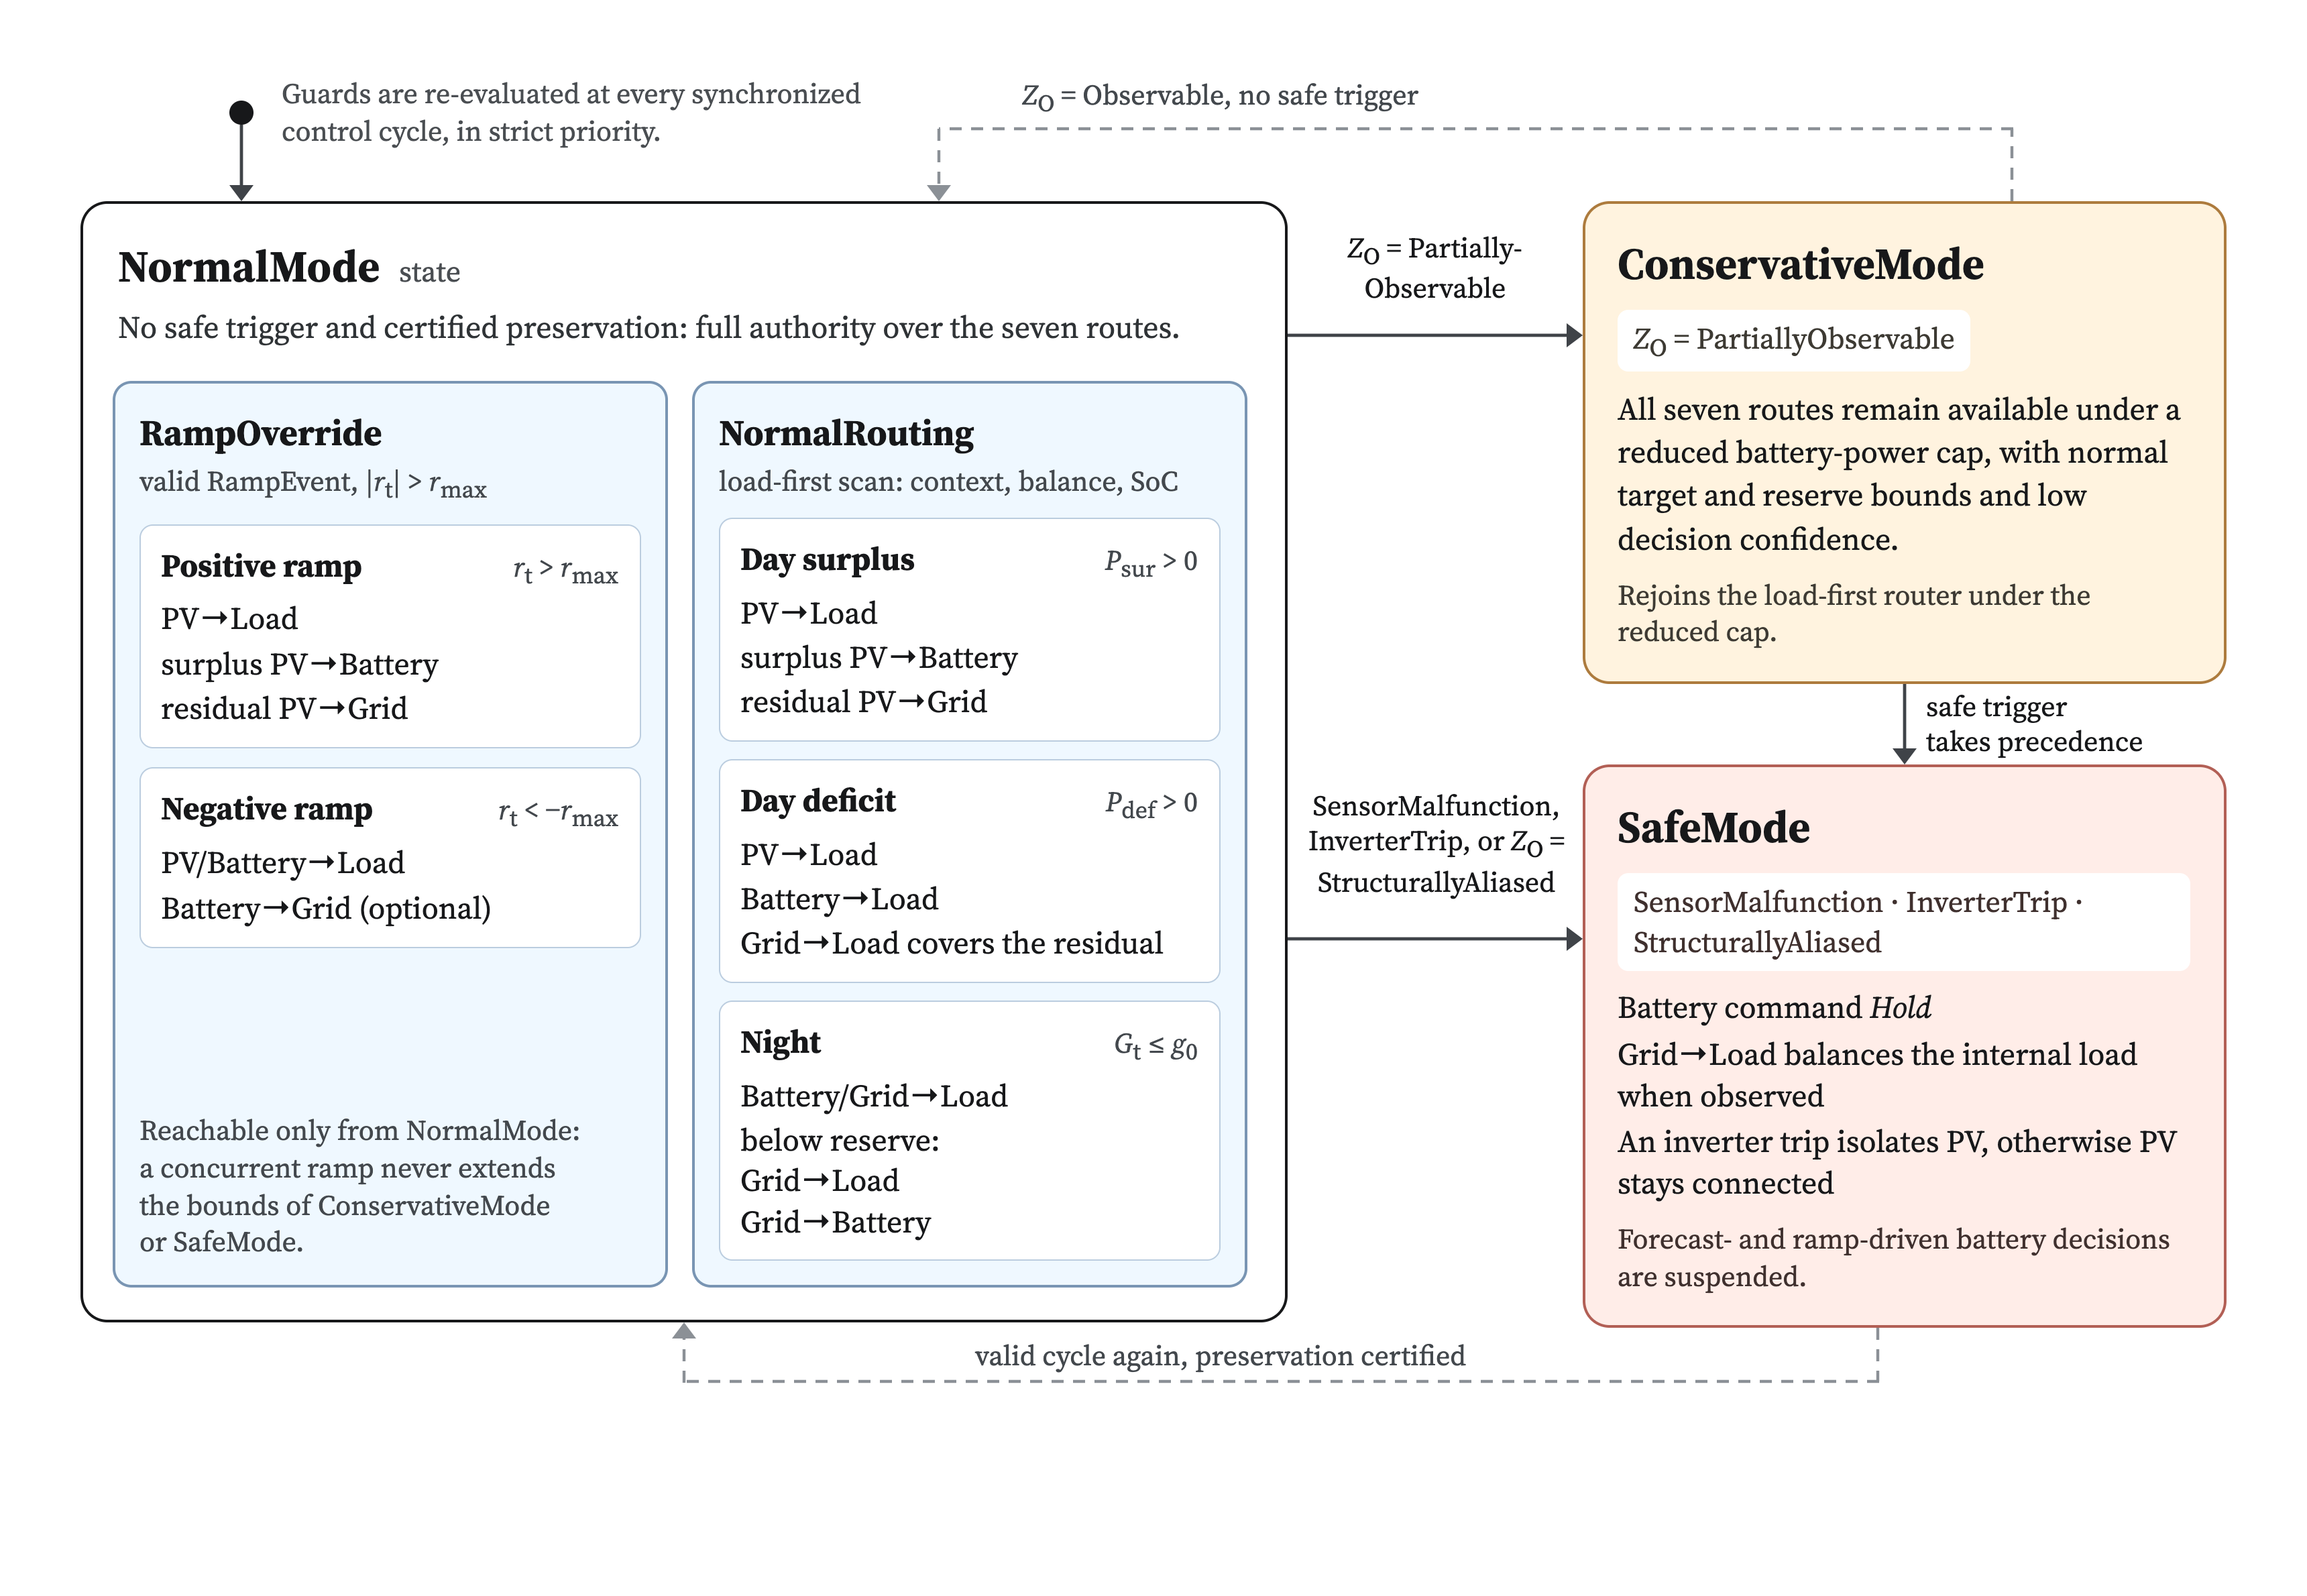
\includegraphics[width=\textwidth]{figures/routing.png}
\caption{The routing policy as a priority scan. The mode of \autoref{eq:mode-selection} is read first, so a safe-mode cycle never reaches the ordinary branches; the ramp branch is available only in \valueof{NormalMode}, and the conservative branch rejoins the ordinary load-first router under its reduced cap. Below that the surplus and deficit of \autoref{eq:surplus-deficit} decide which of the seven admissible routes of \autoref{eq:routes} a cycle issues, always serving the internal load before charging the battery or exporting. A cycle issues a route only for a strictly positive transfer and may issue several co-mode decisions, and every setpoint is clipped to the state of charge, the capacity and the charge and discharge limits; \autoref{tab:routing} states the boundary cases this diagram compresses.}
\label{fig:routing-policy}
\end{figure}

\begin{table}[!tbp]
\centering
\footnotesize
\begin{tabular}{@{}M{0.23\linewidth}M{0.29\linewidth}M{0.39\linewidth}@{}}
\toprule
\textbf{Condition} & \textbf{Ordered route set} & \textbf{Constraint} \\
\midrule
Daylight surplus & PV$\to$Load; PV$\to$Battery; PV$\to$Grid & Serve demand, charge to target, then export the residual. \\
\rowsep
Daylight deficit & PV$\to$Load; Battery$\to$Load; Grid$\to$Load & Discharge only to reserve; the grid covers the remaining deficit. \\
\rowsep
Night, $s>s_{\mathrm{reserve}}$ & Battery$\to$Load; Grid$\to$Load & Battery serves demand to reserve; the grid supplies the residual. \\
\rowsep
Night, $s\leq s_{\mathrm{reserve}}$ & Grid$\to$Load; if $s<s_{\mathrm{reserve}}$, Grid$\to$Battery & Supply the load first; charge only below reserve and stop at reserve. \\
\midrule
Positive ramp with surplus & PV$\to$Load; PV$\to$Battery; PV$\to$Grid & NormalMode may charge beyond target, never beyond maximum SoC. \\
\rowsep
Negative ramp with valid positive reference & load-serving routes; Battery$\to$Grid & Export only after serving the load, within residual discharge capacity and above reserve. \\
\rowsep
Negative ramp without usable reference & ordinary surplus/deficit routes & Missing, stale, non-finite, zero, or negative reference disables export catch-up. \\
\midrule
ConservativeMode & ordinary load-first routes & Reduced battery cap; target/reserve bounds; no ramp extensions. \\
\rowsep
SafeMode & Grid$\to$Load when observed & Battery Hold; grid Balance; isolate PV only for inverter trip. \\
\bottomrule
\end{tabular}
\caption{Routing matrix for the seven admissible transfer directions.}
\label{tab:routing}
\end{table}


For a negative ramp, Battery$\to$Grid is admissible only after the internal load has been fully served, the export reference is present, fresh, finite, and positive, measured export is below that reference, the battery remains above reserve, and discharge capacity remains after load support; if any condition fails, the ordinary load-first route applies. At night, Grid$\to$Battery begins only after Grid$\to$Load has been satisfied and stops when reserve is restored. These rules preserve \autoref{eq:power-balance} without turning the routing policy into a separate optimisation problem.

\endgroup

\flushfloatpages
\tablesbelowtext
\appendixsection{Chronos-Bolt-Tiny Retraining Procedure}{sec:appRetraining}
This appendix gives a high-level view of the training workflow, from selecting a patch geometry to saving its trained checkpoint.\footnote{The retraining procedure is implemented in \href{https://github.com/FedericoSabbadini/patchAliasing/blob/main/notebooks/chronos_architecture/train_sweep.py}{\texttt{train\_sweep.py}}.} The same controlled procedure is applied to each of the fifteen geometries of \autoref{tab:hfModels}: the required $(P,S)$ pairs are enumerated, crossed with the single training seed, and processed one after another, so that the geometry is the only thing that changes between runs\@. \autoref{tab:trainParams} collects every setting in one place, beside the published value it was taken from or departs from; the subsections below give the reasoning that the table cannot carry.

\begin{table}[!tbp]
    \centering
\footnotesize
    \setlength{\tabcolsep}{4pt}
    \begin{tabular}{@{}M{3.6cm}M{4.4cm}M{2.2cm}M{5.0cm}@{}}
        \toprule
        \multicolumn{4}{@{}l}{\textit{Tokenisation geometry (the swept parameters)}}\\
        \textbf{Parameter} & \textbf{Adopted} & \textbf{Published} & \textbf{Constraint / note} \\
        \midrule
        Patch size $P$              & $8$, $16$, $24$, $32$              & $16$                & swept; the pairs are in \autoref{tab:hfModels} \\
        \rowsep
        Stride $S$                  & $8$, $12$, $16$, $20$, $24$, $32$  & $16$                & swept, subject to $S\le P$ \\
        \rowsep
        Geometries trained          & $15$                               & $1$                 & one checkpoint per $(P,S)$ \\
        \rowsep
        Training seed               & $42$                               & ---                 & one seed, shared by every run \\
        \addlinespace[12pt]
        \midrule[\heavyrulewidth]
        \addlinespace[3pt]
        \multicolumn{4}{@{}l}{\textit{Architecture (fixed, from Chronos-Bolt-Tiny)}}\\
        \textbf{Parameter} & \textbf{Adopted} & \textbf{Published} & \textbf{Constraint / note} \\
        \midrule
        Context length              & $2048$ samples                     & $2048$              & as released \\
        \rowsep
        Prediction length           & $64$ samples                       & $64$                & as released \\
        \rowsep
        Quantile levels             & $9$, from $0.1$ to $0.9$           & $9$                 & as released \\
        \rowsep
        Widths, heads, layers       & as released                        & as released         & only $(P,S)$ is overridden \\
        \rowsep
        Initial weights             & random                             & pretrained          & every geometry trained from scratch \\
        \addlinespace[12pt]
        \midrule[\heavyrulewidth]
        \addlinespace[3pt]
        \multicolumn{4}{@{}l}{\textit{Data pipeline}}\\
        \textbf{Parameter} & \textbf{Adopted} & \textbf{Published} & \textbf{Constraint / note} \\
        \midrule
        Corpora (streamed)          & TSMixup $10$M, KernelSynth $1$M    & same                & public Chronos collection \\
        \rowsep
        Mixing ratio                & $9{:}1$                            & $9{:}1$             & TSMixup to KernelSynth \\
        \rowsep
        Shuffle buffer              & $10{,}000$                         & $100{,}000$         & departure: streaming throughput \\
        \rowsep
        Minimum observed past       & $60$ samples                       & $60$                & required before the horizon \\
        \rowsep
        Maximum missing per series  & $0.9$                              & $0.9$               & series above this are discarded \\
        \rowsep
        Injected missing rate       & $\mathcal U(0,0.2)$                & $\mathcal U(0,0.2)$ & masked, excluded from the loss \\
        \rowsep
        Windows per series          & $1$                                & $1$                 & one admissible split point \\
        \addlinespace[12pt]
        \midrule[\heavyrulewidth]
        \addlinespace[3pt]
        \multicolumn{4}{@{}l}{\textit{Optimisation}}\\
        \textbf{Parameter} & \textbf{Adopted} & \textbf{Published} & \textbf{Constraint / note} \\
        \midrule
        Gradient updates            & $100{,}000$                        & $200{,}000$         & departure: compute budget \\
        \rowsep
        Batch size                  & $32$ windows                       & $256$               & departure: one device, where the published $256$ is $8\times32$ \\
        \rowsep
        Windows seen                & $3.2$M                             & $51.2$M             & updates $\times$ batch size \\
        \rowsep
        Optimiser                   & AdamW                              & AdamW               & --- \\
        \rowsep
        Learning rate               & $10^{-3}$                          & $10^{-3}$           & --- \\
        \rowsep
        Scheduler / warmup          & linear to zero / none              & linear / none       & --- \\
        \rowsep
        Weight decay                & $0.0$                              & $0.01$              & as in the released script, which keeps the default $0.0$ \\
        \rowsep
        Gradient-norm clip          & $1.0$                              & $1.0$               & --- \\
        \rowsep
        Numerical precision         & single                             & TF32                & reduced-precision matrix products where available \\
        \bottomrule
    \end{tabular}
\caption{Training parameters of every retrained geometry, beside the published Chronos recipe\autocite{ansariChronosLearningLanguage2024} by which the not fully published Chronos-Bolt recipe is approximated, with the constraint behind each. The architecture rows follow the released Chronos-Bolt-Tiny configuration. Besides the patch geometry, the object of the study, the step budget, the batch and the shuffle buffer are reduced to fit the compute, identically for all fifteen runs, and the weight decay is that of the released script rather than of the article.}
    \label{tab:trainParams}
\end{table}


\subsection{Model construction}

The architectural configuration of Chronos-Bolt-Tiny \autocite{AmazonChronosbolttinyHugging2025,FastAccurateZeroshot2024a} is taken as published, but none of its pretrained weights are loaded. Encoder and decoder dimensions, attention heads and layer counts are preserved, the context and prediction lengths are fixed at $2048$ and $64$ samples, and the nine forecast quantiles from $0.1$ to $0.9$ are retained. Before the network is instantiated, the declared patch size and patch stride are replaced by $P$ and $S$; every weight is then initialised at random. The standard $P=S=16$ configuration is therefore retrained under the same budget as every variant rather than represented by the longer-trained published checkpoint, so that a comparison between geometries is not also a comparison between training histories.

\subsection{Streaming training data}

The training data follow the Chronos pretraining mixture\autocite{ansariChronosLearningLanguage2024,autogluonChronosDatasets2024}: the ten-million-series TSMixup corpus and the one-million-series KernelSynth corpus are read from the public Chronos dataset collection as streams rather than materialised, shuffled independently under the common seed, and interleaved in a $9{:}1$ ratio. The shuffle buffer holds ten thousand examples rather than the published hundred thousand, which trades a little mixing for a stream that does not stall.

Each training window is drawn under fixed admission rules: a series is used only if it offers at least $60+64$ samples, so that a $64$-sample horizon is always preceded by at least $60$ observed positions, and it is rejected outright if more than $90\%$ of its values are absent. A missingness rate is then drawn uniformly between $0$ and $0.2$ and that fraction of observations is marked as unobserved, after which one admissible split point is sampled: the most recent $2048$ values before it form the context, shorter histories being padded on the left, and the following $64$ form the target. Both arrays carry a mask of which positions are real, and a window whose context or target is entirely unobserved is discarded. Missingness is therefore preserved through the model's own normalisation step while unobserved target positions are excluded from the quantile loss, which is what keeps an artificial gap from being scored as a prediction error.

\subsection{Optimisation}

Each geometry is trained for one hundred thousand gradient updates on batches of thirty-two windows. The optimiser is AdamW with a learning rate of $10^{-3}$ decayed linearly to zero without warmup, and gradients are clipped at norm one, all as in the published recipe\autocite{ansariChronosLearningLanguage2024}. Computation is carried in single precision, with reduced-precision matrix products enabled where the device offers them, again as published. Four settings depart from that recipe (\autoref{tab:trainParams}). The published model takes $200{,}000$ updates on eight devices holding thirty-two windows each, so that a batch has $256$ windows and training covers $51.2$ million of them; the retrained models use one device and cover $3.2$ million, a sixteenth. The shuffle buffer is a tenth of the published size. The weight decay is $0.0$, the default that the released training script keeps, where the article reports $0.01$. The first three departures were forced by the compute and the streaming throughput available here\footnote{Retraining was performed on an Alienware 16 Aurora with a [CPU model to confirm], a single NVIDIA RTX 5060 Laptop GPU (8\,GB VRAM), and 32\,GB RAM.} rather than chosen, the last follows the released script, and all four apply identically to every geometry, the standard one included, so none can favour or penalise a particular $(P,S)$. The consequence to keep in mind is that all fifteen models are undertrained relative to the released checkpoint by the same amount, which makes them comparable with one another but not directly with the published model.

The fifteen checkpoints are published with a fixed revision\autocite{sabbadiniChronosBoltPatchSweep2026}. The reproduction therefore follows the released architecture and the published Chronos recipe in procedure, data mixture and optimiser family, but not in budget, batch size or weight decay. The training recipe of the released Chronos-Bolt checkpoint is not fully published, so that checkpoint may also differ in data and procedure, and every statement about geometry rests on comparisons among the retrained models alone. The published $P=S=16$ checkpoint is nonetheless kept beside them as a reference baseline, despite its different budget, because it measures how far the reduced budget leaves the retrained models from the original. On the photovoltaic series, for instance, the retrained $P=S=16$ trails it by about $2.5$\,W of mean absolute error (\autoref{tab:solarVsOfficial}), and on generated signals it returns added components less often (\autoref{tab:decomposition}). Differences of that size between the published and a retrained model are read as the cost of the budget and of any difference in recipe, not as an effect of the geometry.


\flushfloatpages
\appendixsection{Light TSMixup}{sec:appTSMixup}
\begin{algorithm}[H]
\caption{Light TSMixup: background generation from a sinusoidal frequency pool}%
\label{alg:light_tsmixup}
\begin{algorithmic}[1]
\Require Frequency pool $\mathcal{P}=\{f_1,\ldots,f_M\}$ in Hz, with $M=574$ spanning $2$ to $250$\,Hz, built from the design as described in this appendix; maximum components $K=10$; symmetric Dirichlet concentration $\alpha=1.5$; draw length $l$, the probing context plus the forecast horizon; sampling frequency $f_s$.
\Ensure One background realisation $x_{1:l}$ of unit variance.
\For{$m \gets 1$ to $M$}
    \State $x^{(m)}_{1:l} \gets \sin\!\left(2\pi f_m\, n / f_s\right),\ n=0,\ldots,l-1$ \Comment{one sinusoid per pool frequency}
\EndFor%
\State $k \sim U\{1,K\}$ \Comment{number of components to mix}
\For{$i \gets 1$ to $k$}
    \State $m \sim U\{1,M\}$ \Comment{draw a source, with replacement}
    \State $\tilde{x}^{(i)}_{1:l} \gets x^{(m)}_{1:l} \Big/ \left(\frac{1}{l}\sum_{j=1}^{l}\left|x^{(m)}_j\right|\right)$ \Comment{apply mean scaling}
\EndFor%
\State $[\lambda_1,\ldots,\lambda_k] \sim \operatorname{Dir}([\alpha_1=\alpha,\ldots,\alpha_k=\alpha])$ \Comment{sample mixing weights}
\State $x_{1:l} \gets \sum_{i=1}^{k}\lambda_i\tilde{x}^{(i)}_{1:l}$ \Comment{take a weighted combination of scaled sources}
\State \Return $x_{1:l} / \operatorname{std}\!\left(x_{1:l}\right)$ \Comment{unit variance, so the injected tone sets a true SNR}
\end{algorithmic}
\end{algorithm}


\medskip 

Light TSMixup is a variant of the TSMixup augmentation described in the Chronos data-generation procedure\autocite{ansariChronosLearningLanguage2024}. The original algorithm samples subsequences from a collection of real training datasets, applies mean scaling to each sampled series, draws mixing coefficients from a symmetric Dirichlet distribution and returns their convex combination. The variant used here preserves that stochastic mixing structure and replaces the real dataset collection with a pool of sinusoidal sources of known frequency, so that every generated series remains a superposition of known components and no loss measured at a predicted site can be attributed to unknown spectral content in the background.

\subsection{The source pool}

The pool holds $574$ unit-amplitude sinusoids, one per frequency, and is built from the design rather than fixed by hand: adding a geometry to \autoref{tab:hfModels} adds its own frequencies automatically. It spans the analysed band, $2$ to $250$\,Hz, so no part of that band is silent in the background, and it has four parts.

The first is every integer frequency from $2$ to $250$\,Hz, which is $249$ sources. Covering the integer grid uniformly is what keeps the pool neutral with respect to the hypotheses: a candidate frequency is represented in the background exactly as the frequencies flanking it are, so the background cannot by itself make a candidate easier or harder to recover than its controls.

The second is the sixteen members of $\mathcal F_{\mathrm{lock}}$ inside the band that are not integers, which the first part cannot reach. They arise in the geometries whose stride or patch size is $12$, $20$ or $24$, where $f_s/S$ or $f_s/P$ is not a whole number of hertz: the stride comb of $S=12$ falls, among others, at $42.\overline{6}$ and $85.\overline{3}$\,Hz, and those of $S=20$ and $S=24$ at multiples of $25.6$ and $21.\overline{3}$\,Hz. Without them the pool would represent the integer candidates and omit the rest.

The third is the control frequencies $f_k\pm\delta$ of every candidate that falls in the pool's range, $248$ distinct values of which $159$ are not already integers. They matter for the same reason the integer grid does, and more sharply. The offset $\delta$ is chosen per site as the largest one, up to a quarter of the stride spacing, that keeps both controls at least one hertz from every other candidate (\autoref{sec:appBayes}), so it is rarely a whole number of hertz: without this group every locked arm of a contrast triplet would sit on a pool frequency while fewer than half the control arms would, and the background would carry a little more energy on one side of \autoref{eq:d2contrast} than on the other. Since that contrast assumes its three arms differ only in frequency, the asymmetry would be indistinguishable from the effect $H1$ is meant to detect. With the controls in the pool both arms are covered alike.

The fourth is $150$ further non-integer frequencies spread evenly across the band, each held at least $0.2$\,Hz away from every candidate and from the integer grid. They give the background content that no geometry predicts, which is what prevents the pool from being a description of $\mathcal F_{\mathrm{lock}}$ and its controls and nothing else.

\subsection{Generation}

One realisation is produced by drawing a number of components $k$ uniformly between one and the maximum $K$, drawing that many sources from the pool with replacement, scaling each by the reciprocal of its mean absolute value, and returning their convex combination under weights drawn from a symmetric Dirichlet distribution of concentration $\alpha$. The values adopted are $K=10$ and $\alpha=1.5$, and every source is generated at the full draw length, the probing context plus the forecast horizon, so no source is tiled or truncated. Drawing with replacement means a frequency may enter one mixture more than once, and a mixture therefore carries at most ten of the $574$ frequencies: a single background is sparse in that range even though the pool is dense in it.

Two properties of the generator matter. The concentration $\alpha$ sets how evenly the mixing weights are spread, so values near zero return something close to a single sinusoid while larger values return balanced mixtures; at $\alpha=1.5$ the components are comparable in size without being equal. Because the sources are defined in hertz rather than in cycles per sample, the pool is tied to the sampling rate, hence to the lock arithmetic of \autoref{eq:flock}: the same construction at a different $f_s$ yields a different pool, which is the intended behaviour.

The probe tone is not part of this generator: a realisation is normalised to unit variance and the tone is added afterwards, at the frequency and phase the design requires and at amplitude $1.5$, which fixes its signal-to-noise ratio against the normalised background, so the background and the quantity under test are produced independently of one another.

\autoref{alg:light_tsmixup} states the procedure step by step, with the values adopted here; the pool it takes as input is the one described in this appendix.

\flushfloatpages
\appendixsection{KernelSynth}{sec:appKernelSynth}
\begin{algorithm}[H]
\caption{KernelSynth: Synthetic Data Generation using Gaussian Processes}
\label{alg:kernelsynth}
\begin{algorithmic}[1]
\Require Kernel bank $\mathcal{K}$ listed in \autoref{tab:kernelsynth_bank}; maximum kernels per time series $J=5$; generated length $l_{\mathrm{syn}}=544$; numerical jitter $\epsilon=10^{-4}$.
\Ensure A synthetic time series $x_{1:l_{\mathrm{syn}}}$.
\State $j \sim U\{1,J\}$ \Comment{sample the number of kernels}
\State $\{\kappa_1(t,t'),\ldots,\kappa_j(t,t')\} \overset{\mathrm{i.i.d.}}{\sim} \mathcal{K}$ \Comment{sample kernels with replacement}
\State $t \gets \operatorname{linspace}(0,1,l_{\mathrm{syn}})$
\State $\kappa^\star(t,t') \gets \kappa_1(t,t')$ \Comment{initialise the composite covariance}
\For{$i \gets 2$ to $j$}
    \State $\star \sim U\{+,\times\}$ \Comment{sample a binary composition operator}
    \State $\kappa^\star(t,t') \gets \kappa^\star(t,t') \star \kappa_i(t,t')$ \Comment{compose kernels}
\EndFor
\If{$\epsilon > 0$}
    \State $\kappa^\star(t,t') \gets \kappa^\star(t,t') + \epsilon I$
\EndIf
\State $x_{1:l_{\mathrm{syn}}} \sim \mathcal{GP}(0,\kappa^\star(t,t'))$ \Comment{sample from the GP prior}
\State \Return $x_{1:l_{\mathrm{syn}}}$
\end{algorithmic}
\end{algorithm}

\medskip

KernelSynth is the Gaussian-process generator of the Chronos data-generation procedure\autocite{ansariChronosLearningLanguage2024}. Where Light TSMixup can only produce superpositions of sinusoids, KernelSynth composes covariance functions and samples from the resulting prior, so its output carries trends, non-stationary structure and broadband content as well as periodicity. It is included precisely because a phenomenon that appears only on tones and simple mixtures would be an artefact of the probe; a phenomenon that survives on signals resembling the corpus the model was trained on is a property of the model.

The procedure draws $j$ kernels with replacement from a fixed bank $\mathcal K$, composes them pairwise under a binary operator sampled between sum and product, and draws one realisation from the zero-mean Gaussian process with the composite covariance. Sum composition superposes two behaviours, so a periodic kernel added to a linear one produces an oscillation riding on a trend; product composition modulates one by the other, so the same pair multiplied produces an oscillation whose amplitude grows along the series. Sum and product compositions of the same kernels therefore yield very different series.

\newpage
% The bank table follows all the text of Appendix D and is set at the top or bottom of a page.
\begin{table}[!t]
\small
\centering
\renewcommand{\arraystretch}{1.25}
\begin{tabular}{M{0.21\linewidth} M{0.38\linewidth} M{0.32\linewidth}}
\toprule
Kernel & Formula & Hyperparameters \\
\midrule
Constant &
$\kappa_{\mathrm{Const}}(x,x')=C$ &
$C=1$ \\
\rowsep%
White Noise &
$\kappa_{\mathrm{White}}(x,x')=\sigma_n \cdot \mathbf{1}_{x=x'}$ &
$\sigma_n \in \{0.1,1\}$ \\
\rowsep%
Linear &
$\kappa_{\mathrm{Lin}}(x,x')=\sigma_0^2+x\cdot x'$ &
$\sigma_0 \in \{0,1,10\}$ \\
\rowsep%
RBF &
$\kappa_{\mathrm{RBF}}(x,x')=\exp\!\left(-\frac{\lVert x-x'\rVert^2}{2l^2}\right)$ &
$l \in \{0.1,1,10\}$ \\
\rowsep%
Rational Quadratic &
        $\kappa_{\mathrm{RQ}}(x,x')=\left\lparen1+\frac{\lVert x-x'\rVert^2}{2\alpha}\right\rparen^{-\alpha}$ &
$\alpha \in \{0.1,1,10\}$, $l=1$ \\
\rowsep%
Periodic &
$\kappa_{\mathrm{Per}}(x,x')=\exp\!\left(-2\sin^2\!\left(\pi\frac{\lVert x-x'\rVert}{p/l_{\mathrm{syn}}}\right)\right)$ &
\begin{tabular}[t]{@{}l@{}}
$p \in \{24,48,96,168,336,672\mathpunct{,}$\\
$7,14,30,60,365,730\mathpunct{,}$\\
$4,26,52,4,6,12,4,40,10\}$
\end{tabular} \\
\bottomrule
\end{tabular}
\caption{Kernel bank $\mathcal{K}$ used by KernelSynth.}%
\label{tab:kernelsynth_bank}
\end{table}


Three parameters control the output. The maximum number of kernels $J$ bounds the compositional depth, and therefore how far a draw can depart from the behaviour of a single kernel. The generated length $l_{\mathrm{syn}}$ fixes the support of the covariance, and enters the periodic kernel through the ratio $p/l_{\mathrm{syn}}$ on a time axis rescaled to $[0,1]$, so each period value of \autoref{tab:kernelsynth_bank} is a number of samples whatever the length of the series; repeated values are kept as in the original bank, which weights the draw towards them. The jitter $\epsilon$ is a numerical term added to the diagonal to keep the covariance positive definite. In this study every draw is generated directly at the length it is used for, $l_{\mathrm{syn}}=480+64=544$ samples, with $\epsilon=10^{-4}$, rather than cut from a longer series; it is then standardised to zero mean and unit variance, the first $480$ samples form the context and the last $64$ the real continuation. \autoref{alg:kernelsynth} states the procedure and \autoref{tab:kernelsynth_bank} the bank, with the hyperparameter values each kernel is drawn from: the length scale $l$ of the radial basis function (RBF) kernel and the shape $\alpha$ of the rational quadratic control how quickly the process decorrelates, the noise scale $\sigma_n$ how much unstructured content is added, and the period set of the periodic kernel spans the daily, weekly, monthly and yearly cycles of the original recipe.




\flushfloatpages
\tablesbelowtext
\appendixsection{Bayesian Model Specifications}{sec:appBayes}
This appendix states in full the five models summarised in \autoref{sec:models} and the reading of Model~A that carries the mitigation claim $M1$, as they are implemented in the analysis notebook released with this report.\footnote{The analysis is implemented in the notebook \href{https://github.com/FedericoSabbadini/patchAliasing/blob/main/notebooks/bayesian/deliverable3_bayesian_models.ipynb}{\texttt{deliverable3\_bayesian\_models.ipynb}}.} For each model it gives what is measured and how, the likelihood and the linear predictor, the meaning, index and prior of every term, the estimand and the rule that decides it. The validation every fit must pass before it is read is stated at the end, together with the limitations of the design.

\subsection{Model A, the behavioural reading (H1)}

\paragraph{Measurement.} For every geometry, each candidate frequency $f_k\in\mathcal F_{\mathrm{lock}}$ is paired with two controls $f_k\pm\delta$, where $\delta$ is the largest offset not exceeding $0.25\,f_s/S$ that keeps both controls at least $1$\,Hz from every other candidate; a site with no such offset is dropped. The candidate is injected at its exact value, the non-integer sites included. Each of the three arms is a tone of amplitude $1.5$ added to a unit-variance background, with $100$ Light TSMixup and $100$ KernelSynth backgrounds and up to ten non-redundant starting phases per candidate. The three arms of a triplet share their background realisation and their phase, so only the frequency changes. The model receives the first $480$ samples and forecasts the next $64$, and the amplitude recovery of an arm is
\begin{equation*}
R=\frac{A_{\mathrm{pred}}}{A_{\mathrm{true}}},
\end{equation*}
the least-squares amplitude of the median forecast at the arm's own frequency over that of the true continuation there. The injected amplitude is recorded as well, and the same contrast formed with it is reported beside the fitted one as a check on the choice of denominator. The triplet is reduced to one contrast,
\begin{equation}
\label{eq:appA:contrast}
d = \log(R_k + 0.01) - \tfrac{1}{2}\left[\log(R_- + 0.01) + \log(R_+ + 0.01)\right],
\end{equation}
negative when the candidate recovers less than its neighbours. The stabiliser $0.01$ keeps the logarithm finite where a forecast rebuilds nothing, and every complete triplet is fitted: no response filter is applied after collection.

\paragraph{Model.}
\begin{equation}
\label{eq:appA:model}
d_i \sim \text{Student-}t_4(\mu_i,\ \sigma),
\quad
\mu_i = \beta_{c[i]} + u_{k[i]} + u_{b[i]},
\quad
\beta_c \sim \mathcal{N}\!\left(\bar\beta + \delta_O \widetilde O_c + \delta_P \widetilde{\log P}_c,\ \tau\right).
\end{equation}
\autoref{tab:termsA} gives every term with its meaning and number of levels. It separates the two estimands the claims read, $\bar\beta$ for $H1$ and $\delta_O$ for $M1$, from the patch-size slope $\delta_P$ that keeps patch size apart from overlap, and from the offsets and scales that absorb what a triplet does not cancel: the candidate frequency, the background realisation and the residual. The response is a paired difference rather than a level, so no lock indicator is needed and the effect of interest is the population intercept $\bar\beta$. The Student-$t_4$ likelihood admits the very negative contrasts of the arms that rebuild nothing without letting a handful of them set the estimate, which a Gaussian would. The configuration effects are drawn around a population mean, which makes the fifteen geometries instances of one phenomenon and gives each of them equal weight, however many triplets it contributes.

\begin{table}[!tbp]
    \centering
    \small
    \setlength{\tabcolsep}{4pt}
    \renewcommand{\arraystretch}{1.2}
    \begin{tabular}{@{}lM{9.6cm}l@{}}
        \toprule
        \textbf{Term} & \textbf{Meaning} & \textbf{Levels} \\
        \midrule
        $d_i$ & contrast of triplet $i$, \autoref{eq:appA:contrast} & one per triplet \\
        \rowsep
        $\beta_c$ & mean contrast of geometry $c$ & $15$ \\
        \rowsep
        $\bar\beta$ & \textbf{estimand of $H1$}: population contrast at the average configuration; $e^{\bar\beta}$ is recovery at a candidate relative to its controls & $1$ \\
        \rowsep
        $\delta_O$ & \textbf{estimand of $M1$}: change of $\beta_c$ per unit of centred overlap & $1$ \\
        \rowsep
        $\delta_P$ & change of $\beta_c$ per unit of centred $\log P$; keeps patch size from loading onto $\delta_O$ & $1$ \\
        \rowsep
        $\widetilde O_c$, $\widetilde{\log P}_c$ & $(O_c-\bar O)/0.5$ and $\log P_c-\overline{\log P}$, averages over the fifteen geometries & data \\
        \rowsep
        $\tau$ & spread of the geometries around the regression, what the two covariates leave unexplained & $1$ \\
        \midrule
        $u_k$ & offset of candidate frequency $k$, a value shared by every geometry in which it is a candidate; sum to zero & one per frequency \\
        \rowsep
        $u_b$ & offset of background realisation $b$, indexed by generator and draw; sum to zero & $200$ \\
        \rowsep
        $\sigma_k$, $\sigma_b$ & scales of $u_k$ and $u_b$ & $1$ each \\
        \rowsep
        $\sigma$ & residual scale of the Student-$t_4$ likelihood & $1$ \\
        \bottomrule
    \end{tabular}
    \caption{Terms of Model~A.}
    \label{tab:termsA}
\end{table}


\paragraph{Estimand and rule.} $H1$ predicts $e^{\bar\beta}<1$; it is supported when $\Pr(\bar\beta<\log 0.8\mid D)\ge0.95$, a recovery at a candidate of at most four fifths of its controls, and refuted when $\Pr(|\bar\beta|<\log1.1\mid D)\ge0.95$. Centring the covariates is what makes $\bar\beta$ the effect at the average geometry of the design rather than an extrapolation to $O=0$ and a patch of one sample.

\subsection{\texorpdfstring{Model A$'$}{Model A'}, the mitigation claim (M1)}

$M1$ claims that the loss Model~A measures is smaller where consecutive patches overlap more. It is not a separate fit but the configuration level of \autoref{eq:appA:model} read as an estimand, drawn from the same chains and the same rows as $\bar\beta$:
\begin{equation}
\label{eq:appM1:model}
\beta_c \sim \mathcal{N}\!\left(\bar\beta + \delta_O \widetilde O_c + \delta_P \widetilde{\log P}_c,\ \tau\right),
\qquad
\widetilde O_c=\frac{O_c-\bar O}{0.5},
\qquad
\widetilde{\log P}_c=\log P_c-\overline{\log P},
\end{equation}
with $O_c$ the overlap ratio of \autoref{eq:overlap}. One unit of $\widetilde O$ corresponds to $0.5$ of $O$, so the design spans from $\widetilde O=-0.66$ at $O=0$ to $0.84$ at $O=0.75$. The response rises towards zero as recovery at a candidate approaches recovery at its controls, so an overlap that mitigates raises $\beta_c$ and $M1$ predicts $\delta_O>0$.\footnote{Deliverable~2 printed this rule with the opposite sign, $\delta_O<0$, an inconsistency the review of Deliverable~2 pointed out. With the contrast defined as the candidate minus its controls, a mitigation raises it, so only the positive sign reads as a mitigation. Deliverable~2 also read a supported $M1$ as overlap reducing the deficit; it is read here as an association across geometries, because each geometry is a separately trained model from a single seed, so the slope compares different models rather than measuring what a change of overlap does to one of them.} This reading of the sign presumes a loss at the candidates, $\bar\beta<0$; where candidates recover more than their controls, a positive $\delta_O$ would instead mean that overlap enlarges the gain, so $M1$ is read conditionally on the direction of $\bar\beta$, as $H2$ is on the size of its effect. Patch size enters as $\log P$ because the patch comb has spacing $f_s/P$, so equal steps in $\log P$ are equal ratios of spacing. The two covariates are estimable together because \autoref{tab:hfModels} varies $S$ at fixed $P$ and $P$ at fixed $S$: their correlation across the fifteen runs is $0.43$, far from the degeneracy of a design in which overlap could be raised only by enlarging the patch.

The rule has two legs, both required: $\Pr(\delta_O>0\mid D)\ge0.95$, and the model with the overlap term must win the leave-one-out comparison against the same model without it. $M1$ is refuted when $\Pr(\delta_O>0\mid D)$ falls to $0.05$ or when the equivalence rule $\Pr(|\delta_O|<\log1.1\mid D)\ge0.95$ holds, half a unit of overlap moving the loss by under ten per cent. The equivalence rule takes the form of the one for $H1$, so that an effect credibly too small to matter refutes $M1$ as it refutes $H1$. The second leg is needed because a sign probability starts at $0.50$ under a prior symmetric about zero, so a small but consistently signed slope would otherwise count as a mitigation. The slope compares independently trained variants over fifteen design points, so a supported $M1$ is evidence that the effect varies with geometry in the predicted direction across this grid, not the effect of changing the overlap of one trained model.

\subsection{Model B, the representational reading (H1)}

\paragraph{Measurement.} A cell is one geometry, one probe stage and one centre frequency $f_c$. The centres are exactly the frequencies the triplets visit, every candidate and its two controls, so locked and non-locked centres stand in the ratio $1{:}2$ by construction. In each cell a linear probe must tell a tone at $f_c-1$\,Hz from one at $f_c+1$\,Hz, both added at amplitude $1.5$ to backgrounds of the two generators, with forty examples per class spread over ten background draws and ten phases per generator. The state is read at ten stages: the encoder $[\mathrm{REG}]$ token after each of the four encoder blocks, the decoder state after each of the four decoder blocks, the pre-projection vector and the output quantile head. The decoder vectors are called decoder states because Chronos-Bolt-Tiny carries $[\mathrm{REG}]$ in the encoder only and enters the decoder through a single start token. The probe is scored by its prequential description length\autocite{voitaInformationTheoreticProbingMinimum2020}: the examples are shuffled and split into five chunks, the first is charged one bit per label, and each later chunk is encoded by a probe trained only on the chunks before it, so a probe that memorises noise pays for itself. Inside each training chunk the state is standardised and reduced to its leading twenty principal components before a logistic regression is fitted, so the codelength prices only what is linearly decodable from that subspace; low-variance directions that still carry frequency information may be discarded, and the measurement is a lower bound on what the state holds.

\paragraph{Model.}
\begin{equation*}
L_i \sim \text{Gamma}\!\left(r,\ r/\mu_i\right),
\qquad
\log \mu_i = \alpha_0 + \theta_{\mathrm{lock}}\,\mathrm{IsLocked}_i + s_{\text{st}[i]} + g_{\text{geo}[i]}.
\end{equation*}
A codelength is strictly positive, right-skewed and has a variance that grows with its mean, which is what a Gamma likelihood in its shape--rate form with a log link is for; its mean is $\mu_i$ and its coefficient of variation $1/\sqrt r$. \autoref{tab:termsB} gives the terms and their levels. The estimand is $\theta_{\mathrm{lock}}$, read on the lock indicator; the baseline $\alpha_0$, the stage offsets $s_{\text{st}}$ and the geometry offsets $g_{\text{geo}}$ absorb level differences unrelated to locking, and the shape $r$ carries the dispersion of the codelength.

\begin{table}[!tbp]
    \centering
    \small
    \setlength{\tabcolsep}{4pt}
    \renewcommand{\arraystretch}{1.2}
    \begin{tabular}{@{}lM{9.6cm}l@{}}
        \toprule
        \textbf{Term} & \textbf{Meaning} & \textbf{Levels} \\
        \midrule
        $L_i$ & prequential codelength of cell $i$, in bits & one per cell \\
        \rowsep
        $\mathrm{IsLocked}_i$ & $1$ when the centre $f_c$ is a candidate of that geometry, $0$ when it is a control & data \\
        \rowsep
        $\theta_{\mathrm{lock}}$ & \textbf{estimand}: log expansion of the codelength at a candidate; $e^{\theta_{\mathrm{lock}}}$ is the factor by which the labels cost more & $1$ \\
        \midrule
        $\alpha_0$ & baseline log codelength; prior centred on the log of the mean observed codelength & $1$ \\
        \rowsep
        $s_{\text{st}}$ & offset of the probe stage; sum to zero, scale $\sigma_{st}$ & $10$ \\
        \rowsep
        $g_{\text{geo}}$ & offset of the geometry; sum to zero, scale $\sigma_{geo}$ & $15$ \\
        \rowsep
        $r$ & Gamma shape, which carries the dispersion & $1$ \\
        \bottomrule
    \end{tabular}
    \caption{Terms of Model~B.}
    \label{tab:termsB}
\end{table}


\paragraph{Estimand and rule.} $H1$ predicts $e^{\theta_{\mathrm{lock}}}>1$, more bits to read a candidate frequency. It is supported when $\Pr(\theta_{\mathrm{lock}}>\log1.2\mid D)\ge0.95$, at least twenty per cent more code, and refuted when $\Pr(|\theta_{\mathrm{lock}}|<\log1.1\mid D)\ge0.95$. The stage and geometry offsets absorb level differences that run to several-fold and would otherwise be available to the lock indicator; the unadjusted form without them is fitted alongside and compared by leave-one-out, and the comparison is reported beside the verdict without deciding it. The seven hierarchical band tasks of \autoref{sec:appSweep} each summarise hundreds of frequencies in one codelength, so the lock indicator has nothing to attach to there; they remain a descriptive cross-check and are not fitted.

\subsection{Model C, the phase reading (H2)}

\paragraph{Model.} Model~C uses the triplets of Model~A with the phase kept rather than pooled. Its response is the per-phase deficit $y_i=-d_i$, positive when the candidate is worse, and the phase angle, taken modulo $2\pi$, is cut into eight equal slices, each with its own offset:
\begin{equation*}
y_i \sim \text{Student-}t_4(\mu_i,\ \sigma),
\qquad
\mu_i = \beta_{c[i]} + u_{k[i]} + u_{b[i]} + u_{p[i]},
\qquad
u_p = \sigma_\phi z_p .
\end{equation*}
The terms $\beta_c$, $u_k$, $u_b$, $\sigma$ and the scales are those of \autoref{tab:termsA}, read on the deficit and therefore with the opposite sign; $\beta_c$ is drawn around $\bar\beta$ alone, because $H2$ is not a question about the design axes and the covariates are dropped. The slice offsets $u_p$, eight levels, are written in non-centred form, with $z_p$ standard normal and constrained to sum to zero, and $\sigma_\phi$ is their scale. Slices are preferred to a fitted sinusoid because they presuppose no shape: any systematic dependence on the starting phase widens the spread.

\paragraph{Estimand and rule.} The estimand is $\sigma_\phi$, and $H2$ is supported when $\Pr(\sigma_\phi<\log1.1\mid D)\ge0.95$, a phase that moves the deficit by under ten per cent, and refuted when that probability falls to $0.05$. Under the sum-to-zero constraint each offset has standard deviation $\sigma_\phi\sqrt{7/8}$, so $\sigma_\phi$ is the scale parameter and not the realised spread of the eight offsets; the rule is applied to the parameter and the realised spread is reported beside it. The leave-one-out comparison against the same model without $u_p$ is the evidential reading and is reported without deciding the verdict. Where the population deficit is itself indistinguishable from zero little remains for phase to move, so $H2$ is read conditionally on it.

\subsection{Model D1, the location of the sites (H3)}

\paragraph{Measurement.} The token collapse $z_g(f)$ is the standard deviation of the input-patch embeddings across the patches of one context, averaged over the $256$ embedding dimensions. It is read at the output of the learned patch-embedding layer, before any transformer block: it is exactly zero whenever consecutive patches are identical, whatever the weights, which is the degeneracy the stride condition predicts, while the depth of a dip that is not exact, on the patch branch among others, also depends on that learned layer. It is swept on a one-hertz grid in union with the exact predicted sites of all fifteen geometries, the non-integer ones such as $42.\overline{6}$\,Hz for $S=12$ and $21.\overline{3}$\,Hz for $S=24$ included, in three signal modes: a pure sinusoid, and a tone of amplitude $1.5$ on a Light TSMixup or a KernelSynth background, three replicates each. Every curve is divided by its own off-grid median, so dip depths are comparable across geometries and replicates.

\paragraph{Model.}
\begin{equation*}
\log z_g(f) \sim \mathcal{N}\!\left(
\alpha_g + \theta_S \cdot \text{OnStrideGrid} + \theta_P \cdot \text{OnPatchGrid},\ \sigma
\right),
\end{equation*}
with the terms of \autoref{tab:termsD}, which lists Models~D1 and~D2. For Model~D1 the estimands are the dip depths $\theta_S$ and $\theta_P$ on the two grids, each measured against the off-grid level $\alpha_g$ of its geometry. A frequency is on a grid when it coincides with a member of that comb to within $10^{-6}$\,Hz, which the union grid makes possible; a one-hertz tolerance would also label the integer neighbours of a non-integer site, which lie on no comb, and it is fitted only as a robustness reading. The logarithm makes the labels multiplicative on the per-geometry off-grid level. On a pure sinusoid the collapse is exactly zero at a stride site, so that mode is floored at $0.01$ of the off-grid median before the logarithm. It is fitted and reported, but the verdict is read from the two generator modes: on the pure mode the response at a site depends on the floor, and a stratum of identical values has no dispersion for a predictive check to reproduce.

\paragraph{Estimand and rule.} Four labellings are fitted to the same profiles, both grids, stride only, patch only and neither, separately for each generator. $H3$ is supported when the two-label fit wins the leave-one-out comparison against the others and the joint posterior probability $\Pr(\theta_S<0\wedge\theta_P<0\mid D)$ reaches $0.95$, on both generators; the verdict takes the less favourable of the two. The joint event is used because the hypothesis is a conjunction, and two marginals above $0.95$ can accompany a joint probability below it.\footnote{Deliverable~2 asked of $H3$ only two negative coefficients and a winning fit. The joint reading replaces that rule, and it is required on both generator modes so that no single background carries the verdict.} $H3$ is refuted when the joint probability falls to $0.05$, or by an equivalence rule in the form of the one for $H1$: on both generators, $\Pr(|\theta_S|<\log1.1\lor|\theta_P|<\log1.1\mid D)\ge0.95$, one of the two grids carrying a practically nil dip, which denies the conjunction. The two coefficients separate only where one label applies without the other, which for $\theta_S$ means the six geometries with $S\nmid P$: where $S$ divides $P$, in nine runs including the four with $P=S$, every stride site is also a patch site.

\subsection{Model D2, the movement of the sites (H3a, H3b)}

\paragraph{Measurement.} Sites are detected on each collapse profile of the two generator modes as local minima reaching at most three quarters of the median of the profile within $\pm6$\,Hz, and detections closer than $1.5$\,Hz are merged. Each site is assigned to the branch whose comb lies within $1.5$\,Hz of it; a site compatible with both branches to within $0.25$\,Hz is set aside, because $\mathcal F_{\mathrm{lock}}$ is a union and the union of two combs has two interlaced spacings rather than one. The fundamental $\hat f^{\,F}_{1,g}$ of branch $F$ is its lowest assigned site on one replicate.

\paragraph{Model.}
\begin{equation*}
\hat f^{\,F}_{1,g} \sim \mathcal{N}\!\left(
\kappa_F \,\Delta^F_g,\ \sqrt{\sigma_F^2+\Delta f^2}
\right),
\qquad
\Delta^S_g=\frac{f_s}{S_g}, \quad \Delta^P_g=\frac{f_s}{P_g},
\end{equation*}
with the terms of \autoref{tab:termsD}, where the lower block holds the terms of this model: the measured fundamental, the spacing its branch predicts, the estimand $\kappa_F$ and the scatter $\sigma_F$ beyond the resolution floor $\Delta f$. The slope $\kappa_F$ is measured spacing per unit of predicted spacing, and its prior is centred on zero, that is on no relationship, so the hypothesis has to be earned from the data. The floor $\Delta f=1$\,Hz, the sweep step, is part of the residual because a spacing read off a discrete grid is no more precise than one step; without it, sites landing exactly on the prediction drive $\sigma_F$ to zero and the posterior develops a funnel the sampler cannot traverse. The median gap between successive sites is fitted in the same form as a robustness reading.

\begin{table}[!tbp]
    \centering
    \small
    \setlength{\tabcolsep}{4pt}
    \renewcommand{\arraystretch}{1.2}
    \begin{tabular}{@{}lM{9.6cm}l@{}}
        \toprule
        \textbf{Term} & \textbf{Meaning} & \textbf{Levels} \\
        \midrule
        \multicolumn{3}{@{}l}{\textit{Model D1, one fit per signal mode and labelling}}\\
        $\log z_g(f)$ & log token collapse of geometry $g$ at swept frequency $f$, one replicate & one per row \\
        \rowsep
        $\alpha_g$ & off-grid level of geometry $g$ & $15$ \\
        \rowsep
        $\theta_S$, $\theta_P$ & \textbf{estimands}: log depth of the dip on the stride and on the patch grid & $1$ each \\
        \rowsep
        OnStrideGrid, OnPatchGrid & $1$ when $f$ is a member of $\mathcal F_S$, of $\mathcal F_P$ & data \\
        \rowsep
        $\sigma$ & residual scale & $1$ \\
        \midrule[\heavyrulewidth]
        \multicolumn{3}{@{}l}{\textit{Model D2, one fit per branch $F\in\{S,P\}$}}\\
        $\hat f^{\,F}_{1,g}$ & lowest detected site of branch $F$ on one replicate of geometry $g$ & one per replicate \\
        \rowsep
        $\Delta^F_g$ & spacing branch $F$ predicts, $f_s/S_g$ or $f_s/P_g$ & data \\
        \rowsep
        $\kappa_F$ & \textbf{estimand}: measured over predicted spacing; $\kappa_S$ for $H3a$, $\kappa_P$ for $H3b$ & $1$ \\
        \rowsep
        $\sigma_F$ & scatter beyond the resolution floor & $1$ \\
        \rowsep
        $\Delta f$ & sweep step, $1$\,Hz, fixed & constant \\
        \bottomrule
    \end{tabular}
    \caption{Terms of Models~D1 and~D2.}
    \label{tab:termsD}
\end{table}


\paragraph{Estimand and rule.} A branch is first required to supply at least ten unambiguous sites on the replicate-averaged curves of the two generator modes, since a branch with fewer cannot fix its slope; below that it is reported as not identified, which is not a null result, and the stride branch reaches the bar only across the six geometries with $S\nmid P$ taken together. An identified branch is supported when $\Pr(|\kappa_F-1|<0.1\mid D)\ge0.95$ and refuted when that probability falls to $0.05$. Where the first dip of a comb is not detected, the lowest site is a higher harmonic and pulls $\kappa_F$ towards an integer above one, so the fit is repeated on the replicates whose lowest site is the fundamental. Both readings must be available and converged, and if they reach different decisions the verdict is inconclusive. Neither reading is an independent test of the movement law, because the branch assignment already used the predicted grid: a supported $H3a$ or $H3b$ says that, given that dips were detected and fell near a branch's comb, their spacing is the one that branch predicts.

\begin{table}[p]
    \centering
\small
    \begin{tabular}{@{}lllM{4.9cm}@{}}
        \toprule
        \textbf{Model} & \textbf{Parameter} & \textbf{Prior} & \textbf{Role} \\
        \midrule
        A, C & $\bar\beta$                     & $\text{Student-}t_4(0,0.5)$      & population phase-lock effect, on the log-recovery scale of the paired contrast \\
        \rowsep
        A    & $\delta_O$                      & $\text{Student-}t_4(0,0.5)$      & slope in $\widetilde O_c$, the centred overlap; one unit $=0.5$ of $O$ \\
        \rowsep
        A    & $\delta_P$                      & $\text{Student-}t_4(0,0.5)$      & slope in $\widetilde{\log P}_c$, the centred log patch size \\
        \rowsep
        A, C & $\tau,\sigma_k,\sigma_b,\sigma$ & $\text{Half-Student-}t_4(0,0.5)$ & configuration, harmonic, background and residual scales \\
        \rowsep
        C    & $\sigma_\phi$                   & $\text{Half-}\mathcal N(0,0.25)$ & scale of the eight per-phase offsets \\
        \midrule
        B    & $\alpha_0$                      & $\mathcal N(\log \bar L, 1)$     & baseline log codelength, centred on the log of the mean codelength $\bar L$ \\
        \rowsep
        B    & $\theta_{\mathrm{lock}}$        & $\mathcal N(0,0.5)$              & log codelength expansion at a lock \\
        \rowsep
        B    & $r$                             & $\text{Gamma}(2,0.1)$            & Gamma shape (dispersion); prior in shape and rate \\
        \rowsep
        B    & $\sigma_{st},\sigma_{geo}$      & $\text{Half-}\mathcal N(0,1)$    & spread of the probe-stage and geometry offsets \\
        \midrule
        D1   & $\alpha_g,\theta_S,\theta_P$    & $\mathcal N(0,1)$                & off-grid level and labels for deterministic token-collapse grids \\
        \rowsep
        D1   & $\sigma$                        & $\text{Half-}\mathcal N(0,1)$    & residual scale of $\log z_g(f)$ \\
        \midrule
        D2   & $\kappa_S,\kappa_P$             & $\mathcal N(0,1)$                & measured deterministic site spacing per unit of predicted spacing \\
        \rowsep
        D2   & $\sigma_F$                      & $\text{Half-}\mathcal N(0,5)$\,Hz & scatter beyond the sweep-resolution floor $\Delta f$ \\
        \bottomrule
    \end{tabular}
\caption{Every parameter with its prior and its role. The effect priors are centred on no effect, and their scales are varied over the sensitivity ladder stated in the text. A posterior close to its prior shows limited updating, not an absent effect: support or refutation requires the decision rule and a fit that passes the gates.}
    \label{tab:bayesPriors}
\end{table}


\subsection{Sampling, validation and verdicts}

\subsubsection{Sampling}

Every model, including the auxiliary fits, is sampled with PyMC\autocite{abrilplaPyMCModernComprehensive2023}, a Python library for probabilistic programming, by the No-U-Turn sampler\autocite{hoffmanNoUTurnSamplerAdaptively2014}, an adaptive form of Hamiltonian Monte Carlo that sets the trajectory length itself, with the same settings, so that none receives a more or less careful exploration than another. Each fit runs four chains, with $2000$ warm-up draws per chain to adapt the step size, $2000$ retained draws per chain and a target acceptance rate of $0.9$. Offsets that enter one linear predictor additively can trade a constant against each other without changing the likelihood, so every offset set, $u_k$, $u_b$, $u_p$, $s_{\text{st}}$ and $g_{\text{geo}}$, is constrained to sum to zero; the configuration level $\beta_c$ is not, because it carries $\bar\beta$ and the $M1$ regression through its mean. The offsets informed by many observations are written in centred form and the phase offsets of Model~C in non-centred form, since $H2$ predicts their scale near zero, where the centred form develops a funnel. Every prior is given in \autoref{tab:bayesPriors}: each effect is centred on no effect with a scale of $0.5$ on the log scale of its response, or $1$ for Models~D1 and~D2, every group scale is half-Student or half-normal, and only the baseline of Model~B is centred on the data.\footnote{Deliverable~2 read a posterior that had not moved from its prior as itself a report of an absent effect. That reading is dropped because a posterior that stays at its prior shows only that the data did not update it, which an uninformative design produces as readily as a null effect. An absent or negligible effect is claimed only through the rules that state it, which the priors alone satisfy with a probability between $0.14$ and $0.30$ (\autoref{tab:bayesDecisions}), far from the $0.95$ they require.}

\subsubsection{Validation gates}

The validation checks are implemented as gates, and a claim is read only if every gate that applies to it holds. The numerical thresholds of every gate were fixed in the implementation before the final run, which makes every gate decidable and keeps it from being tuned to the results it decides. Two implementation checks precede the fits and stop the run if they fail: the log likelihood rebuilt for leave-one-out must agree with the one PyMC computes, and the Pareto smoothing ported for the large fits must agree with that of ArviZ\autocite{kumarArviZUnifiedLibrary2019}, a Python library for the diagnostics of Bayesian models.

Before any observation exists, each model is simulated on the real design axes in a prior predictive check, and the probability each decision rule already scores under the priors is recomputed and must reproduce the Prior column of \autoref{tab:bayesDecisions}. Parameter recovery then fits every model, twice per scenario, to data simulated with a known effect and to data simulated under the opposite state: no effect for Models~A, B and~D1, a near-nil phase scale $\sigma_\phi=0.02$ against $0.25$ for Model~C, and $\kappa_F=0.65$ against $1$ for D2. At least eighty per cent of the repeats must cover their own truth and exclude the other scenario's, so that a wide interval covering both cannot pass. Models~A and~C recover on a stratified subsample of twelve thousand triplets, Models~B and~D2 on their whole tables, and Model~D1 on the Light TSMixup design only, whose verdict is then applied to both generators.

Once the data are fitted, the posterior predictive check draws $400$ replicated datasets. The observed mean and standard deviation must fall inside the $95\%$ replicated interval for at least ninety per cent of the levels of every stratum, the grouping factors of each model such as geometry, frequency, phase slice, generator or probe stage, and the $5\%$, $50\%$ and $95\%$ quantiles of the whole response must each fall inside theirs. Prior sensitivity multiplies every prior scale by $0.5$, $1$ and $2$,\footnote{Deliverable~2 stated the ladder as the absolute scales $\{0.25,0.5,1.0\}$, which match only the priors of scale $0.5$. It is stated here as a factor on every prior scale, so that the priors of scale $1$ of Models~D1 and~D2 and the phase scale of Model~C, of scale $0.25$, move in the same proportion. The group and residual scales, which can move a conclusion as much as the effect priors can, are varied with them.} except the baseline $\alpha_0$ of Model~B, centred on the data, and its Gamma shape $r$, which are held fixed. For the effect priors of scale $0.5$ this gives the ladder $\{0.25,0.5,1.0\}$; every rung must converge, the rule probability may move by at most $0.10$, and the decision class must be the same at every rung.

Convergence requires $\hat R<1.01$, bulk and tail effective sample size above $1000$ and no divergences, over every parameter of every fit a claim reads, group scales included. The two diagnostics are the rank-normalised ones, which also expose differences of scale and heavy tails between chains\autocite{vehtariRankNormalizationFoldingLocalization2021}. Two readings must agree where the design offers two: those of Model~D2, and Model~A with its refit net of the background-only forecast for $H1$ behavioural and $M1$; a missing or unconverged reading fails the gate, and a disagreement makes the verdict inconclusive. Finally, leave-one-out cross-validation by Pareto-smoothed importance sampling\autocite{vehtariPracticalBayesianModel2017}, which approximates it from a single fit and flags unreliable weights by the Pareto shape $k$, runs over the whole design. A difference in expected log predictive density is read as inconclusive when it is within twice its paired standard error, or when any Pareto shape $k$ exceeds $0.7$; the comparison decides only the two rules that contain it, $M1$ and $H3$ location, and is reported beside the others.

\subsubsection{Verdicts}

Every claim is reported by the posterior median and $95\%$ credible interval of its estimand on its natural scale, with the rule probability before any gate, each gate on its own, and the verdict after the gates. The verdict is resolved in a fixed order: identification, then the gates, then the probability rule, then the comparison leg where the rule has one. The verdict is supported, refuted or inconclusive when every gate holds; not identified when the design cannot answer, as for a D2 branch below its site bar; and not reportable when a gate fails, with the failing condition named in \autoref{tab:bayesGates}.\footnote{Deliverable~2 proposed to report a fit that missed the convergence thresholds as provisional, after a cross-check against the converged models and the frequentist probes. That cross-check would let another model or a frequentist probe stand in for a fit that failed its own checks, so a verdict could appear without any model that earned it. Reporting such a fit as not reportable, for every gate and not only for convergence, keeps each verdict tied to the model that states it, with the other evidence reported beside it rather than in its place.} Neither of the last two is a null result. Every claim is refuted when its support probability falls to $0.05$ or when its equivalence rule reaches $0.95$. The refutation probability reported for each claim is accordingly the larger of one minus its support probability and the probability of its equivalence rule. The configurations, the frequency grid and the coverage are fixed before any measurement, and a session collecting only part of them records that as a limitation rather than a new design.

\subsection{Gates in the final run}

Every fit of the final run converged (\autoref{tab:bayesFitSummary}), and over the prior-sensitivity ladder no decision class moves and no rule probability by more than $0.01$. The recovery and predictive checks are what fail, and the way each fails bounds what the pre-gate readings of \autoref{tab:bayesEstimates} can be taken to show. The patch branch of D2 falls short before any gate: no patch-only site is unambiguous on the replicate-averaged curves, and only three replicate curves show one at all, at the first, eleventh and fourteenth harmonic, so the slope $\kappa_P=4.4$ rests on three observations. Its rule reads refuted before the gates, but identification comes first in the order of the verdict, and no verdict is drawn from that reading.

\begin{table*}[!htbp]
    \centering
    \footnotesize
    \setlength{\tabcolsep}{4pt}
    \renewcommand{\arraystretch}{1.12}
    \begin{tabular}{@{}l>{\raggedright\arraybackslash}p{5.4cm}c>{\raggedright\arraybackslash}p{3.6cm}rrrr@{}}
        \toprule
        \textbf{Model} & \textbf{Fits} & \textbf{N} & \textbf{Role} & \textbf{Obs.} & $\max\hat R$ & \textbf{min ESS} & \textbf{Div.} \\
        \midrule
        A & both covariates, overlap only, patch size only, neither & 4 & $H1$ behav., $M1$; LOO of $M1$ & 371\,000 & $1.004$ & $4490$ & $0$ \\
        A & net of the background-only forecast & 1 & agreement reading of $H1$ behav.\ and $M1$ & 371\,000 & $1.004$ & $4752$ & $0$ \\
        A & Gaussian likelihood & 1 & robustness & 371\,000 & $1.003$ & $4420$ & $0$ \\
        A & prior scales $\times0.5$, $\times2$ & 2 & sensitivity & 371\,000 & $1.004$ & $4195$ & $0$ \\
        B & adjusted, unadjusted & 2 & $H1$ repr.; LOO of the stage and geometry offsets & 5\,830 & $1.003$ & $2724$ & $0$ \\
        B & prior scales $\times0.5$, $\times2$ & 2 & sensitivity & 5\,830 & $1.002$ & $2566$ & $0$ \\
        C & with and without phase & 2 & $H2$; LOO of the phase term & 371\,000 & $1.004$ & $2457$ & $0$ \\
        C & prior scales $\times0.5$, $\times2$ & 2 & sensitivity & 371\,000 & $1.003$ & $2753$ & $0$ \\
        D1 & four labellings, Light TSMixup and KernelSynth & 8 & $H3$ location; LOO & 11\,925 each & $1.002$ & $4935$ & $0$ \\
        D1 & one-hertz labels, both generators & 2 & robustness & 11\,925 each & $1.002$ & $5162$ & $0$ \\
        D1 & four labellings, pure sinusoid & 4 & reference & 11\,925 & $1.003$ & $5000$ & $0$ \\
        D1 & prior scales $\times0.5$, $\times2$ & 4 & sensitivity & 11\,925 each & $1.002$ & $5192$ & $0$ \\
        D2 & stride branch, fundamental & 1 & $H3a$ & 34 & $1.003$ & $1751$ & $0$ \\
        D2 & stride branch, median gap & 1 & robustness & 21 & $1.000$ & $4965$ & $0$ \\
        D2 & patch branch, fundamental & 1 & $H3b$ & 3 & $1.002$ & $3214$ & $0$ \\
        D2 & prior scales $\times0.5$, $\times2$ & 4 & sensitivity & 34, 3 & $1.002$ & $1903$ & $0$ \\
        \bottomrule
    \end{tabular}
\caption{Every fit of the final run, grouped by model, with the worst convergence diagnostics over the fits of each group; N is the number of fits. All $41$ fits meet the convergence gate. Role names the claim a fit decides or the reading it provides, LOO being a leave-one-out comparison; Obs.\ is the number of observations per fit, and the stride branch of D2 has $34$ because two of the $36$ replicate curves of the six geometries with $S\nmid P$ show no stride-only site.}
    \label{tab:bayesFitSummary}
\end{table*}


\subsubsection{Parameter recovery}

Recovery of Model~A covers the truth in every repeat, and $\bar\beta$ and $\delta_O$ separate the two scenarios in every repeat, but $\delta_P$ does not: its two intervals under an effect of $-0.15$, $[-0.22,0.11]$ and $[-0.29,0.06]$, also cover zero, so this design cannot tell a patch-size slope of that size from none. No rule reads $\delta_P$, yet the gate is applied to the model as a whole, as fixed in advance. Model~B covers three of its four truths; the fourth interval, under no effect, is $[-0.027,-0.003]$ and misses zero by $0.003$ on a width of $0.024$, and with two repeats per scenario the eighty per cent threshold requires every interval to cover. Model~C covers and separates in every repeat, but one repeat under the effect ended with a single divergence, and a recovery fit must converge to count. Model~D1 and the stride branch of D2 recover in every repeat, while the patch branch of D2, with three observations, diverges in three of its four repeats; its claim is already not identified.

\subsubsection{Posterior predictive checks}

\autoref{fig:ppcDispersion} sets the two statistics side by side for every level of every stratum of the fits that decide a claim. On the left the observed stratum means sit on the replicated ones for every model, within a few tenths of a standard deviation at worst; on the right the replicated standard deviation departs from the observed one by factors of two to four in either direction for Models~A and~C, and less for B and~D1. The misfit that fails the gate is therefore one of spread rather than of location, and it is widest for the model that carries $H1$ behavioural and $M1$.

\begin{figure}[!tbp]
    \centering
    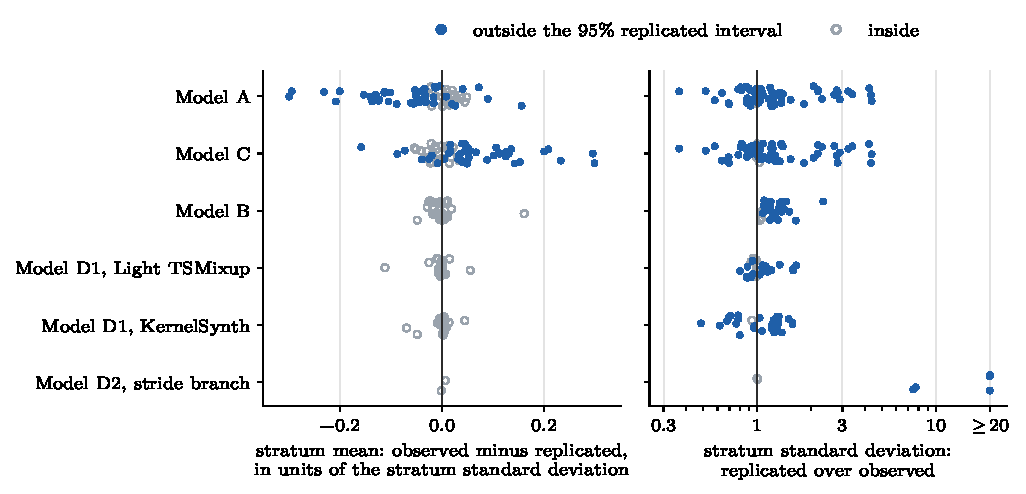
\includegraphics[width=\textwidth]{figures/bayes_ppc_dispersion.pdf}
\caption{Posterior predictive check of every fit that decides a claim, one point per level of every stratum (geometry, candidate frequency, phase slice, $P$, $S$, generator or probe stage as they apply). Left: observed stratum mean minus the centre of its $95\%$ replicated interval, in units of the observed standard deviation of that stratum. Right: centre of the replicated interval of the standard deviation over the observed one, on a logarithmic axis; the Model~D2 levels with an observed standard deviation of zero are drawn at $20$. Filled points fall outside their replicated interval and fail the check. Model~C is fitted on the deficit $-d$, so its mean misses mirror those of Model~A.}
    \label{fig:ppcDispersion}
\end{figure}

The check of Model~A places the stratum means close to the data, with a median miss of $4\%$ of the stratum's standard deviation and at most $30\%$, but $371{,}000$ triplets make every replicated interval a few hundredths wide, so two thirds of the means fall outside. The dispersion misses widely: one residual scale serves every level, while the replicated standard deviation ranges from $0.4$ to $4.4$ times the observed one, the observed spread being smallest at candidate frequencies where the contrast is near zero and largest where the gain is large. The whole response also has a lower median and longer tails than the Student-$t_4$ likelihood reproduces, and Model~C, fitted on the same triplets, fails in the same way. A Gaussian likelihood, fitted as a robustness reading, leaves the pre-gate reading of $H1$ behavioural at refuted and moves the refutation probability of $M1$ from $0.947$ to $0.82$, so the $M1$ reading is the one most sensitive to the model of dispersion that the check rejects.

Models~B and~D1 reproduce every stratum mean and fail on dispersion and on the three quantiles of the whole response: Model~B replicates between $1.0$ and $2.3$ times the observed standard deviation, and Model~D1 between $0.5$ and $1.7$ times. The stride branch of D2 reproduces every mean and the three quantiles, and fails on the standard deviation within each geometry, zero for four of the six and $0.12$ for the other two. The sites fall on the predicted spacing to the step of the grid, while the replicated values carry the resolution floor built into the residual, which no observed scatter below one step can match; the failure is reported because the rule was fixed before the data.

\subsubsection{Readings reported beside the verdicts}

Four readings that decide no claim complete the picture. The contrast formed with the injected amplitude as denominator has mean $0.318$ and median $0.016$, as the fitted one does, and the two differ per triplet with a standard deviation of $0.11$, so the choice of denominator does not move the response. For Model~B, the leave-one-out comparison prefers the form with stage and geometry offsets to the unadjusted one by $255$ units of expected log predictive density, paired standard error $21$, which is why the adjusted form is the primary fit. The realised spread of the eight phase offsets of Model~C is $0.0054$ $[0.0031,0.0076]$, beside a scale $\sigma_\phi$ of $0.006$. And for Model~D1 the stride-only labelling stays within one paired standard error of the two-label fit on both generators, $0.6\pm1.3$ units on KernelSynth and $0.1\pm1.4$ on Light TSMixup, while both lead the patch-only and no-label fits by more than a hundred units, so the patch label adds nothing the stride label does not already carry.

\subsection{Limitations}

Four limitations are properties of the collected design; the first three are reported rather than adjusted for, and the fourth is read through a second fit. The first is the truncated context: every geometry receives $480$ samples, and the $(480-P)\bmod S$ most recent ones, up to sixteen, enter no token (\autoref{tab:sweepContext}). The truncation is identical for a candidate and its two controls, so it cancels within a triplet but not between geometries. It is non-zero on precisely the six runs with $S\nmid P$ that identify the stride branch, so any quantity read across configurations, the covariates of Model~A and the slopes of Model~D2 among them, admits it as an alternative account. The second is the single training seed: a difference between two configurations is also a difference between two trained models, so an effect near a decision threshold may be an artefact of that choice. The third is that the token count $1+\lfloor(L-P)/S\rfloor$ moves with the stride, so the $M1$ slope cannot separate overlap from sequence length, and lowering $S$ also changes the mixture of stride and patch candidates; either confound could produce a slope with no mitigation behind it. The fourth concerns the amplitude $A_{\mathrm{pred}}$ of Model~A: it counts every line the forecast places at the arm's frequency, and the forecasts of the retrained models carry lines of their own on the candidate sites (\autoref{sec:appDecomp}), which would raise $R_k$ and with it $d$, independently of the injected tone. The collection therefore also forecasts every background with no tone, subtracts that forecast's least-squares tone from the arm's as complex coefficients, and refits Model~A on the resulting net contrast. For $H1$ behavioural and $M1$ the net reading must be available, converged and in the same decision class as the primary one, and a disagreement makes the verdict inconclusive.


\flushfloatpages
\appendixsection{The Exploratory Frequency Sweep}{sec:appSweep}
This appendix holds the descriptive pass that precedes the Bayesian analysis. It covers the fifteen geometries of \autoref{tab:hfModels}, five to a figure, and reads each geometry twice: on the left what the model outputs, on the right what its internal state retains. Both readings average over phase, use a single signal family and carry no statement of uncertainty, so they are descriptive and give a high-level view of how frequency content behaves across the geometries. \autoref{fig:rec16-16} in \autoref{sec:results} is the $P=S=16$ row of the same measurement, drawn on its own.

\subsection{How the sweeps are produced}

The measurement is a sweep of pure sinusoids from $2$ to $250$\,Hz in one-hertz steps at $f_s=512$\,Hz, the same band used by the inferential stage, so that the band tasks of \autoref{tab:bandTasks} still partition what is measured. The grid is integer, so the non-integer candidate sites of some geometries, such as $42.\overline{6}$\,Hz for $S=12$ or $21.\overline{3}$\,Hz for $S=24$, are read here at the nearest hertz, whereas the token-collapse sweep of Models~D1 and~D2 and the triplets of Model~A use their exact values (\autoref{sec:appBayes}). Each geometry receives the longest context $L\le512$ that its patch grid covers exactly: $L$ is a multiple of $P$, so Chronos-Bolt adds no masked left padding, and $L-P$ is a multiple of $S$, so every sample enters at least one token, which the model does not guarantee in general because it cuts a patch every $S$ samples from the oldest one. This gives $L=512$ on nine geometries, $504$ on the five with $P=24$ and $496$ on p16-s12 (\autoref{tab:sweepContext}); an integer tone completes a whole number of cycles in the context only at $L=512$, and the resulting leakage is a property of the measurement rather than of the model. \autoref{tab:sweepContext} also reports the tokens and the samples left out of the $480$-sample context of the inferential stage.

The left column is behavioural: the tone is given as context, the median forecast is appended to it and the model is run again, until $512$ samples have been generated; the dominant frequency of that window is the largest magnitude of its discrete Fourier transform after the mean is removed, averaged over up to four starting phases. The window length gives one-hertz bins for every geometry, so a dominant frequency is placed to within a hertz. The loop is imposed from outside, because Chronos-Bolt-Tiny emits its whole horizon in one step, so a curve that degrades along the sweep is partly the model reading its own output, with the error of each step carried into the next.

The right column is representational: at each swept frequency the internal state at the output quantile head is standardised, reduced to its leading twenty principal components, and a logistic regression is trained on that projection and scored by cross-validation, with the standardisation and the projection fitted inside each training fold. Eight tasks are scored per geometry: the seven hierarchical band tasks of \autoref{tab:bandTasks}, after Pagani et al.\autocite{paganiPreliminaryInsightsChronos2026}, which locate a tone by halving the analysed range three times over, and one local task separating a tone at $f-1$\,Hz from one at $f+1$\,Hz. A geometry that answers the first level and fails the third has kept the coarse position of a tone and lost its fine one. The band tasks are cross-validated with folds grouped by frequency, so a probe cannot score by memorising frequencies, while the local task holds out phases, using up to ten per frequency. Because the reduction is unsupervised it may discard low-variance directions that still carry frequency information, and because the probe is linear it scores only what is linearly decodable from the retained components; what is scored is therefore a lower bound on what the state holds, and a red cell shows that a frequency is not easily readable, not that it is absent.

\begin{table}[!htbp]
    \centering
\small
    \setlength{\tabcolsep}{5pt}
    \begin{tabular}{@{}llrrr@{}}
        \toprule
        \textbf{Task} & \textbf{Level} & \textbf{Band [Hz]} & \textbf{Boundary [Hz]} & \textbf{Width [Hz]} \\
        \midrule
        \texttt{Mid} & 1 & $2$--$250$   & $126$ & $248$ \\
        \midrule
        \texttt{L}   & 2 & $2$--$126$   & $64$  & $124$ \\
        \rowsep
        \texttt{H}   & 2 & $127$--$250$ & $188$ & $123$ \\
        \midrule
        \texttt{LL}  & 3 & $2$--$64$    & $33$  & $62$ \\
        \rowsep
        \texttt{LH}  & 3 & $65$--$126$  & $95$  & $61$ \\
        \rowsep
        \texttt{HL}  & 3 & $127$--$188$ & $157$ & $61$ \\
        \rowsep
        \texttt{HH}  & 3 & $189$--$250$ & $219$ & $61$ \\
        \bottomrule
    \end{tabular}
\caption{The seven hierarchical band-classification tasks, after Pagani et al.\autocite{paganiPreliminaryInsightsChronos2026}, each with the level of split it belongs to, the band it is asked of, the boundary that divides that band and the width of the band. The boundaries partition $2$--$250$\,Hz and are held fixed across geometries, so a row may be read across the design.}
    \label{tab:bandTasks}
\end{table}


\begin{table}[!tbp]
    \centering
    \small
    \renewcommand{\arraystretch}{1.1}
    \begin{tabular}{@{}cccccc@{}}
        \toprule
        & & \multicolumn{2}{c}{\textbf{Sweep context}} & \multicolumn{2}{c}{\textbf{$480$-sample context}} \\
        \cmidrule(lr){3-4} \cmidrule(l){5-6}
        \textbf{$P$} & \textbf{$S$} & \textbf{$L$} & \textbf{Tokens} & \textbf{Tokens} & \textbf{Left out} \\
        \midrule
        $8$ & $8$ & $512$ & $64$ & $60$ & $0$ \\
        \midrule
        $16$ & $8$ & $512$ & $63$ & $59$ & $0$ \\
        $16$ & $12$ & $496$ & $41$ & $39$ & $8$ \\
        $16$ & $16$ & $512$ & $32$ & $30$ & $0$ \\
        \midrule
        $24$ & $8$ & $504$ & $61$ & $58$ & $0$ \\
        $24$ & $12$ & $504$ & $41$ & $39$ & $0$ \\
        $24$ & $16$ & $504$ & $31$ & $29$ & $8$ \\
        $24$ & $20$ & $504$ & $25$ & $23$ & $16$ \\
        $24$ & $24$ & $504$ & $21$ & $20$ & $0$ \\
        \midrule
        $32$ & $8$ & $512$ & $61$ & $57$ & $0$ \\
        $32$ & $12$ & $512$ & $41$ & $38$ & $4$ \\
        $32$ & $16$ & $512$ & $31$ & $29$ & $0$ \\
        $32$ & $20$ & $512$ & $25$ & $23$ & $8$ \\
        $32$ & $24$ & $512$ & $21$ & $19$ & $16$ \\
        $32$ & $32$ & $512$ & $16$ & $15$ & $0$ \\
        \bottomrule
    \end{tabular}
\caption{How Chronos-Bolt tokenises the two contexts of this study. A context of $L$ samples is left-padded with masked values to a multiple of $P$ and cut every $S$ samples, so the $(L-P)\bmod S$ most recent samples enter no token (Left out). The sweep uses the longest $L\le512$ with $P\mid L$ and $S\mid(L-P)$; the inferential stage and the decomposition use $480$ samples, which is never padded.}%
    \label{tab:sweepContext}
\end{table}


\begin{figure*}[!p]
    \centering
    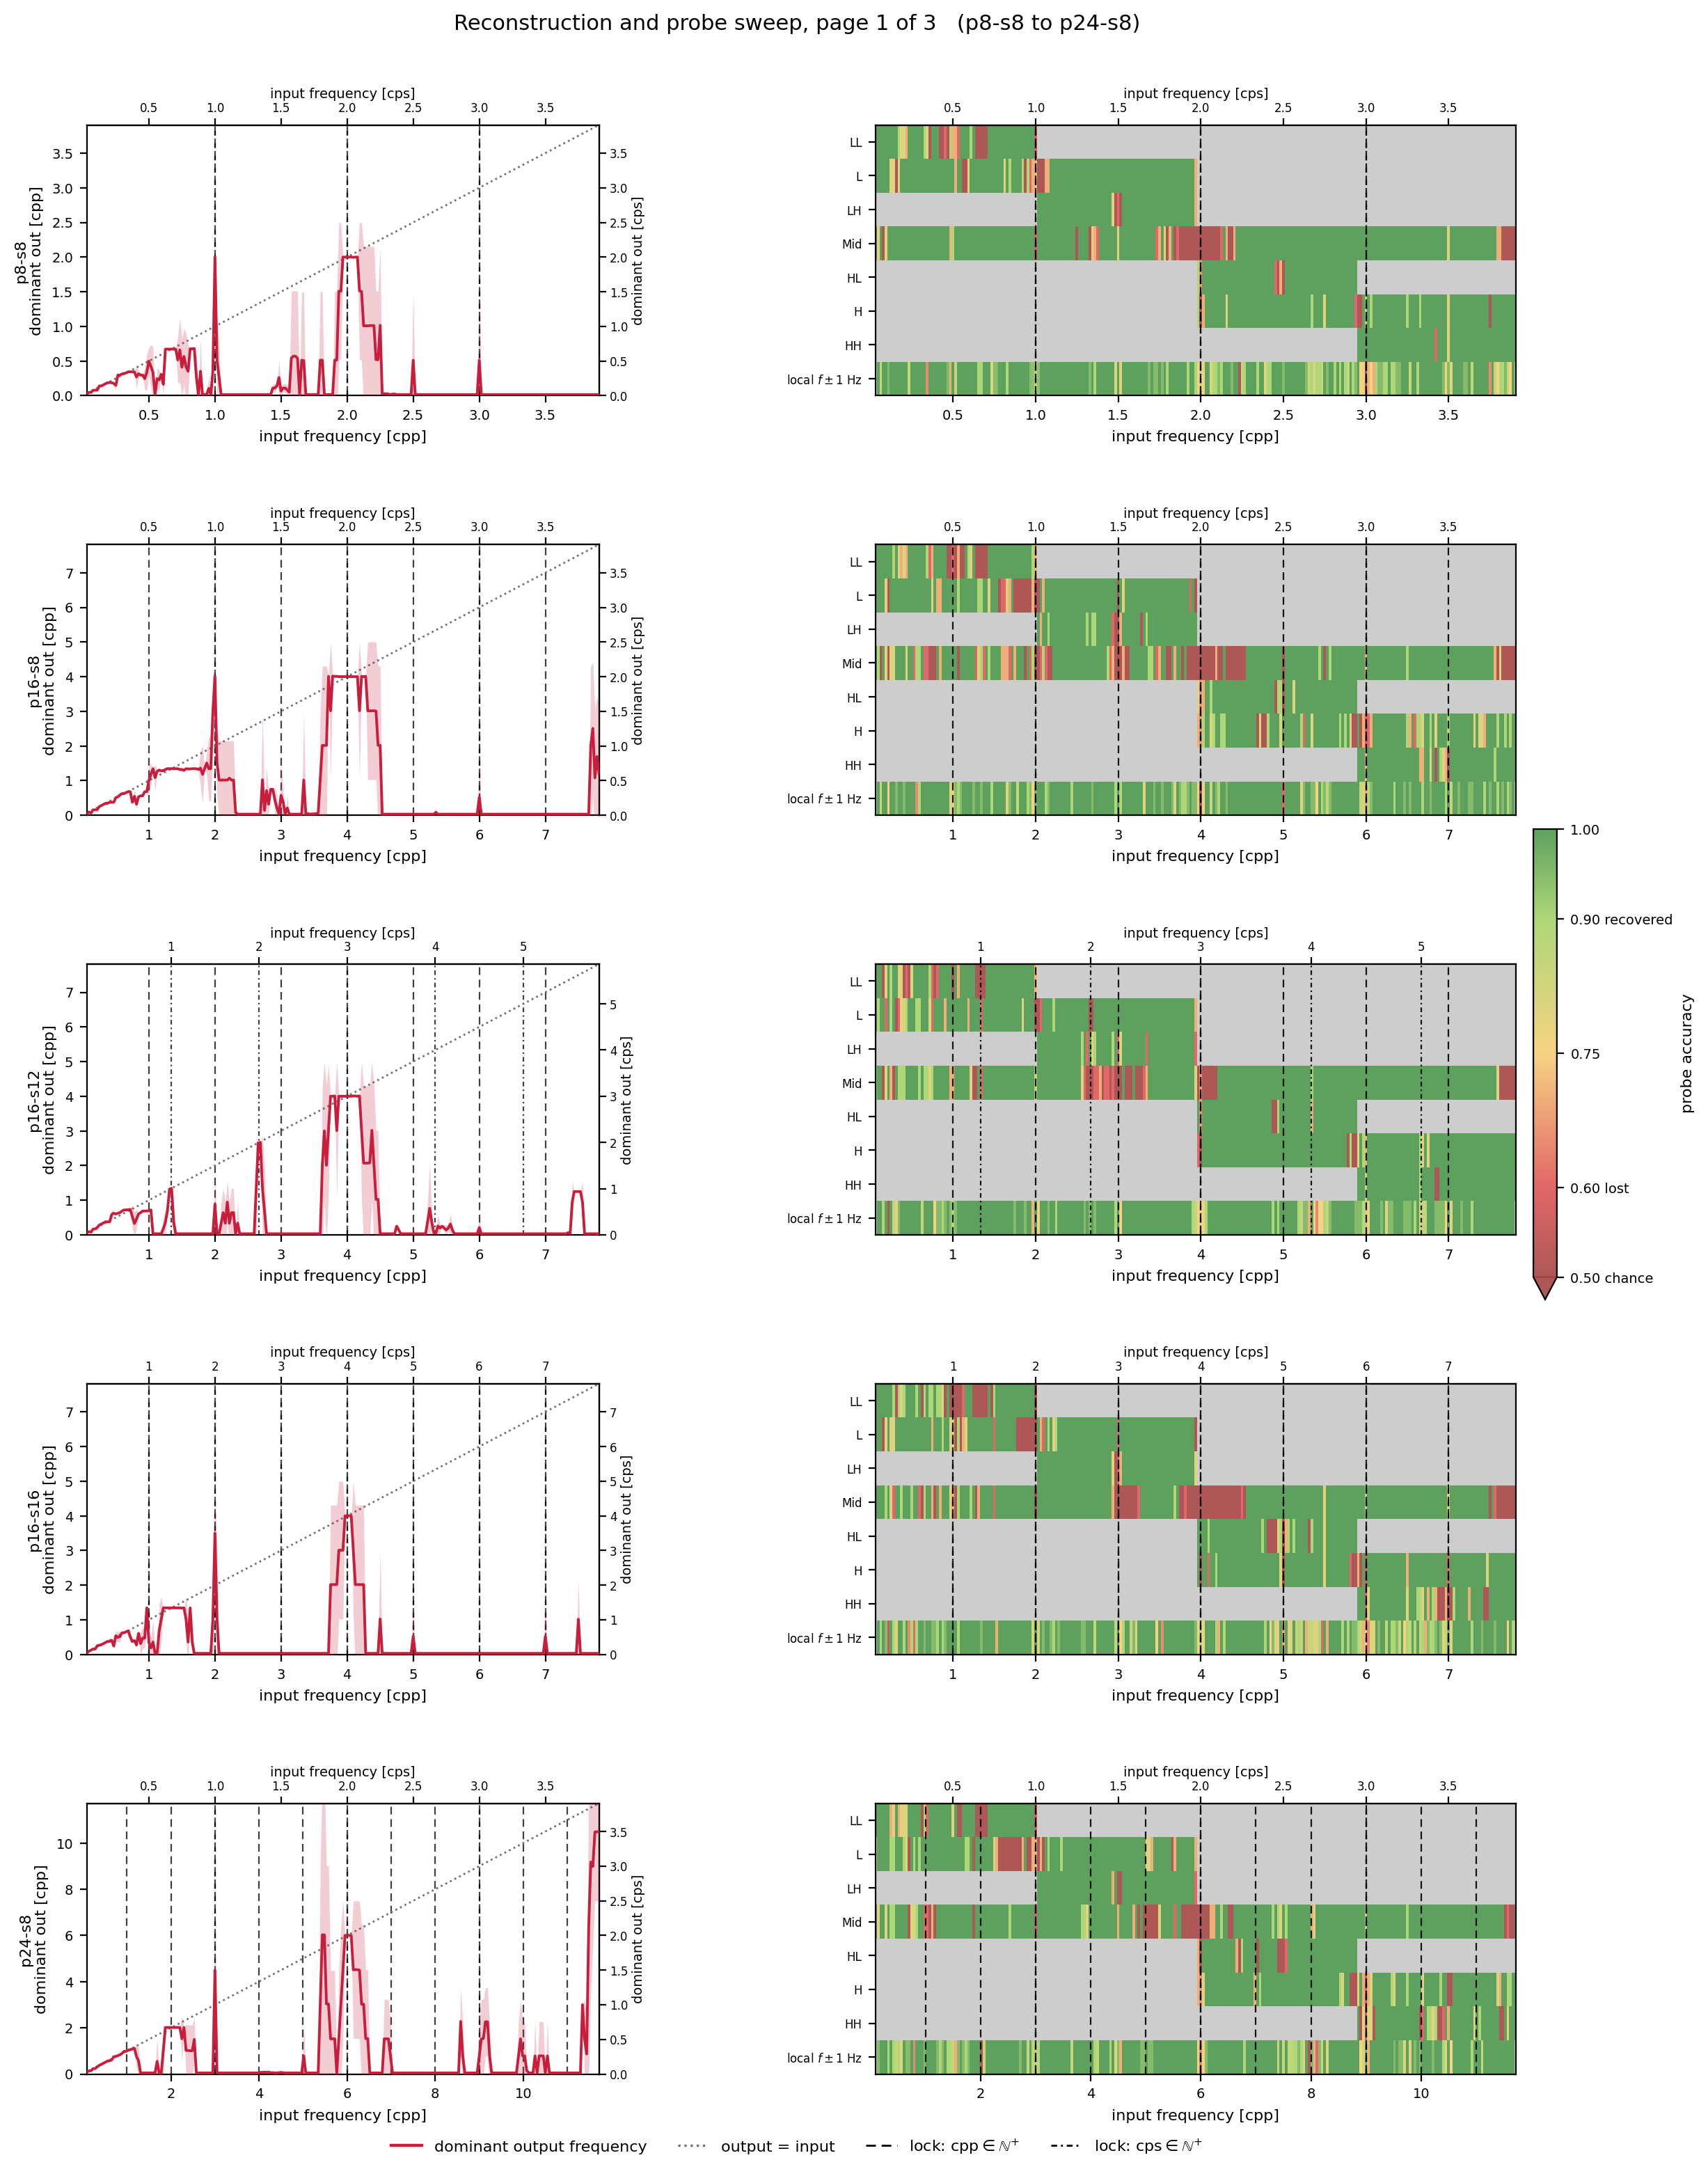
\includegraphics[width=0.8\textwidth]{figures/FIG_E1_page1.png}
    \caption{Reconstruction and probe sweep, first of three: geometries p8-s8, p16-s8, p16-s12,
    p16-s16 and p24-s8. Each row is one geometry. Left, the dominant frequency of the generated
    window against the frequency supplied as context, averaged over up to four starting phases, drawn as
    the solid red curve; both axes are in cycles per patch (bottom and left) and cycles per stride
    (top and right) of that geometry. The pale red band around it is $\pm1$ standard deviation of
    that dominant frequency across the four phases: a wide band at a swept frequency means the
    frequency the model returns depends on where in its cycle the tone began, and a band that
    collapses to the curve means the reading is phase-independent there. The dotted diagonal marks
    a tone rebuilt correctly. Right, the accuracy of a linear probe on the internal state at each
    swept frequency, one strip per task, with the local $f\pm1$\,Hz task last. Dashed verticals
    are that geometry's patch-branch candidates ($\mathrm{cpp}\in\mathbb N^{+}$) and dash-dotted
    verticals its stride-branch candidates ($\mathrm{cps}\in\mathbb N^{+}$). This figure carries
    the two contiguous baselines p8-s8 and p16-s16, the geometries p16-s8 and p24-s8 that share
    $S=8$ with p8-s8, and p16-s12.}
    \label{fig:sweepA}
\end{figure*}

\begin{figure*}[!p]
    \centering
    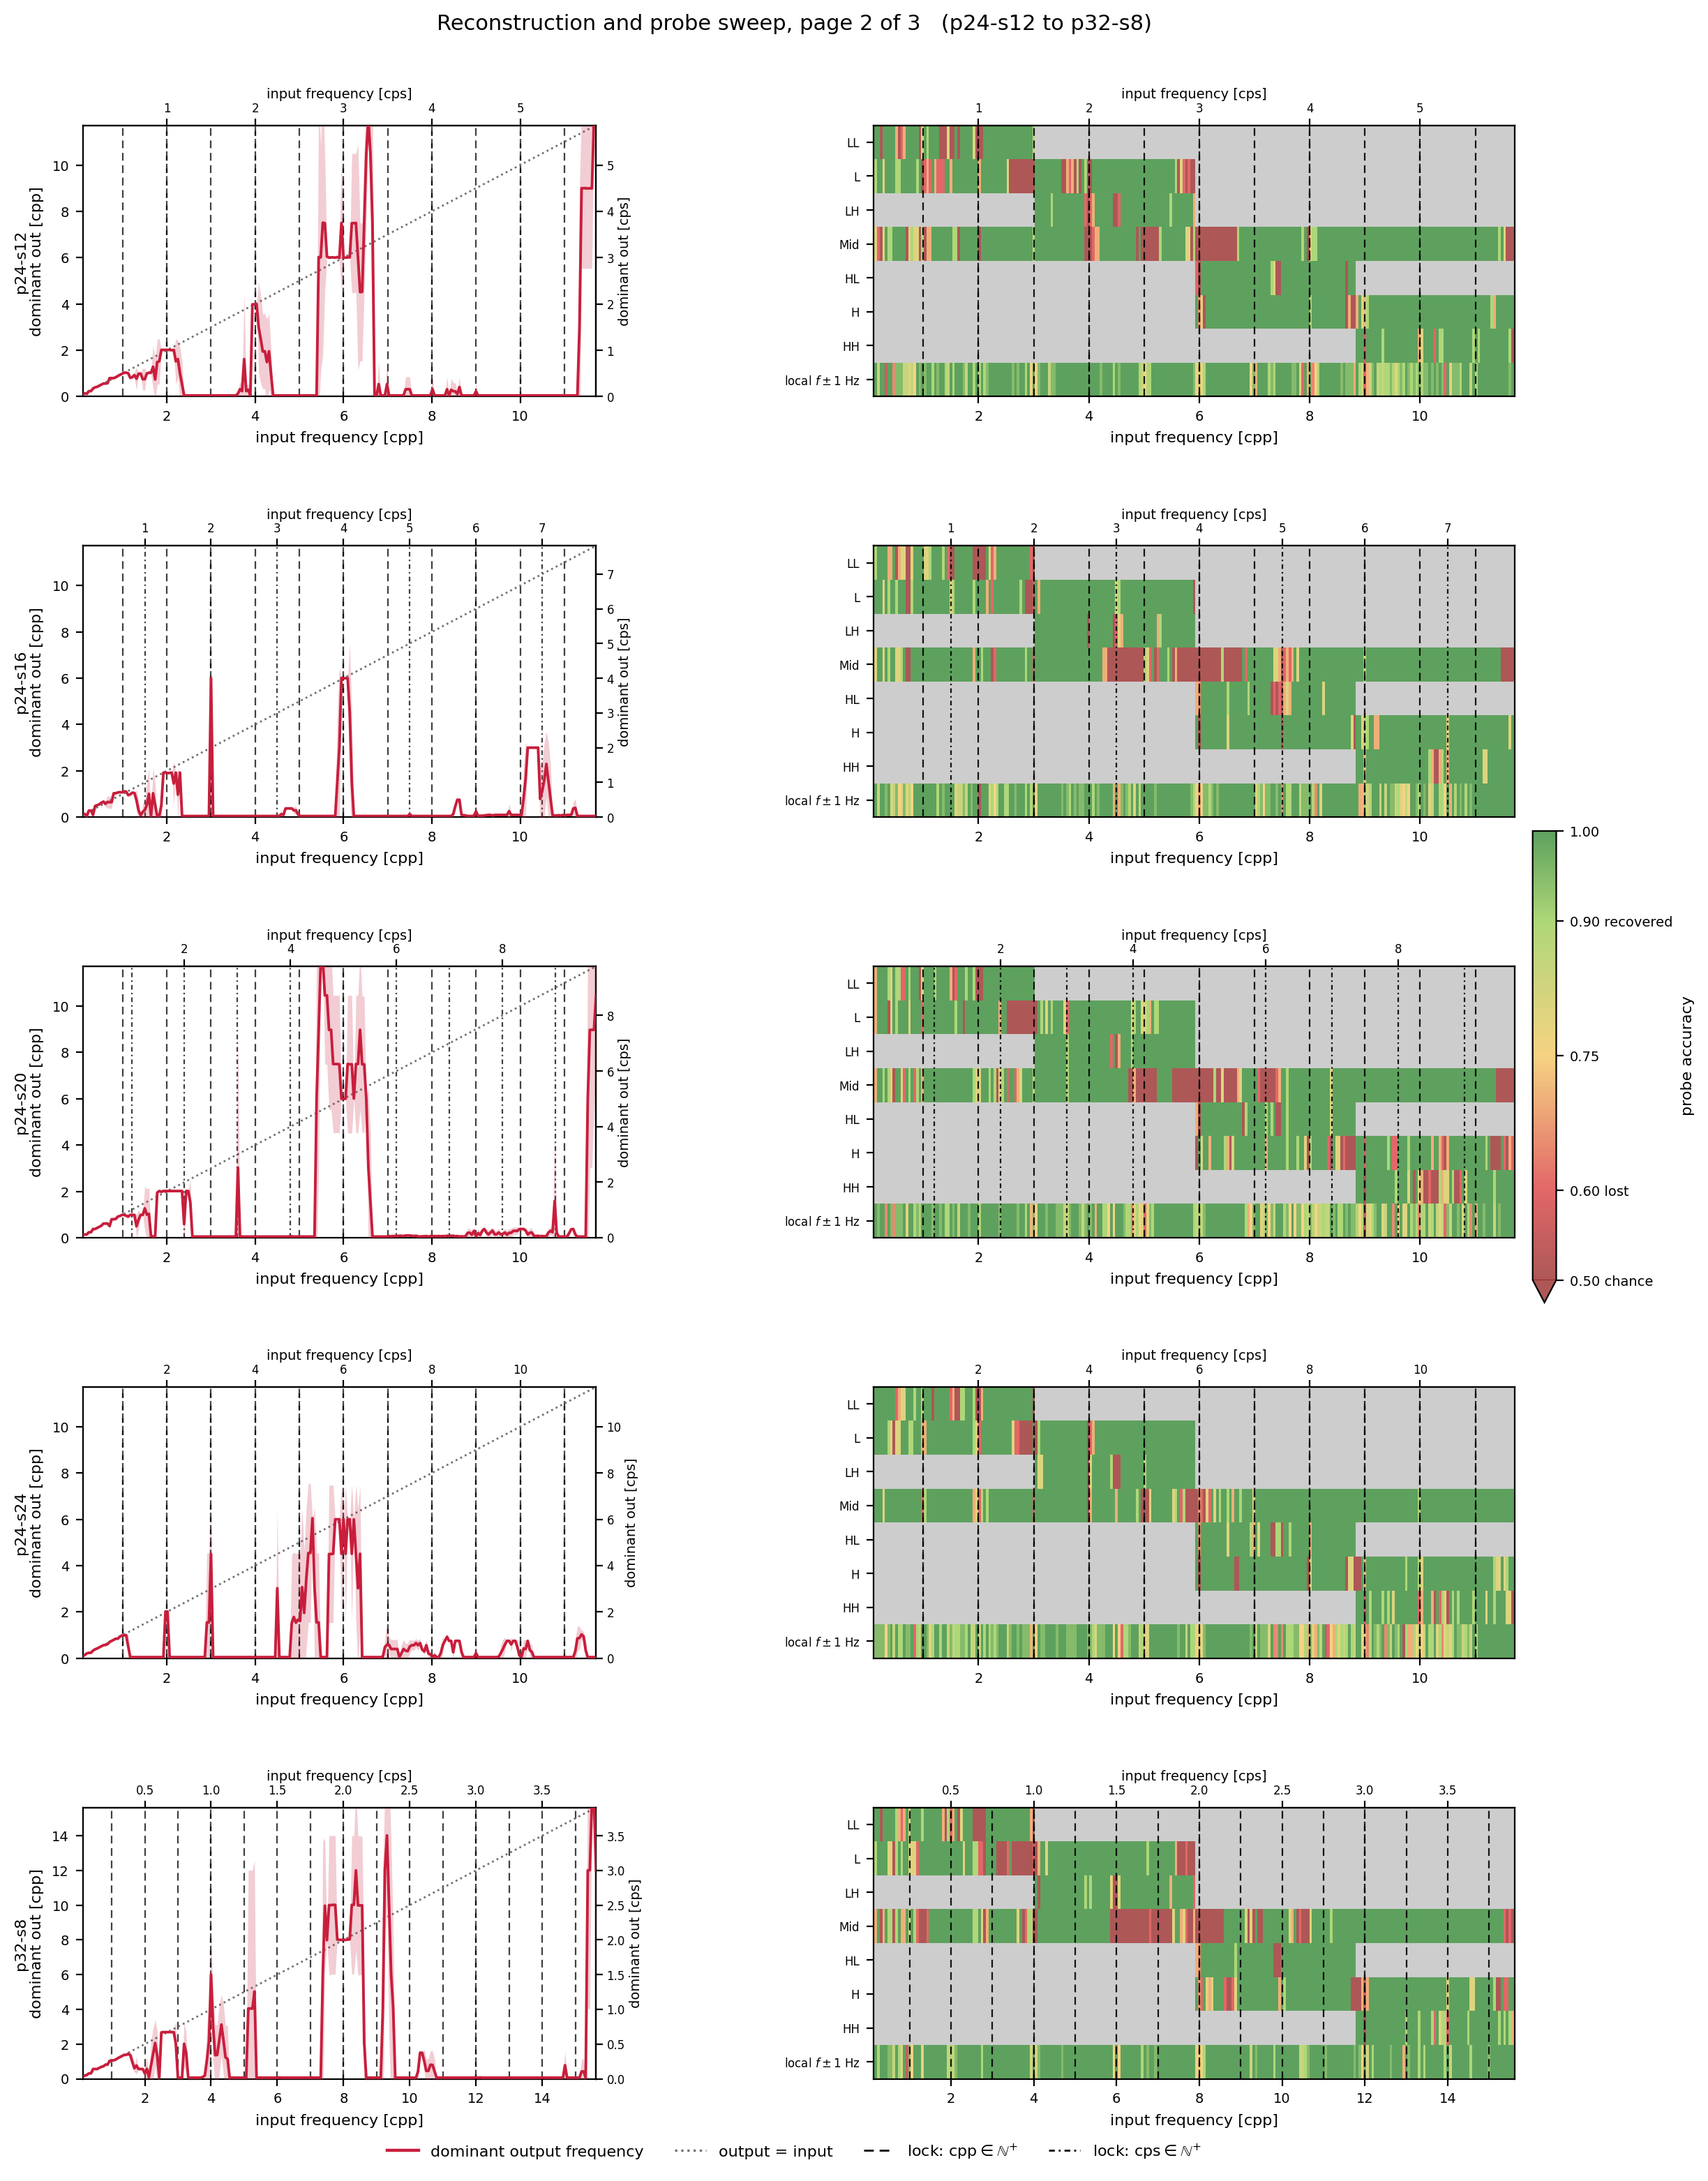
\includegraphics[width=0.85\textwidth]{figures/FIG_E1_page2.png}
    \caption{Second of three: geometries p24-s12, p24-s16, p24-s20, p24-s24 and p32-s8, read as \autoref{fig:sweepA}. The first four hold the patch size at $P=24$ and shorten the stride
    from $24$ to $12$, so the stride comb $c f_s/S$ moves across the band while the patch comb
    $k f_s/P$ stays where it is: this is the series on which the two branches of
    $\mathcal F_{\mathrm{lock}}$ can be told apart by eye, and p24-s16 and p24-s20 are among the
    six runs with $S \nmid P$ on which the branch estimates of \autoref{sec:models} rest.}
    \label{fig:sweepB}
\end{figure*}

\begin{figure*}[!p]
    \centering
    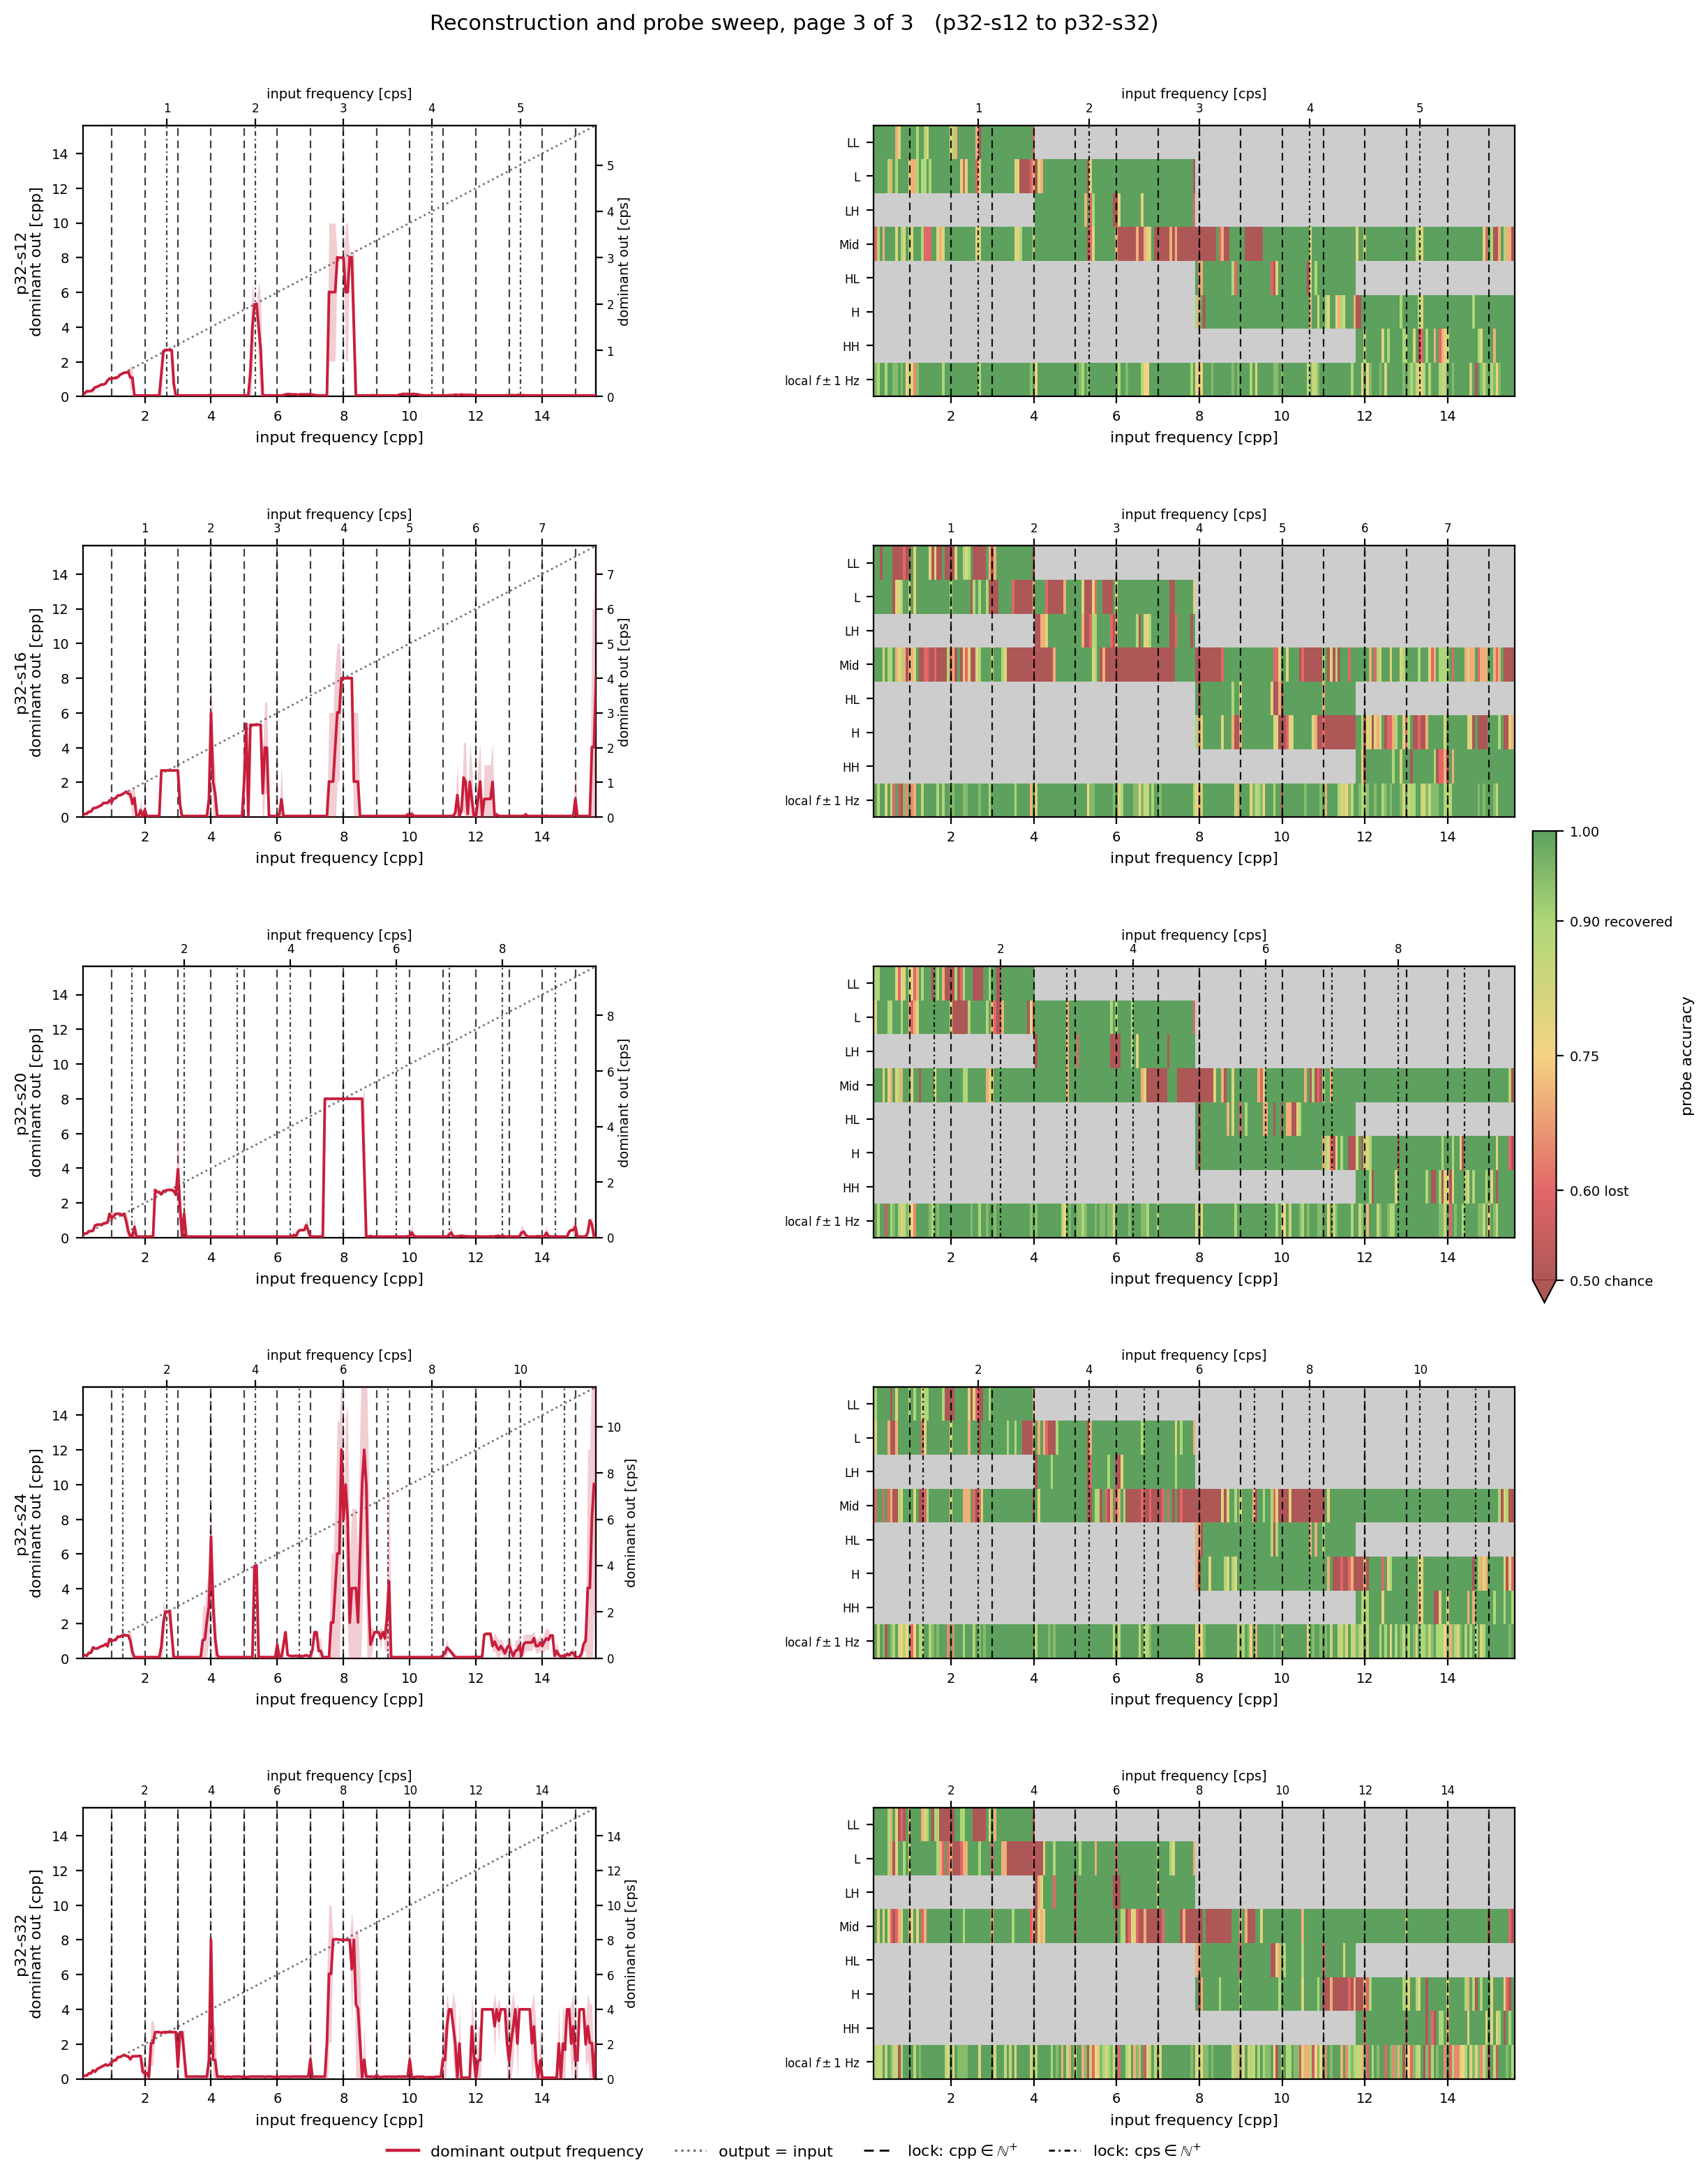
\includegraphics[width=0.85\textwidth]{figures/FIG_E1_page3.png}
    \caption{Third of three: geometries p32-s12, p32-s16, p32-s20, p32-s24 and p32-s32, read as \autoref{fig:sweepA}. The patch size is held at $P=32$, the widest of the design, so the
    patch comb is the densest and the overlap ratio runs from $0.63$ down to $0$ within this one figure.
    Read against \autoref{fig:sweepB} at equal stride, the difference between the two is a difference of
    patch size alone, which is the comparison the covariate $\log P$ of \autoref{eq:appM1:model}
    is fitted to.}
    \label{fig:sweepC}
\end{figure*}

\subsection{What is shown for each geometry}

Figures~\ref{fig:sweepA}, \ref{fig:sweepB} and~\ref{fig:sweepC} divide the design by patch size. The first carries the two smallest patches and the first $P=24$ run, where the combs are coarsest; the second completes the $P=24$ series and opens the $P=32$ block, the range over which stride varies at fixed patch size; the third holds the five $P=32$ geometries, where the patch comb is densest, ending on $P=S=32$, where the two branches coincide.

On the left, a point on the dotted diagonal is a tone rebuilt at the frequency it was given. A flat segment means that distinct inputs return dominant frequencies in the same bin, a loss of distinguishability rather than of amplitude, and a jump is a tone the model produces that was never supplied. The shaded band is one standard deviation over the starting phases. On the right, each cell is one swept frequency coloured by probe accuracy on a continuous scale, green at or above $0.9$, yellow near $0.75$ and red below $0.6$, close to chance; grey marks a frequency no task covers. Every axis is in cycles per patch and cycles per stride of the geometry drawn, so a candidate site falls on an integer of one of the two scales. The dashed and dash-dotted verticals are the candidate sites $\mathcal F_{\mathrm{lock}}$ of the patch and stride branches, computed from $(f_s,P,S)$ and not fitted. A frequency off the diagonal on the left but green on the right was lost between the representation and the output, not at the tokenisation, while a red cell means the internal state itself no longer separates that frequency from its neighbour.

\subsection{What the figures show}

The reconstruction follows the diagonal only up to roughly one cycle per patch, and above it the output is mostly a slow component unrelated to the input: the dominant output lies within $2$\,Hz of the input for $7$ to $15\%$ of the swept tones, depending on the geometry. The exceptions are tied to particular frequencies rather than scattered. At most geometries a plateau returns the inputs near $f_s/4$ at $f_s/4$ itself, which lies at $2$, $4$, $6$ and $8$\,cpp for $P=8$, $16$, $24$ and $32$ and is a patch-branch site of every geometry. Narrow spikes appear mostly at inputs lying on a site of either branch, where the output leaves the slow component and jumps, often to another site, while the neighbouring inputs do not; on p24-s20 one falls on a stride-branch site at $3$\,cps. The phase band is widest on the plateaus, so where many inputs collapse onto one output the collapse also depends on the starting phase.

The probe strips do not follow that pattern. The local task stays at or above $0.9$ over most of the band, $66$ to $91\%$ of it by geometry and least at p32-s32, including at frequencies the reconstruction no longer places, with yellow cells that become denser towards the top of the band rather than at the sites. The band tasks are weaker, and their red cells gather at the low end of the band and beside the task boundaries of \autoref{tab:bandTasks}, most visibly in the Mid and L tasks. The boundaries of the first two levels lie next to $f_s/8$, $f_s/4$ and $3f_s/8$, sites of every geometry, and those of the third next to odd multiples of $f_s/16$, sites for $P=16$ and $P=32$, so on this design the difficulty a band task has at its own boundary cannot be told apart from an effect of the site.

These readings are descriptive, since neither is paired against controls or carries an interval. They show that the two readings disagree in a specific direction, a frequency still separated in the internal state and misplaced in the output, and that on the output the sites act as attractors rather than as holes. That observation gives the study its direction, and the Bayesian hypotheses reported in \autoref{sec:bayesResults} test it.


\flushfloatpages
\appendixsection{Decomposition of Generated Signals}{sec:appDecomp}
This appendix states how the decomposition reading of \autoref{sec:results} is produced. It moves the question of \autoref{sec:appSweep} from pure tones to realisations of the two generators of \autoref{sec:signals}, and it has two outputs: single draws, in which a real window and the forecasts made from it are split into their frequency components and set side by side, and a recovery count over many draws, which is what \autoref{tab:decomposition} summarises. Both are descriptive and serve to show which frequency components the models appear unable to return, giving the study a direction that the Bayesian hypotheses then test rather than a verdict of their own. Neither is paired against a matched control in the sense of \autoref{sec:framework}, and neither carries a statement of uncertainty.

\subsection{Signals and forecasts}

A realisation is drawn from one of the two generators and normalised to unit variance. Light TSMixup follows \autoref{sec:appTSMixup} with two changes made for this reading: the number of components is drawn between one and four rather than up to ten, and no two drawn frequencies may lie closer than $10$\,Hz, so that every component can be told apart at the resolution the horizon allows. KernelSynth follows \autoref{sec:appKernelSynth} with at most five kernels per draw, and in both cases the first $480$ samples are supplied as context and the following $64$ are kept as the real continuation.

The same context is given to two checkpoints: a retrained geometry of \autoref{tab:hfModels} and the published Chronos-Bolt-Tiny, which is itself $P=S=16$ but was trained with a larger budget and a recipe that is not fully published (\autoref{sec:appRetraining}). Each returns its native $64$-sample horizon in a single pass, and the median quantile is kept. Nothing is fed back into the context, so the reading concerns the forecast a deployment actually receives rather than the rollout of \autoref{sec:appSweep}. The real continuation covers the same $64$ instants as the two forecasts, so the three windows share their length, their position in time and their resolution, and a difference between them is not a difference of window.

\subsection{From a window to its components}

Each of the three windows is decomposed in the same way. Its mean is removed, it is multiplied by a Hann window, and its one-sided magnitude spectrum is computed and scaled so that a pure tone of amplitude $A$ peaks near $A$. The spectrum is evaluated on a one-hertz grid obtained by zero padding, which places a peak finely but does not separate two peaks: the native spacing remains $f_s/64=8$\,Hz, and two components closer than that appear as one line however fine the grid.

Candidate lines are the local maxima of that spectrum inside the analysed band of $2$--$250$\,Hz, taken strongest first, no two closer than the native spacing, and none weaker than $5\%$ of the strongest. Up to six are kept on the real side and up to eight on each forecast. On the real side of a Light TSMixup draw the lines are not estimated at all, since the generator records the frequencies it used; a KernelSynth draw names no frequencies, so its real side is read off the spectrum like the forecasts. A forecast line is then retained only if its magnitude reaches $35\%$ of the strongest candidate of the same forecast. The cut is computed separately for each checkpoint, so a forecast that is weak overall is not emptied by a threshold set on another model's output.

Retained lines are turned into components by one joint least-squares fit over the window: a sinusoid at every retained frequency plus a constant, fitted together so that energy shared by two nearby frequencies is split between them instead of being counted twice. The fit returns an amplitude and a phase per line; it never adds or removes a line, which is decided by the spectrum alone. A component whose frequency completes fewer than one and a half cycles in the window is flagged, since below that an amplitude cannot be separated from a phase, and a fit that is poorly conditioned is reported as such rather than returned as a clean number.

\subsection{Reading the figures}

Each draw produces two pages, and the components page has three columns, the real continuation, the retrained geometry and the published checkpoint, each headed by its own window. Below the window each row is one component, drawn over the same absolute time interval and titled with its frequency in hertz, in cycles per patch and in cycles per stride of that column's own geometry, and with its fitted amplitude $A$; a component within one hertz of a candidate site of that geometry is marked as such. Every component panel of a page shares one vertical scale, set by the strongest real component, so a forecast line at a few per cent of the input reads as small rather than being enlarged to fill its box.

The spectra page draws the three magnitude spectra in the same order, each with cycles per patch on the lower axis and cycles per stride on the upper one, both computed with that panel's geometry. Dashed verticals are the candidate sites $\mathcal F_{\mathrm{lock}}$ of that geometry, grey margins lie outside the analysed band, the dotted horizontal is the $35\%$ cut, and triangles mark exactly the lines carried into the components page. On a Light TSMixup draw a green vertical marks each frequency the generator drew.

\subsection{Single draws}

\autoref{fig:decompKS} to \autoref{fig:decompTSlowspec} show three draws at the reference geometry $P=S=16$, one KernelSynth background and two Light TSMixup ones, each forecast by the retrained model and by the published checkpoint, with the components of a draw on one page and the spectra they were read from on the next. They are illustrative: they show how the two checkpoints behave on individual signals, test no hypothesis and are not samples in any statistical sense, while the aggregate over many draws is \autoref{tab:decomposition} in \autoref{sec:results}.

Frequencies below are in cycles per patch, equal to cycles per stride at this geometry, and the native spacing of the $64$-sample window is $0.25$\,cpp. The KernelSynth draw carries six lines spread over the whole band, at $1.38$, $2.66$, $3.56$, $4.41$, $5.34$ and $7.56$\,cpp. The published checkpoint recovers more of them: it returns lines at $2.66$ and $5.34$\,cpp, one at $3.38$\,cpp that lies within the native spacing of the $3.56$\,cpp line, and slow content at $0.34$ and $0.66$\,cpp, beside a line at $4$\,cpp. The retrained model keeps only two lines, a slow one at $0.59$\,cpp and one at $4$\,cpp; that line sits on a candidate site of the geometry, between the real lines at $3.56$ and $4.41$\,cpp rather than on either of them, and neither checkpoint returns the highest line.

\begin{figure*}[p]
    \centering
    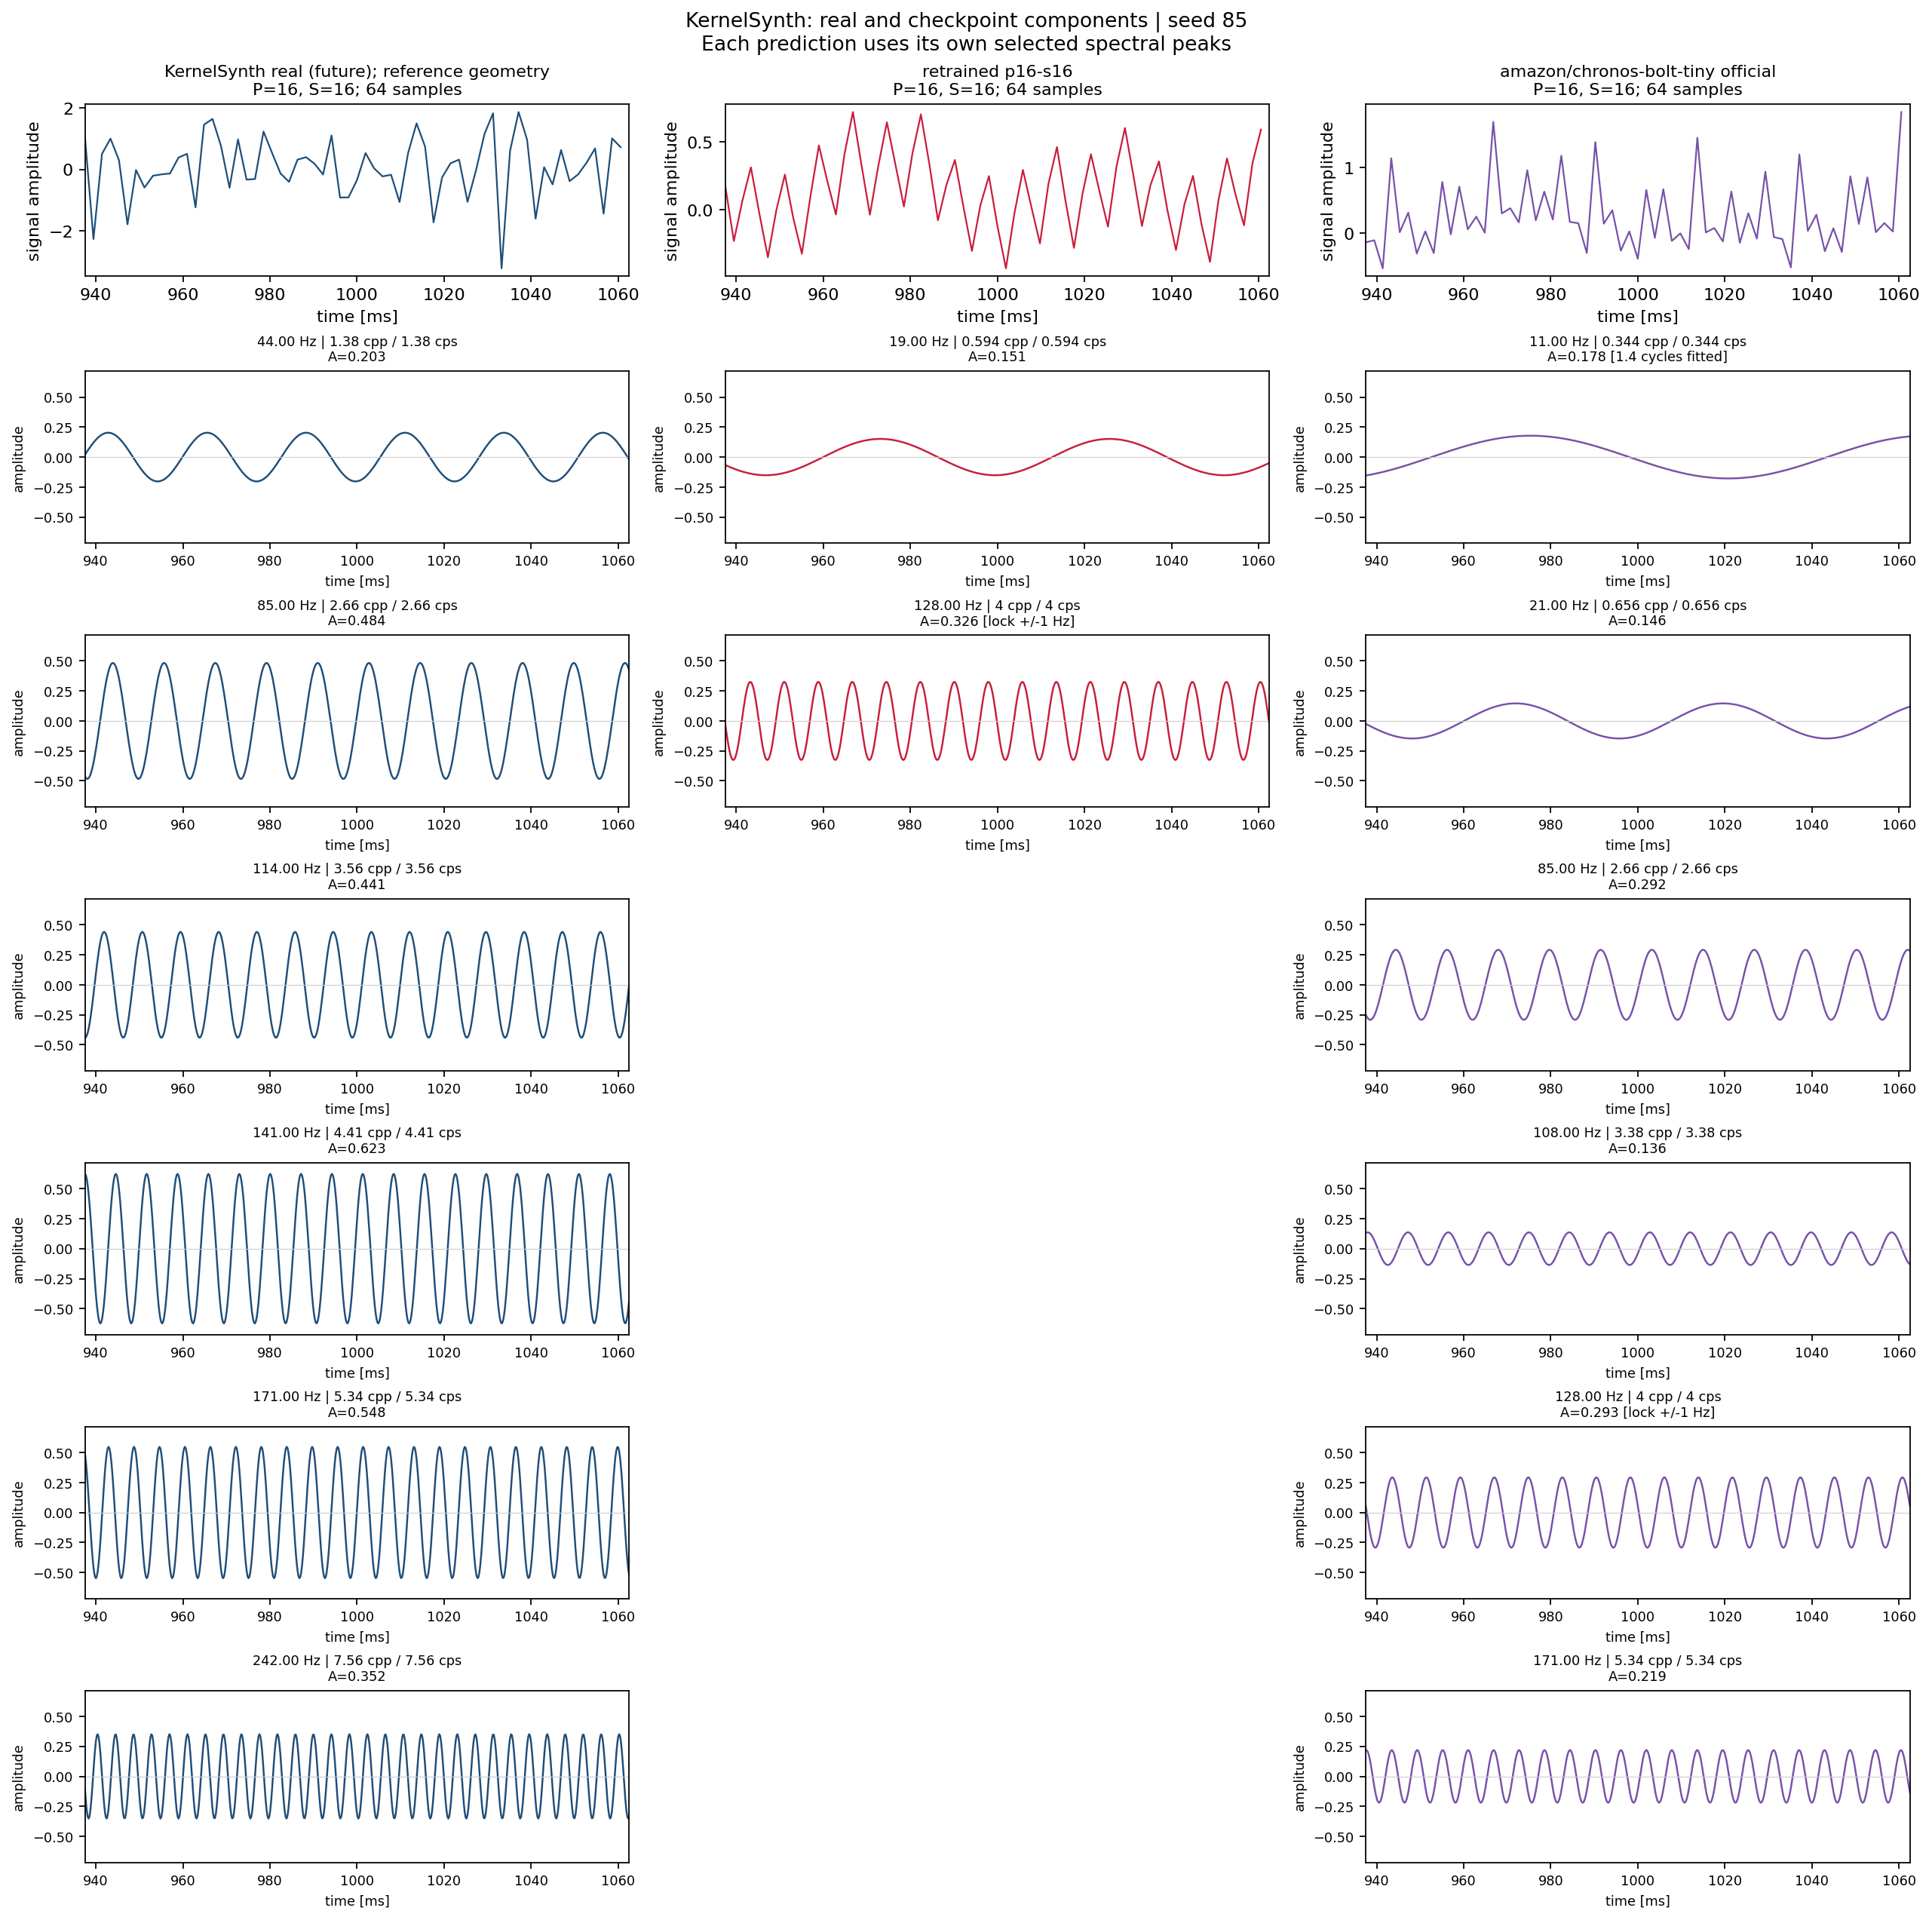
\includegraphics[width=\textwidth,height=0.86\textheight,keepaspectratio]{figures/FIG_G_kernelsynth_p16-s16_seed85_components.png}
\caption{KernelSynth draw at the reference geometry $P=S=16$, components. Columns, left to right: the real continuation, the forecast of the retrained model and that of the published checkpoint, each headed by its $64$-sample window; each row below is one retained component, titled with its frequency in hertz, in cycles per patch and per stride, and its fitted amplitude, and marked when it lies within one hertz of a candidate site. Both sides are estimated, since the generator names no frequencies. Illustrative only: the aggregate is \autoref{tab:decomposition}.}
    \label{fig:decompKS}
\end{figure*}

\begin{figure*}[p]
    \centering
    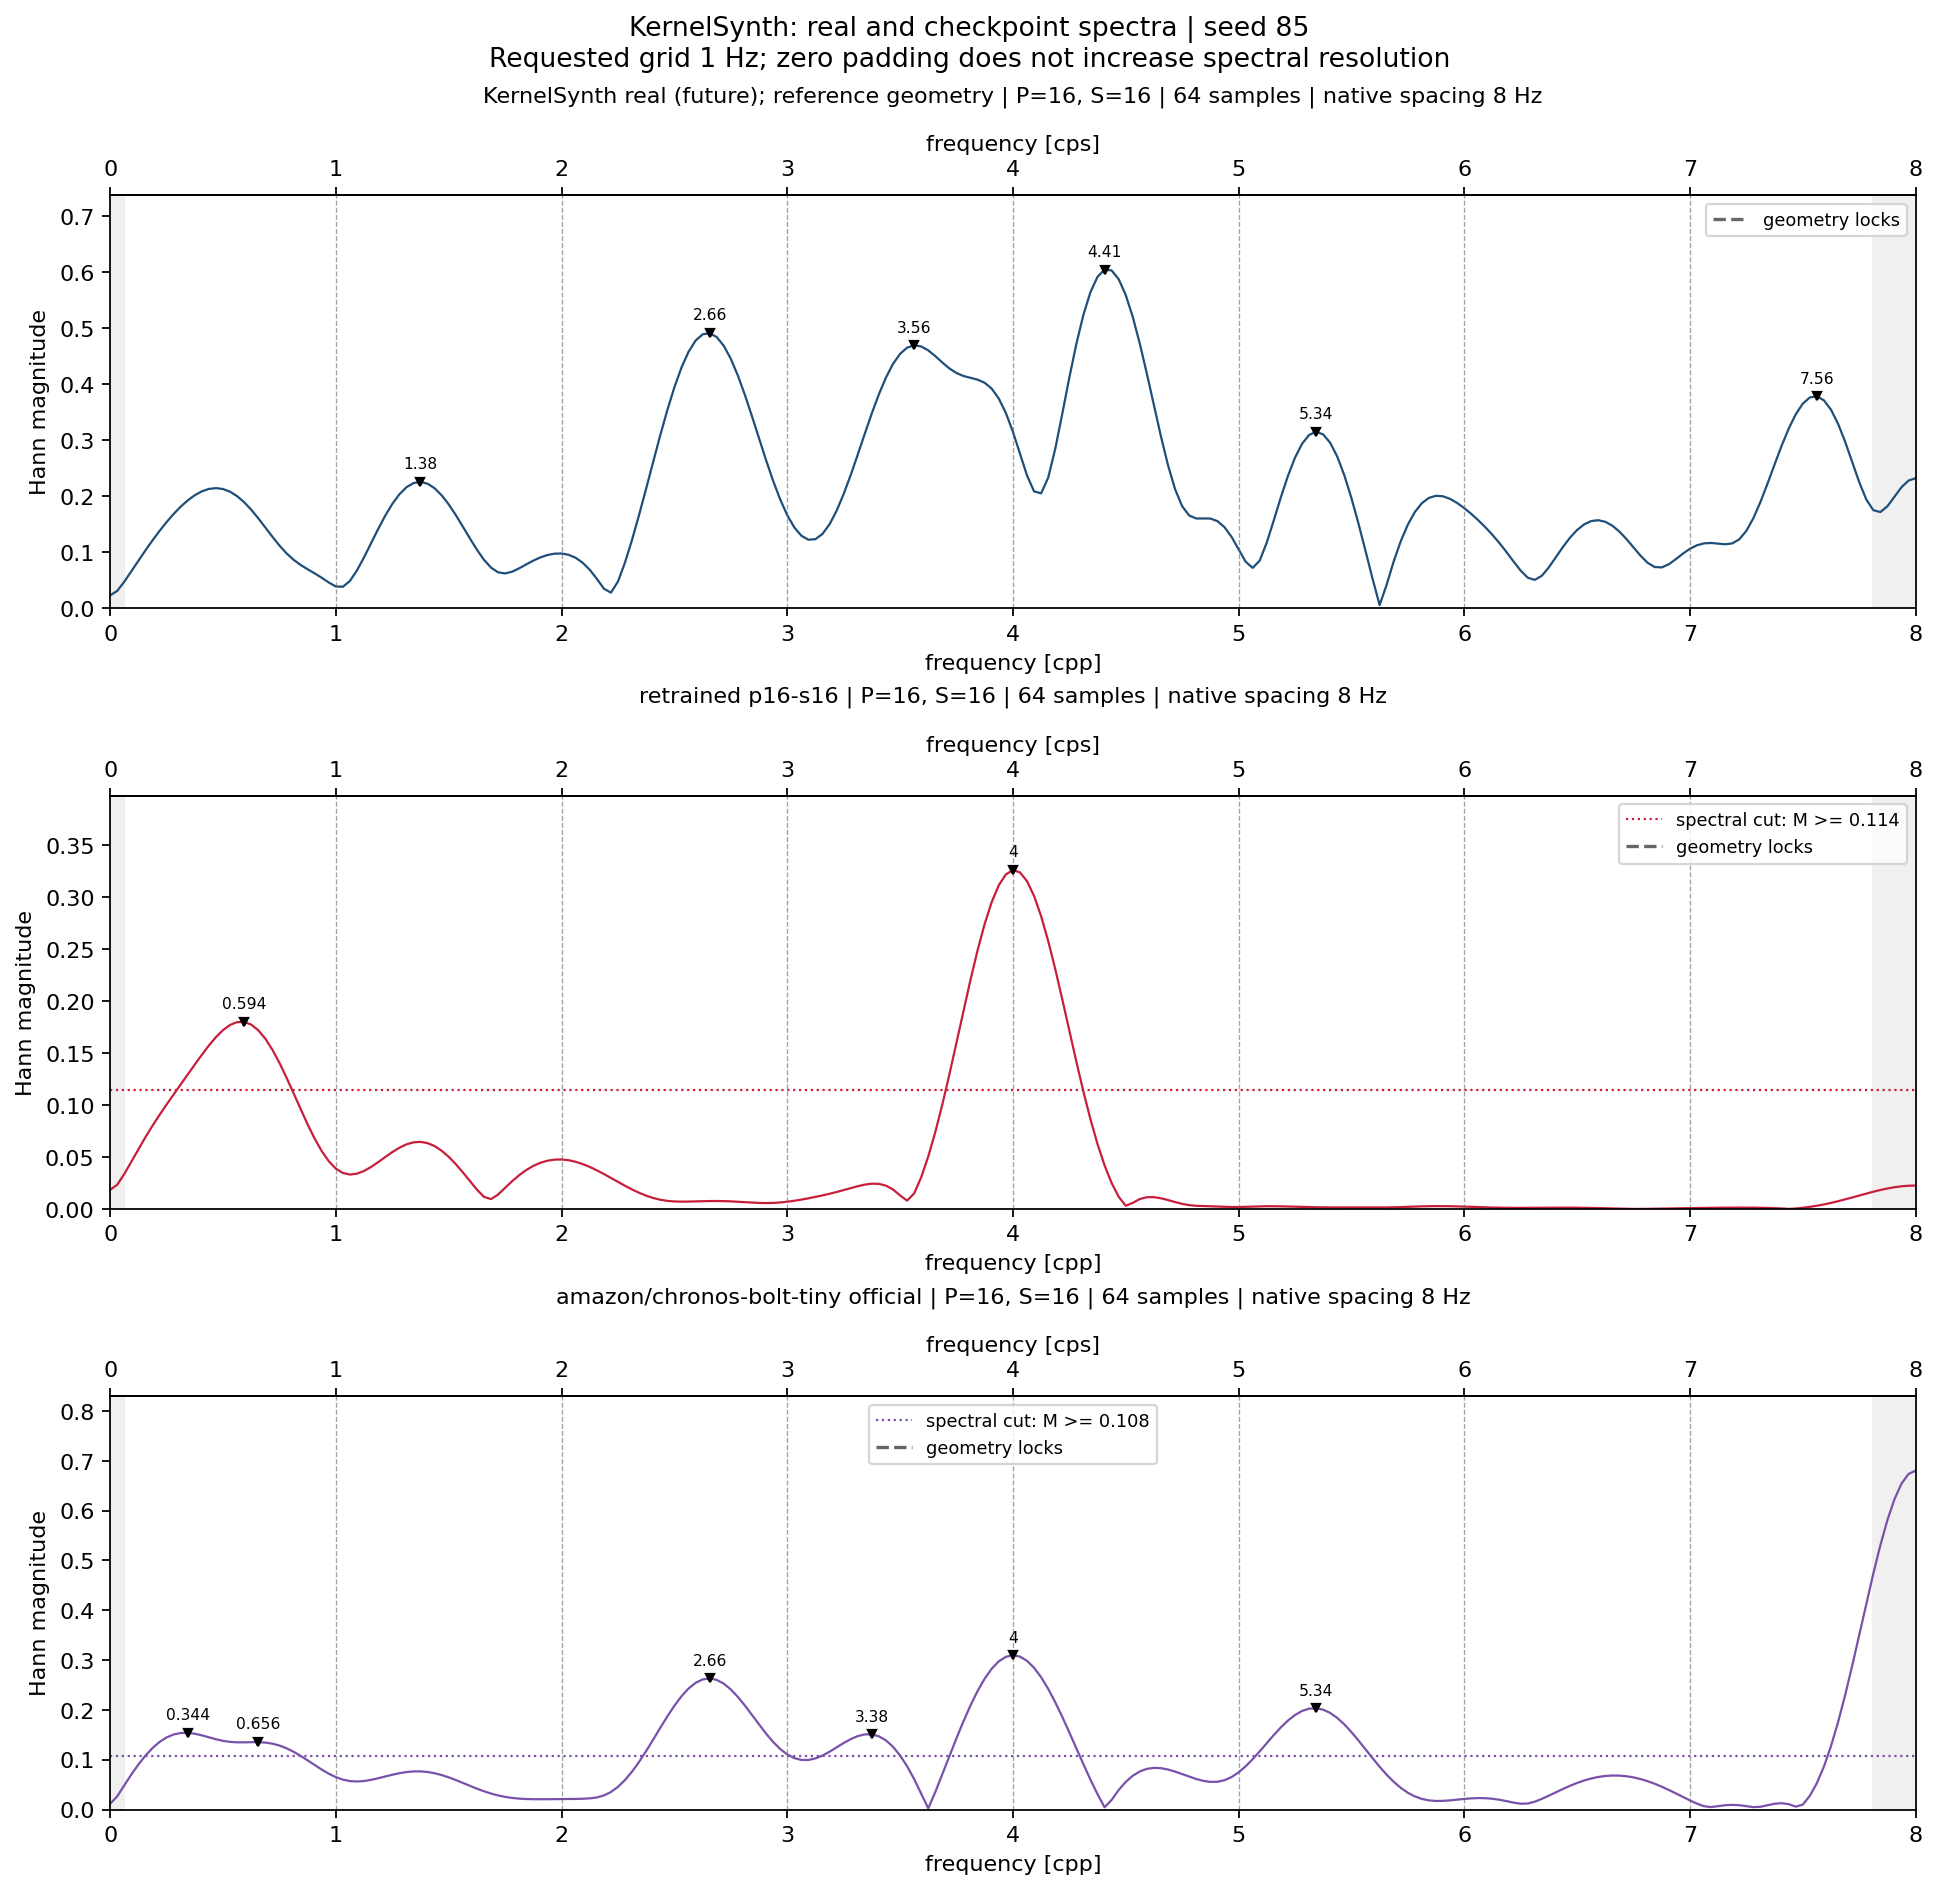
\includegraphics[width=\textwidth,height=0.80\textheight,keepaspectratio]{figures/FIG_G_kernelsynth_p16-s16_seed85_spectra.png}
\caption{Spectra of the draw of \autoref{fig:decompKS}: real continuation (top), retrained model (middle) and published checkpoint (bottom), in cycles per patch on the lower axis and per stride on the upper one. Dashed verticals are the candidate sites, the dotted horizontal is the $35\%$ cut and triangles mark the lines carried into the components page; grey margins lie outside the analysed band.}
    \label{fig:decompKSspec}
\end{figure*}

The first Light TSMixup draw carries a single injected tone at $6.16$\,cpp with amplitude $1.42$, and neither checkpoint returns it. Both forecasts are nearly flat, their strongest lines are two orders of magnitude weaker than the input, and two of the retrained model's residual lines fall on its own candidate sites at $2$ and $4$\,cpp, the second within $0.03$\,cpp. The second draw injects a tone at $1.30$\,cpp into a background that already holds a component at $6.69$\,cpp. Both checkpoints keep the injected tone, returning it at $1.34$\,cpp, within the native spacing, with amplitude close to the input for the retrained model ($1.06$ against $1.08$) and somewhat lower for the published one ($0.84$). Both lose the high component that was already in the signal, and a weak line at $0.88$\,cpp falls below the cut in either forecast.

\begin{figure*}[p]
    \centering
    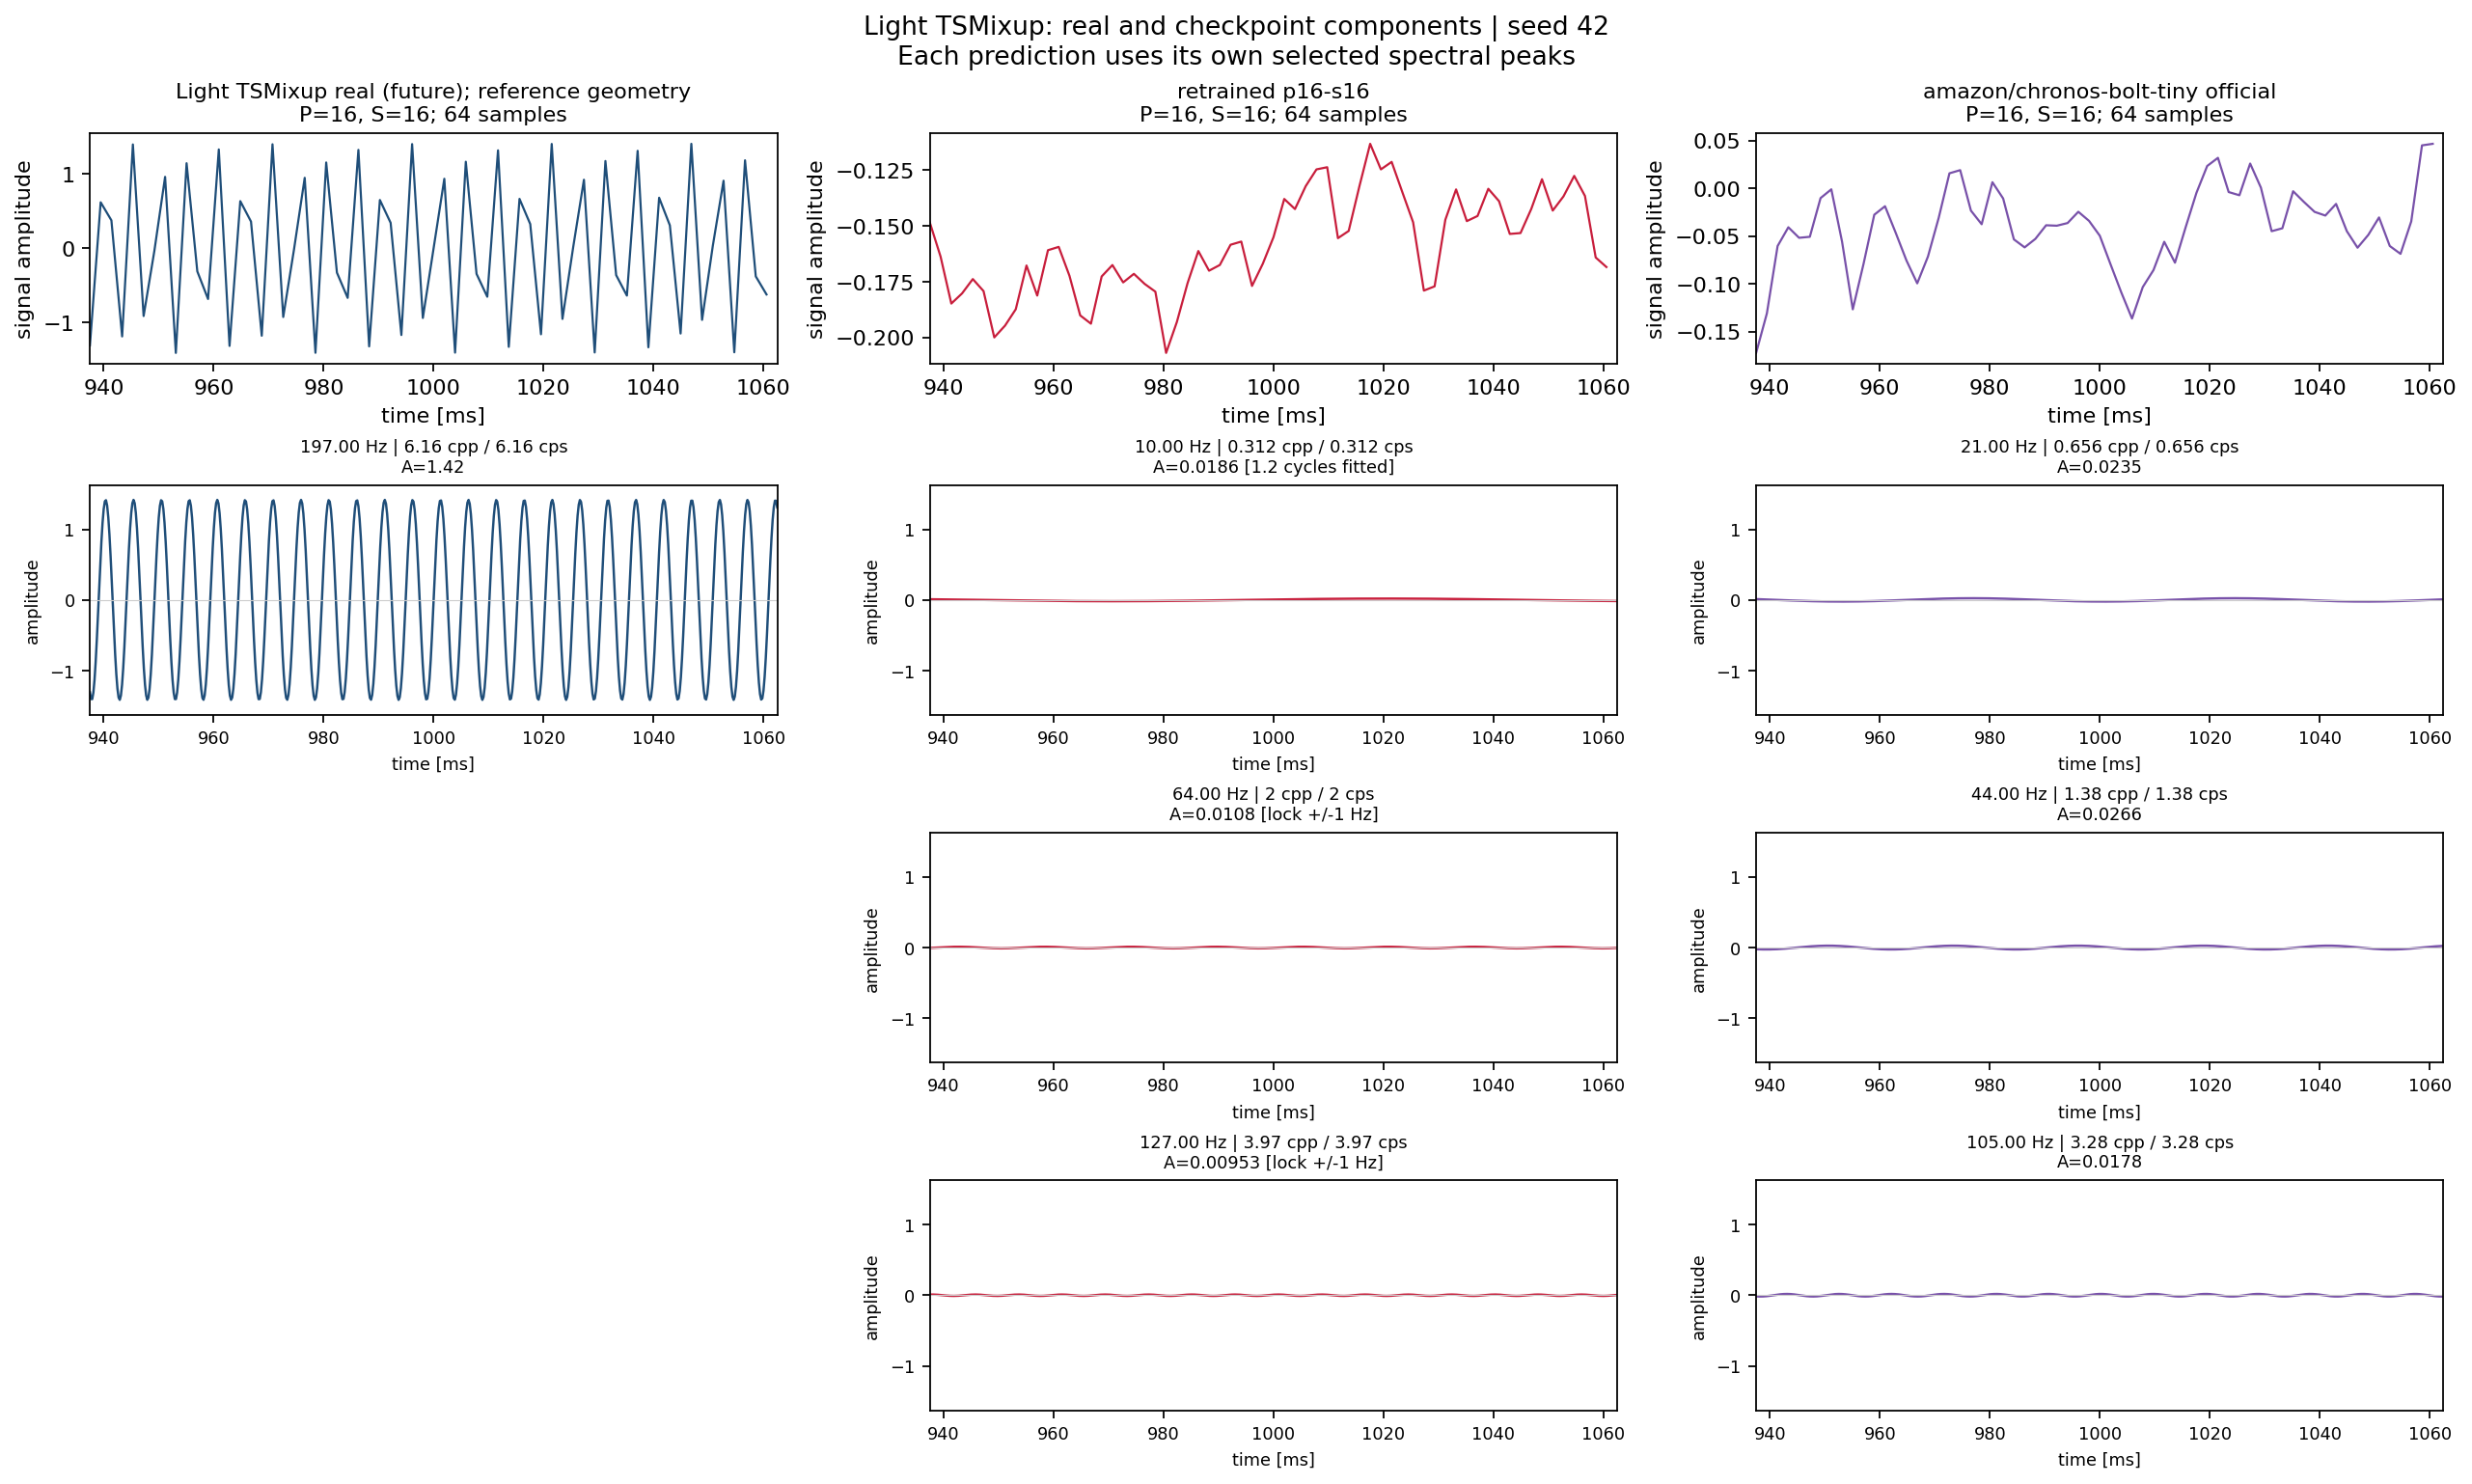
\includegraphics[width=\textwidth,height=0.70\textheight,keepaspectratio]{figures/FIG_G_tsmixup_p16-s16_seed42_components.png}
\caption{Light TSMixup draw with a single high-frequency injected tone at $6.16$\,cpp, reference geometry $P=S=16$, components, read as \autoref{fig:decompKS}. The real side lists the frequencies the generator drew rather than estimating them. Every component panel shares the vertical scale of the strongest real component, so the residual forecast lines, about a hundredth of the input, read as nearly flat. Illustrative only: the aggregate is \autoref{tab:decomposition}.}
    \label{fig:decompTS}
\end{figure*}

\begin{figure*}[p]
    \centering
    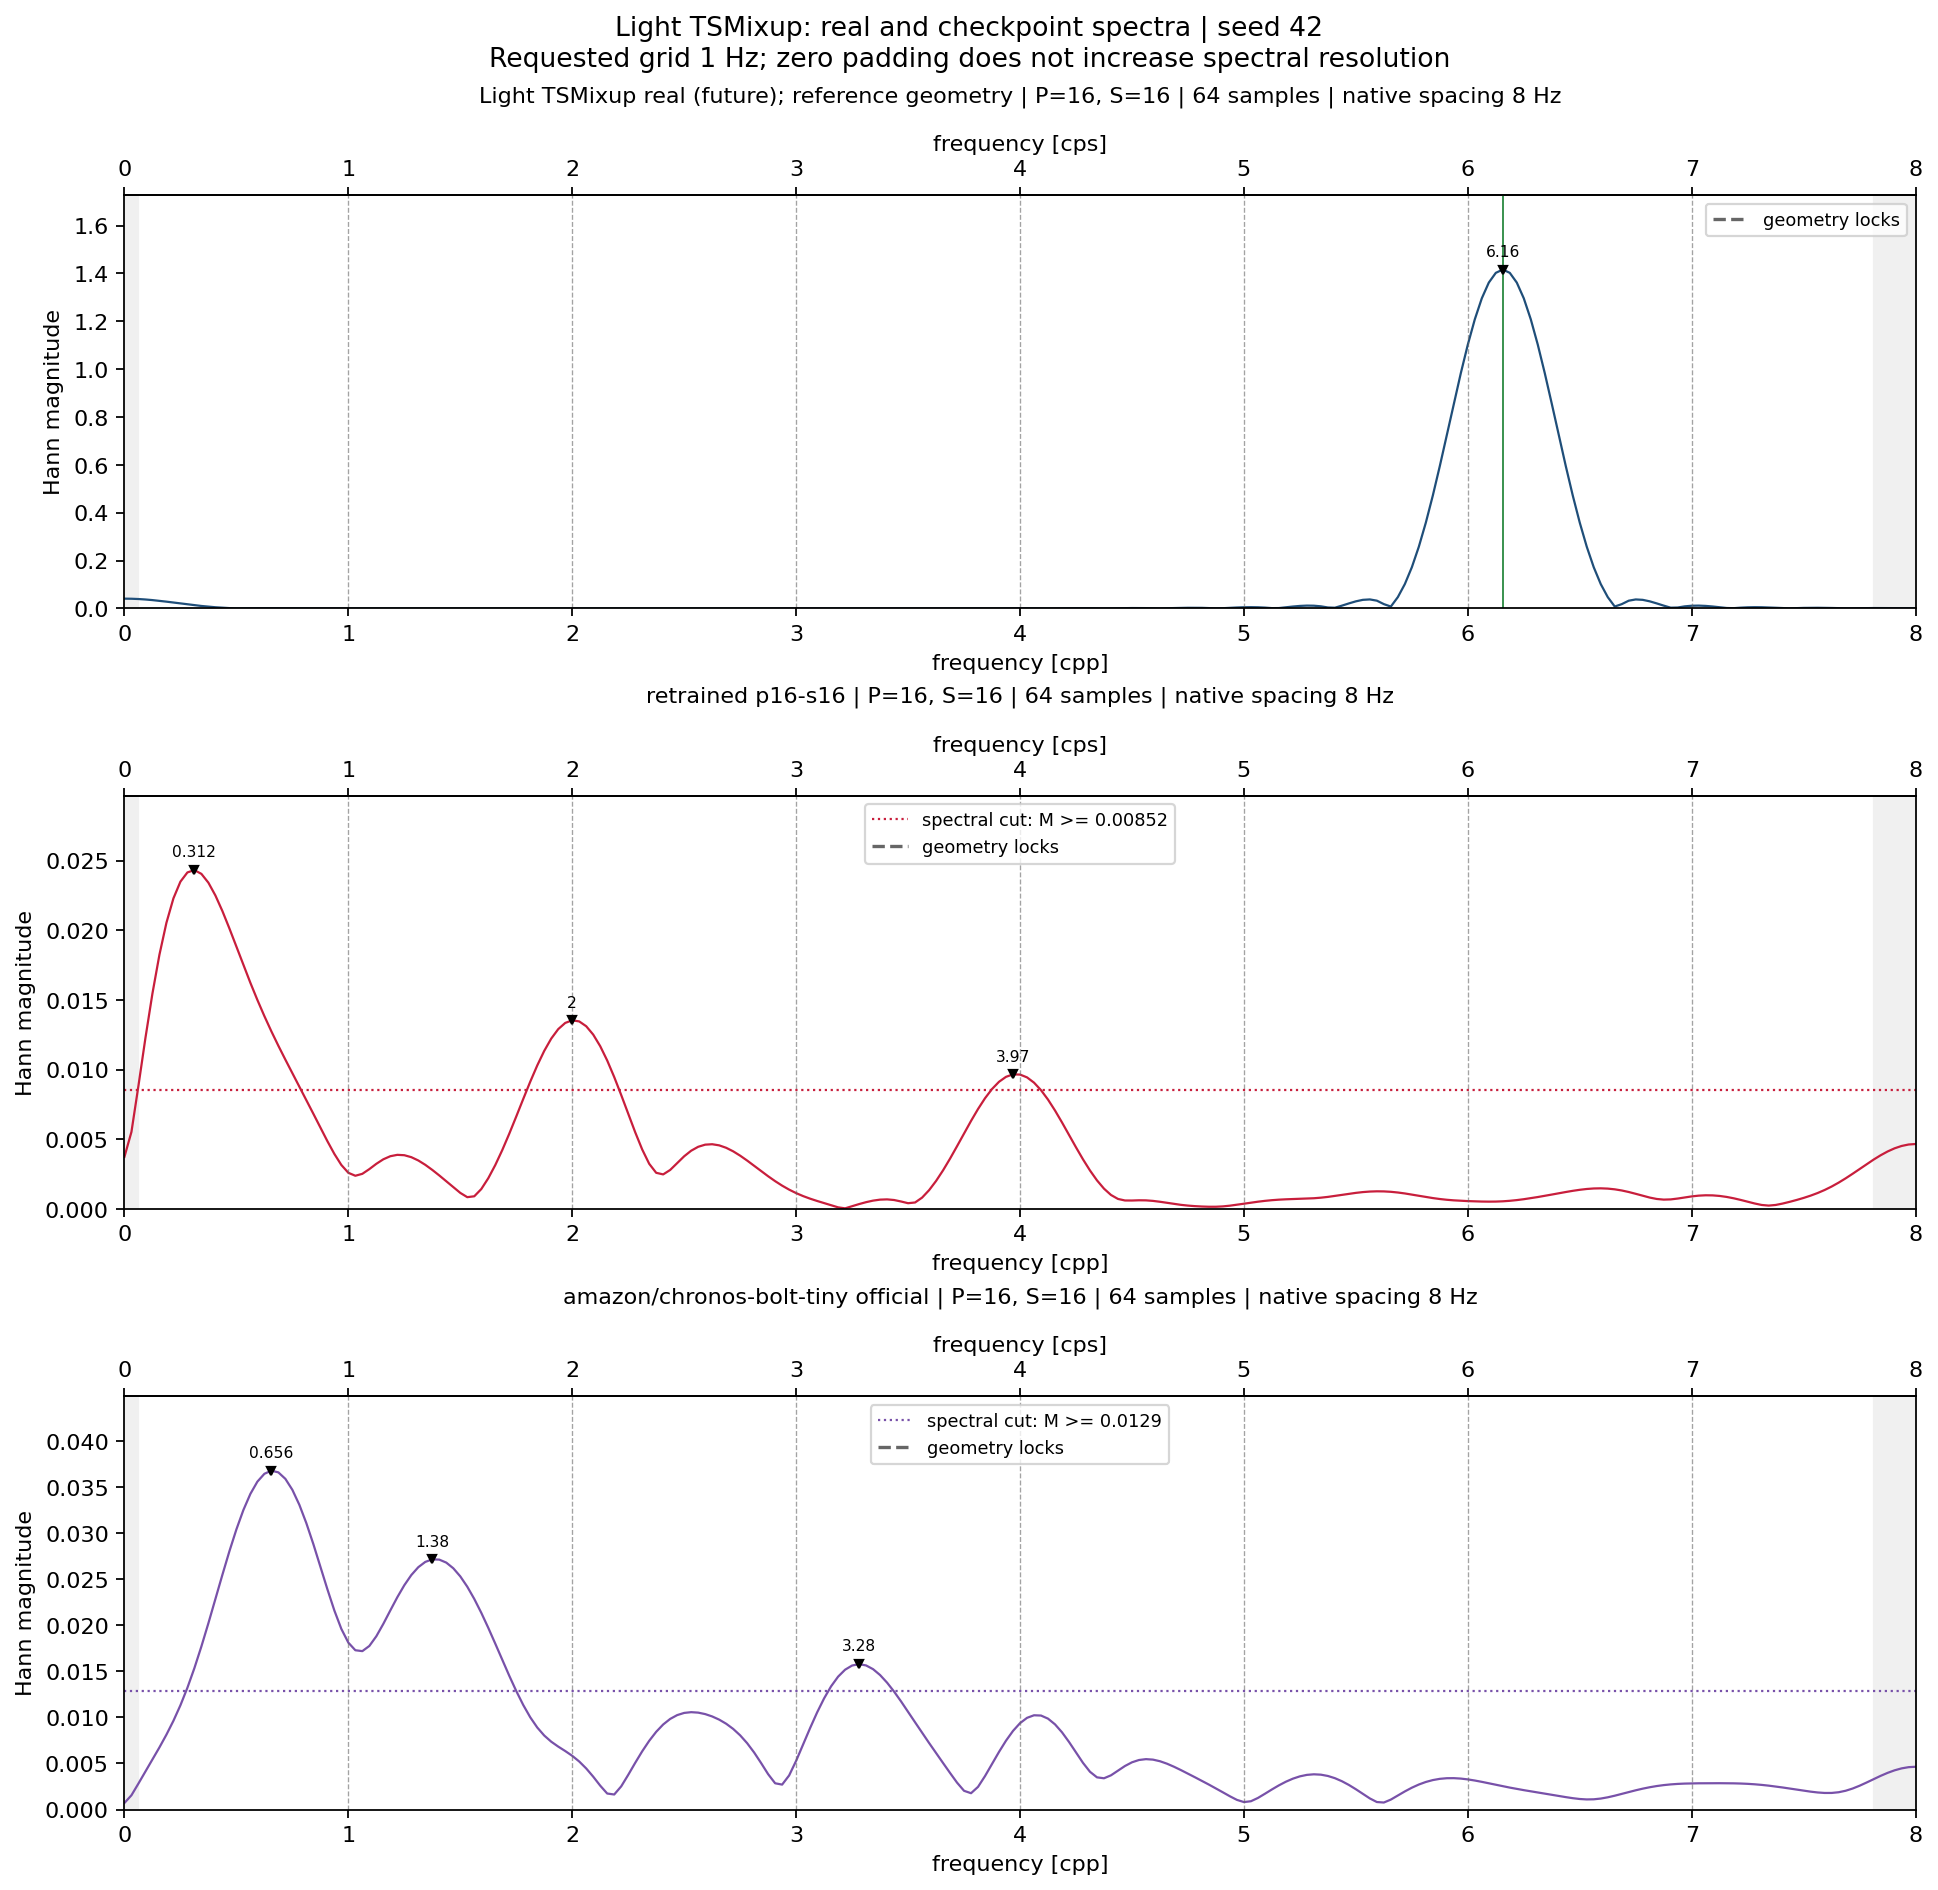
\includegraphics[width=\textwidth,height=0.80\textheight,keepaspectratio]{figures/FIG_G_tsmixup_p16-s16_seed42_spectra.png}
\caption{Spectra of the draw of \autoref{fig:decompTS}, read as \autoref{fig:decompKSspec}; the green vertical marks the frequency the generator drew. The two forecast panels have their own vertical scale, two orders of magnitude below that of the input.}
    \label{fig:decompTSspec}
\end{figure*}

\begin{figure*}[p]
    \centering
    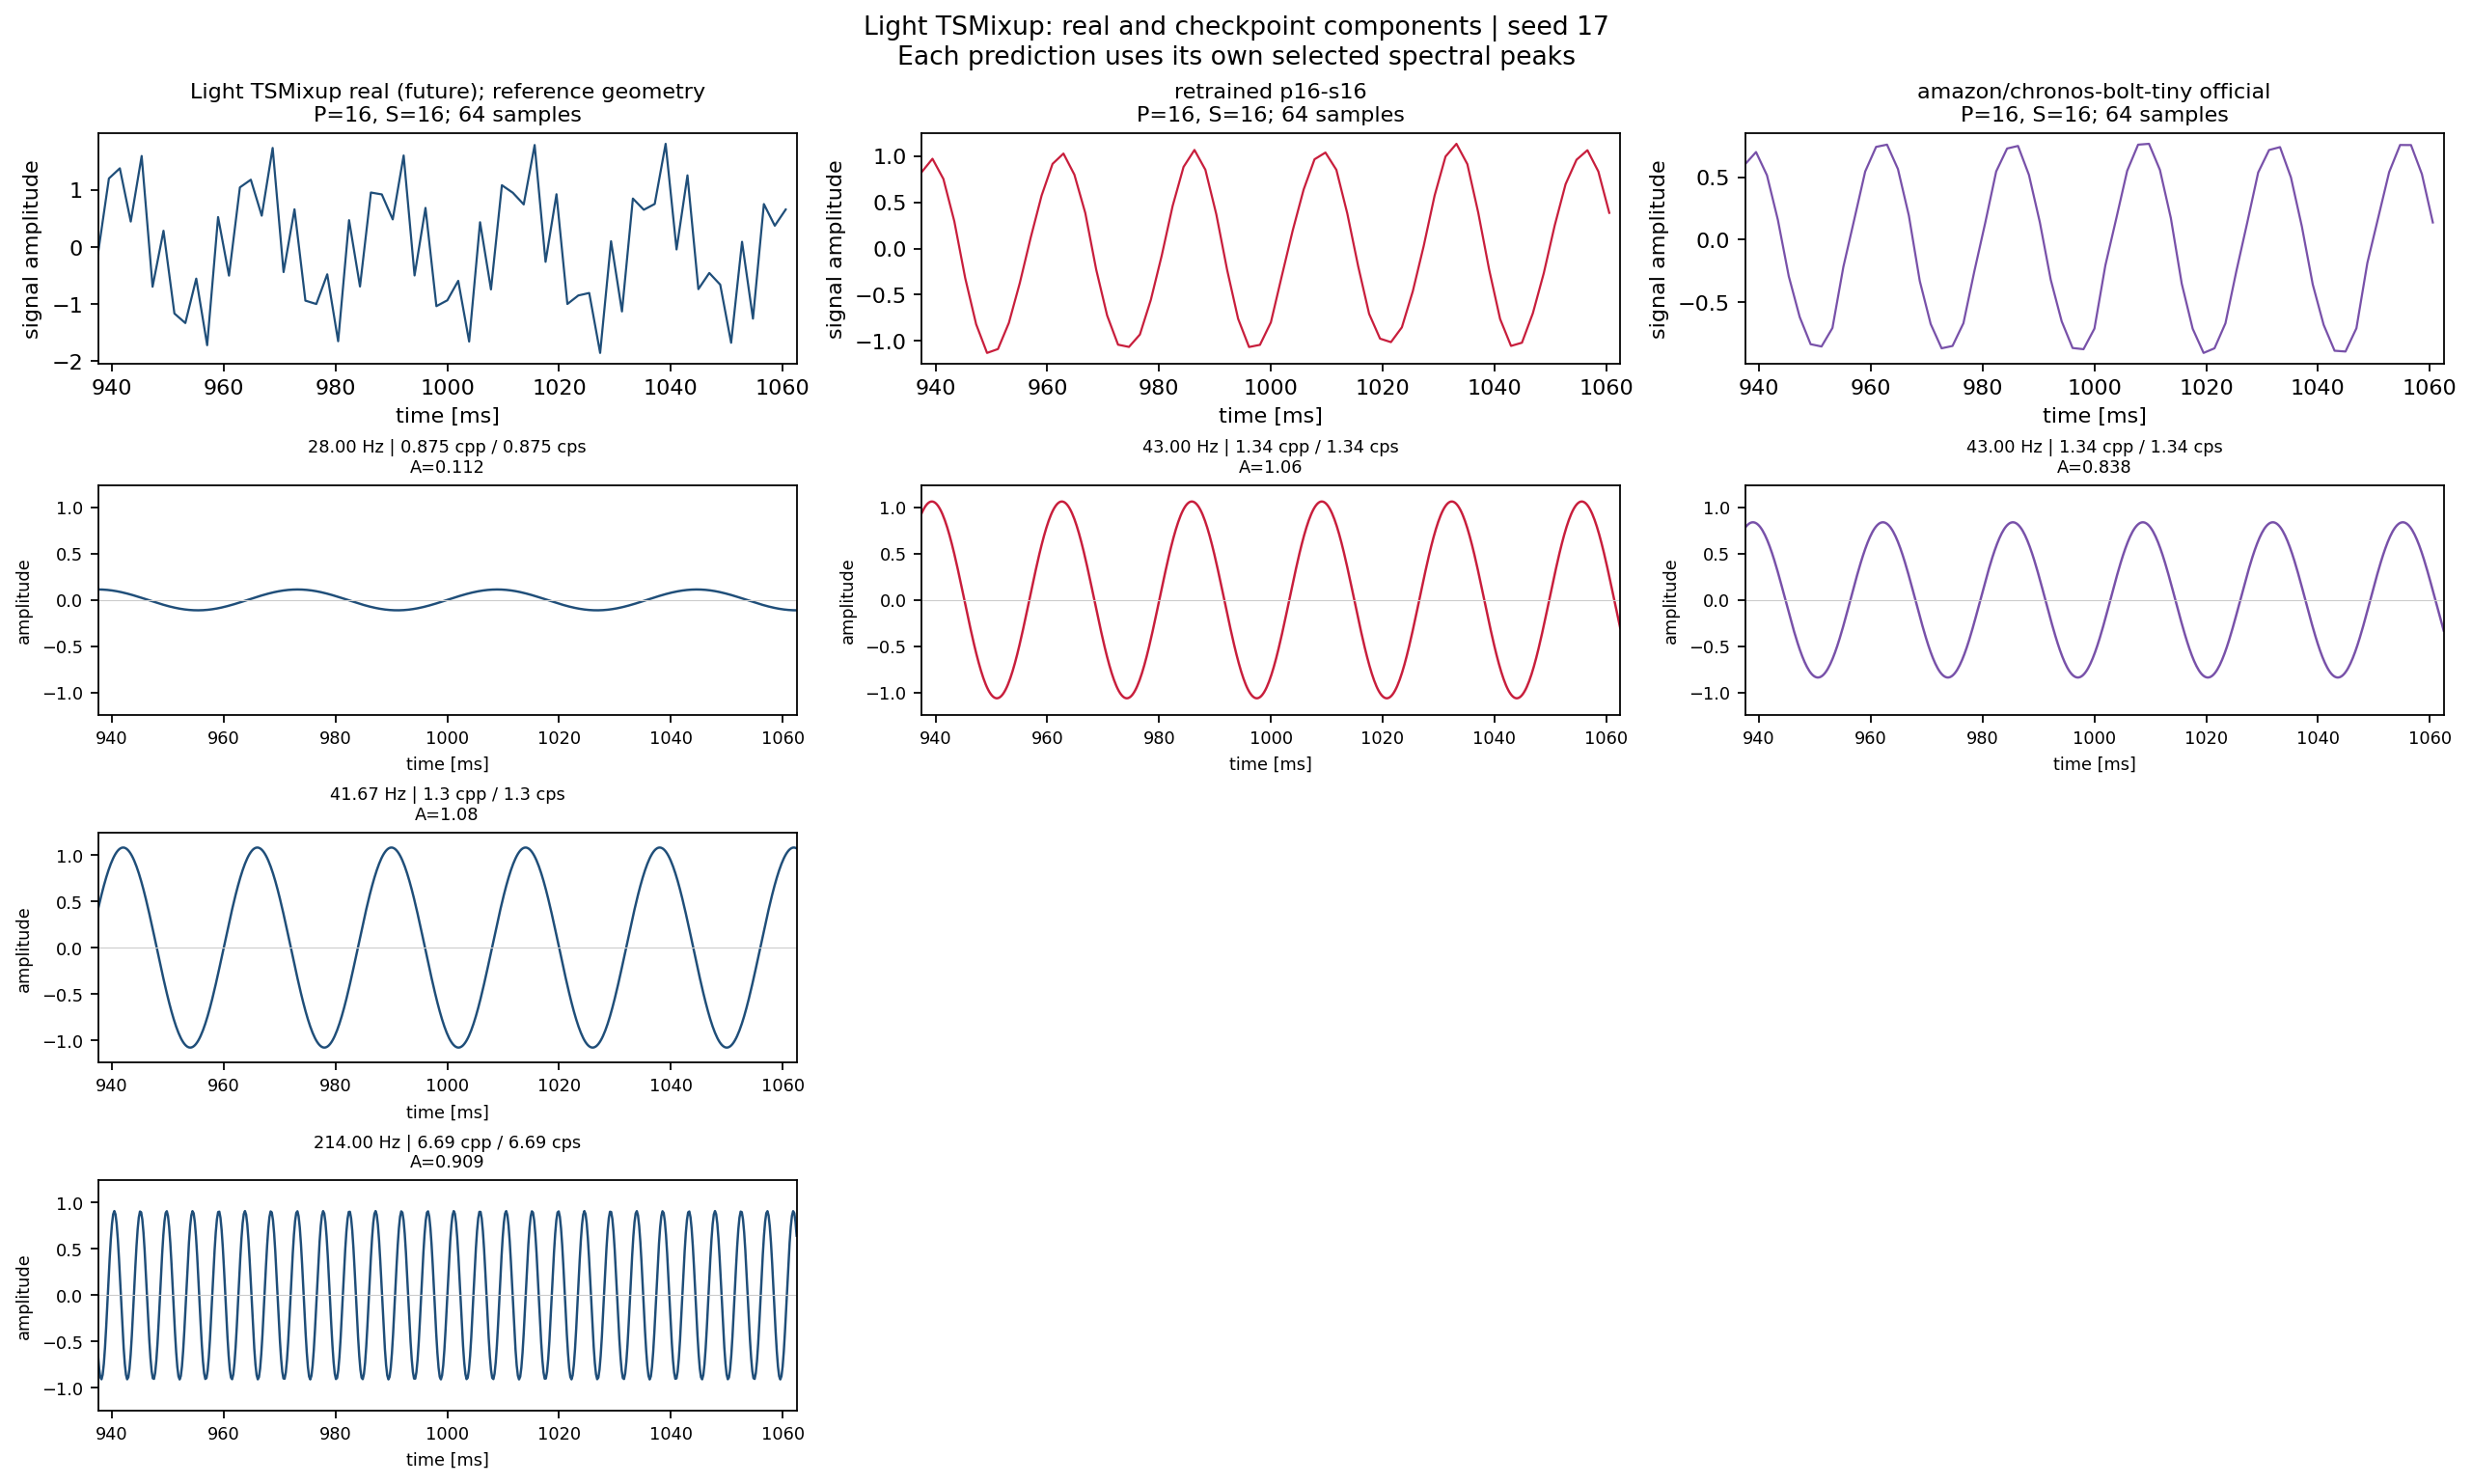
\includegraphics[width=\textwidth,height=0.70\textheight,keepaspectratio]{figures/FIG_G_tsmixup_p16-s16_seed17_components.png}
\caption{Light TSMixup draw with a low-frequency injected tone at $1.30$\,cpp in a background that also holds components at $0.88$ and $6.69$\,cpp, reference geometry $P=S=16$, components, read as \autoref{fig:decompKS}. Both checkpoints return the injected tone, at $1.34$\,cpp, and neither returns the $6.69$\,cpp component. Illustrative only: the aggregate is \autoref{tab:decomposition}.}
    \label{fig:decompTSlow}
\end{figure*}

\begin{figure*}[p]
    \centering
    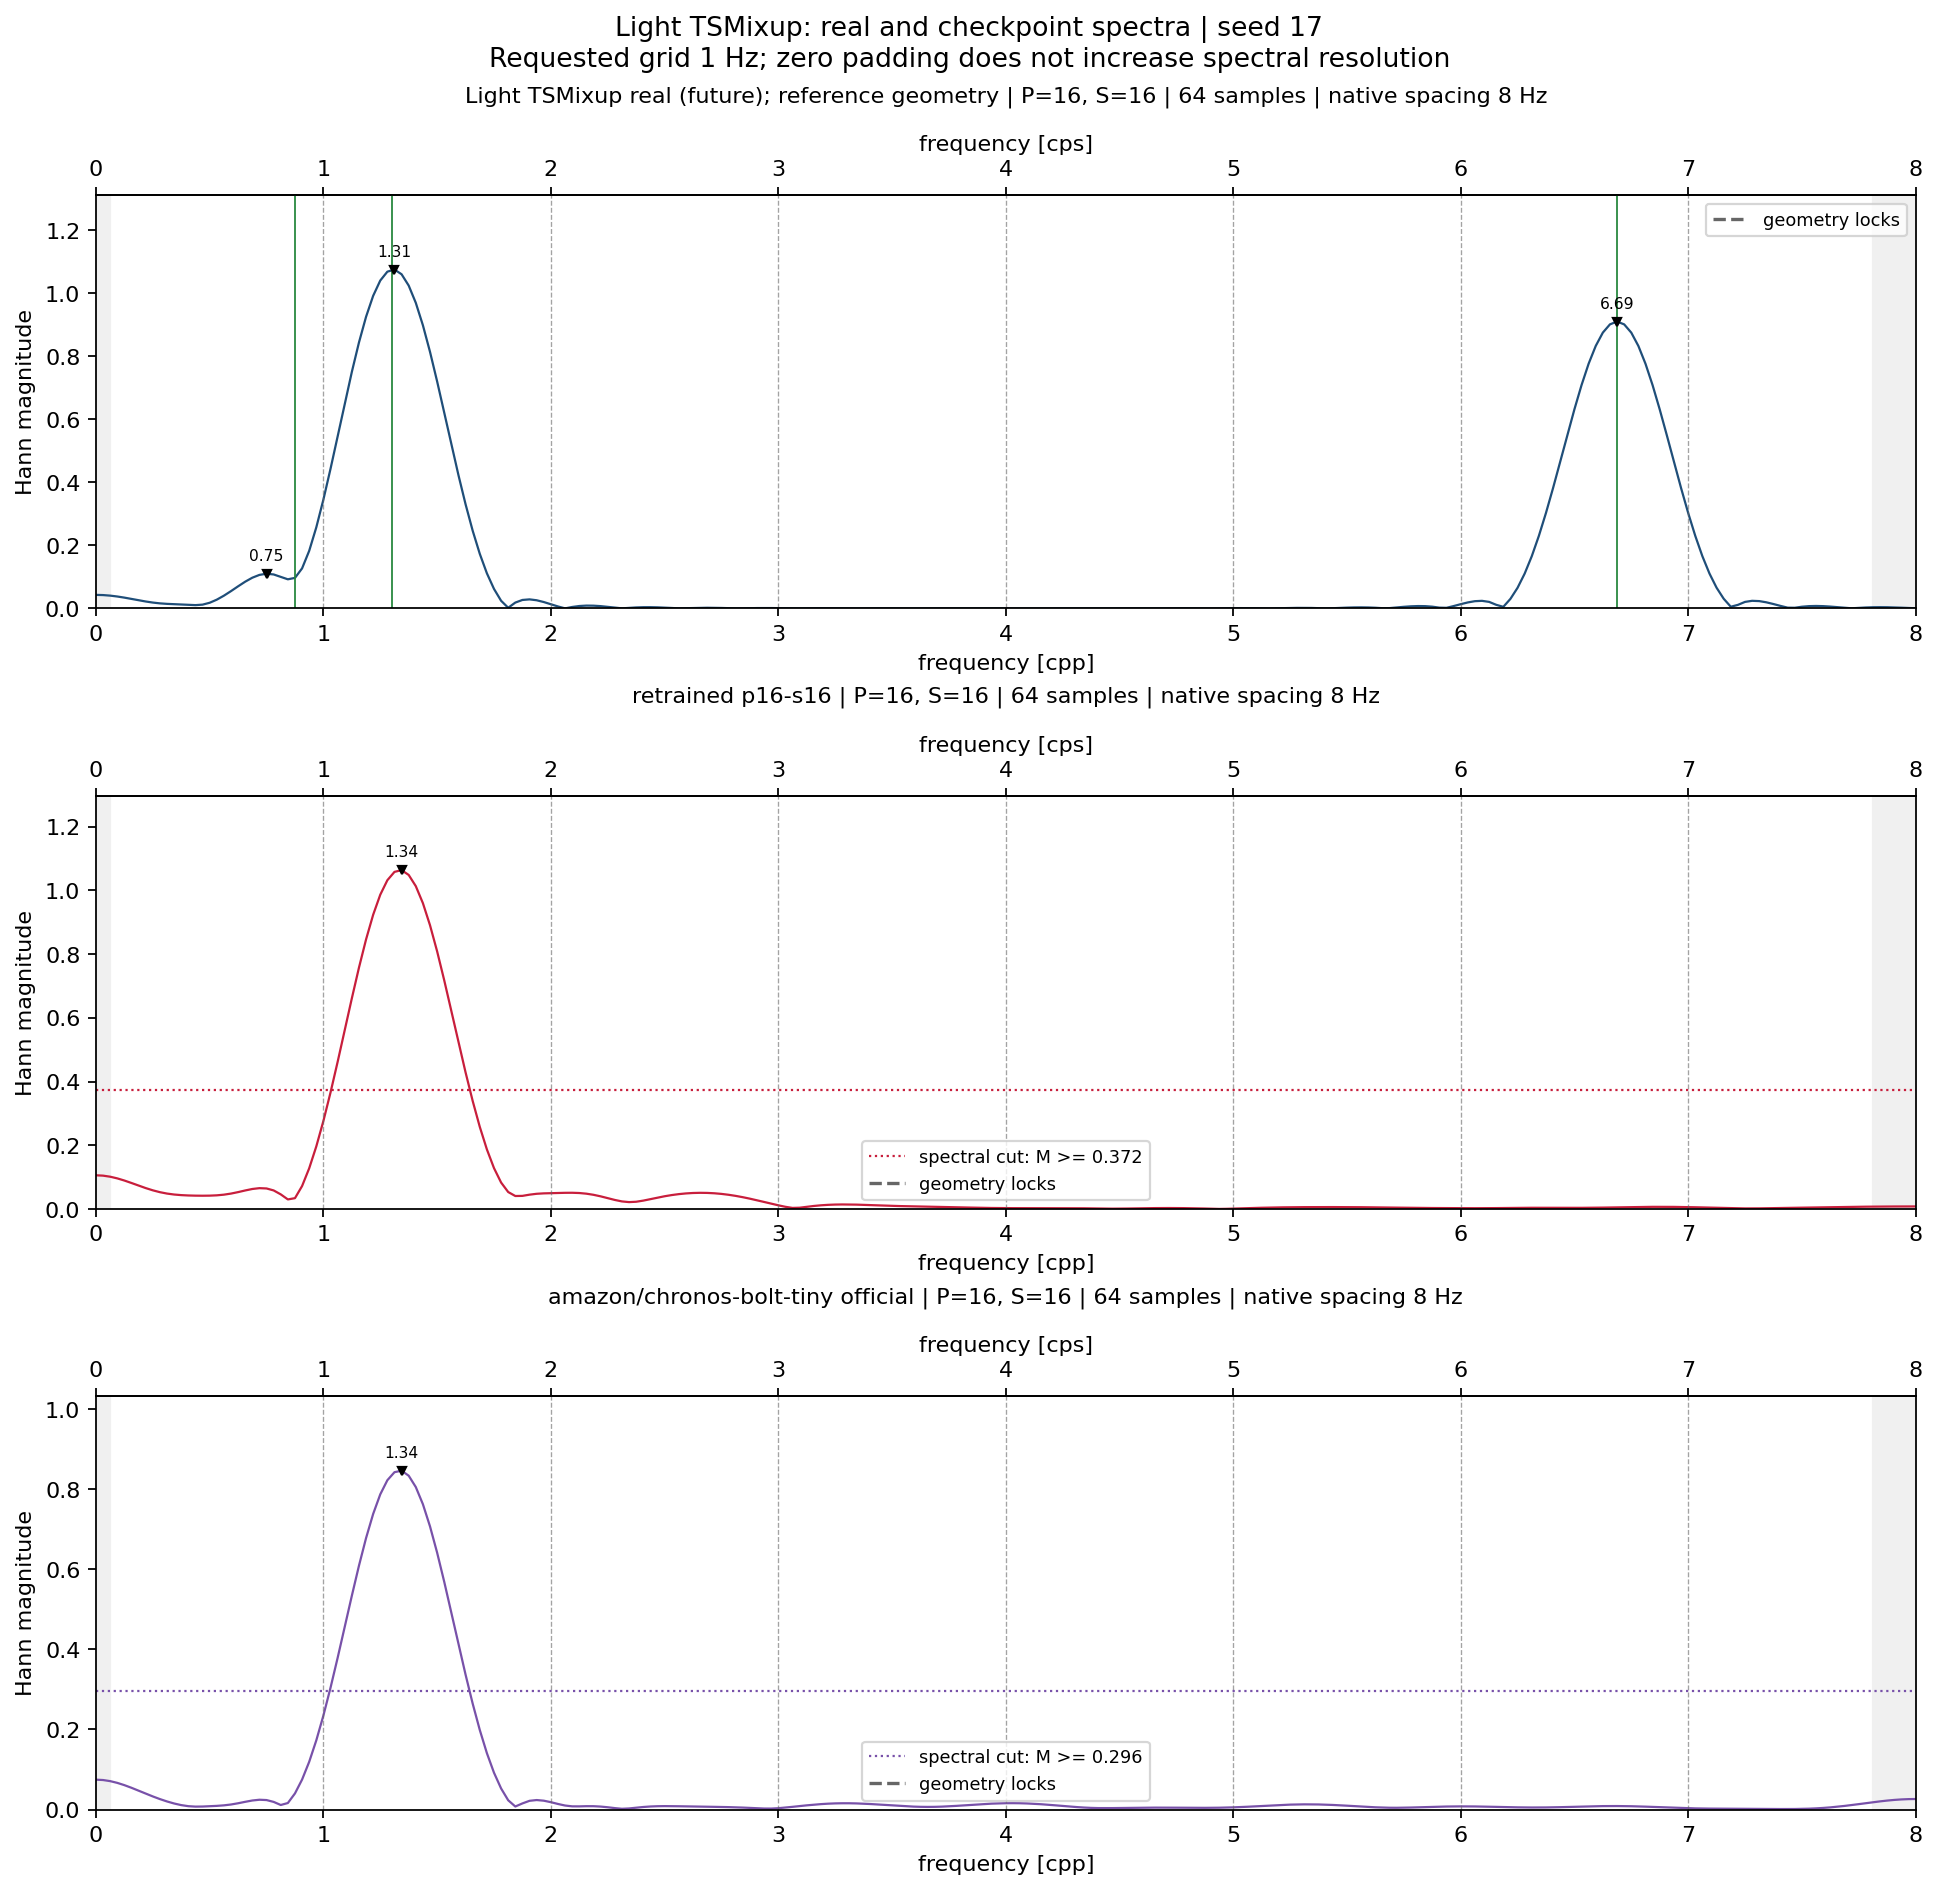
\includegraphics[width=\textwidth,height=0.80\textheight,keepaspectratio]{figures/FIG_G_tsmixup_p16-s16_seed17_spectra.png}
\caption{Spectra of the draw of \autoref{fig:decompTSlow}, read as \autoref{fig:decompKSspec}; green verticals mark the three frequencies the generator drew.}
    \label{fig:decompTSlowspec}
\end{figure*}

Read together, the three draws illustrate the behaviour that the recovery count quantifies: slow content tends to survive into the forecast and fast content tends to be lost, the published checkpoint returns more components than the retrained one, and the lines the retrained model returns away from the input often sit on its own candidate sites. This describes how the models behave on these signals and does not confirm any hypothesis, which is decided only by the paired analysis of \autoref{sec:bayesResults}.

\FloatBarrier
\subsection{The recovery count}

The single draws show what happens to one realisation; the count behind \autoref{tab:decomposition} asks how often an added component survives. For each generator one hundred backgrounds are drawn with the recipe above and reused unchanged for every checkpoint. Each geometry then receives one hundred paired trials: in the lock trial a tone is added at one of that geometry's candidate sites, the sites being cycled so that each is used about equally often, and since no geometry has a hundred sites in band, sites recur. In the control trial the same background receives a tone at a nearby frequency, placed below or above the site in equal proportion and more than $2$\,Hz from every candidate of that geometry. These controls serve only this count and differ from those of Model~A, which sit at a matched offset $f_k\pm\delta$ from each candidate (\autoref{sec:appBayes}). The tone has an amplitude of one and a half times the background standard deviation and the same phase in both trials of a pair, and the sum is not renormalised afterwards. The published checkpoint and the retrained $P=S=16$ share the same candidate sites and receive exactly the same signals.

Each forecast is decomposed as above, with up to eight candidate lines and the $35\%$ cut. A trial counts as recovered when any retained line lies within $\pm1$\,Hz of the added tone, bounds included. All one hundred trials remain in each denominator, and a forecast that cannot be produced stops the count rather than being dropped from it, so a geometry cannot improve its rate by failing on the difficult cases.

\autoref{tab:decomposition} in \autoref{sec:results} reports the outcome. The retrained models seldom return an added component, on average in about a quarter of the lock trials and in two per cent of the control trials. When a tone does reappear it is therefore mostly on a candidate site, while the same tone placed beside a site is almost always absorbed into a forecast dominated by its slowest content. The smallest patch retains the most, above half of the lock trials at $P=S=8$, and the widest patches the least, down to five or six per cent, with the same ordering for both generators. The published checkpoint returns added components more often both on and off the sites, $42$ and $16$ per cent on Light TSMixup backgrounds against $23$ and $1$ for the retrained $P=S=16$. Since the two share their geometry and receive the same signals, the difference is more plausibly related to training than to tokenisation, the retrained models following the published Chronos recipe under a reduced budget (\autoref{sec:appRetraining}).

Three limits bound what the count can say, the first being that it measures presence in the output and not attribution, since the background may already carry energy near the added frequency and nothing is subtracted for it. The single draws add a sharper form of the same caveat. The retrained forecasts carry lines of their own on the candidate sites even where the input holds nothing there, at $4$\,cpp in \autoref{fig:decompKS} and at $2$ and $4$\,cpp in \autoref{fig:decompTS}, and such a line is credited as a recovery whenever the tone of a lock trial sits on it. The count therefore includes a background-only arm, the same draws forecast without the added tone and scored at the lock and control frequencies, and credits a net recovery only when that forecast has no line within one hertz of the tone. With no tone added, the retrained forecasts already carry a line within one hertz of the lock frequency in $11\%$ of the Light TSMixup backgrounds and $6\%$ of the KernelSynth ones on average, and beside a control in about one per cent. Discounting those lines lowers the lock rate from $25.9$ to $16.1\%$ on Light TSMixup and from $24.9$ to $19.2\%$ on KernelSynth, while the control rate moves from about two per cent to $1.8$ and $1.7\%$, so most of the asymmetry survives (the Net column of \autoref{tab:decomposition}). The reference geometry is the exception on Light TSMixup, where the model's own lines explain most of the rate, $19\%$ of the backgrounds carrying one against $23\%$ of the trials recovered, leaving $6\%$ net; the published checkpoint keeps $33\%$ net on both generators. The one-hertz tolerance is finer than the native spacing, so a recovered line is one located near the tone, not one resolved from its neighbours. And the count carries no interval, so it describes the geometries at a high level and is not a statistical test.



\flushfloatpages
\appendixsection{The Photovoltaic Series}{sec:appSolar}
This appendix describes how the photovoltaic series is prepared, forecast and scored for \autoref{sec:results}. It covers three pieces of work: an inspection of the record day by day, a single forecast examined in detail, and a benchmark over many windows spread across the year. All three are descriptive, and the series is the application domain of the study and is used for high-level insight only.

\subsection{The record}

The series is the module power of the SolarTech Lab plant\autocite{levaPhotovoltaicPowerWeather2020}, recorded once per minute over the whole of 2017 and timestamped in Central European Time, $525{,}601$ timestamps in total. Only $198{,}730$ of them, $37.8\%$, carry a valid reading. Power is absent outside daylight by construction, because the plant produces nothing and the logger records nothing; during the day readings are also lost whenever the logger misses a minute. Twenty readings above $1$\,kW, with a maximum near $60$\,kW, are physically impossible for this module and are treated as missing rather than as data.

Each day is inspected by locating its longest run of consecutive valid readings, which is the longest stretch that could be handed to a model without any filling. The longest run in the whole year is $880$ minutes, on 5 July, and only $64$ of the $365$ days reach the $544$ consecutive readings used by the synthetic windows. \autoref{fig:solarDays} shows two of the longest runs: on the clear day the power traces a smooth arc that peaks near $200$\,W, whereas on the cloudy one the midday readings scatter well away from that arc. \autoref{fig:solarOverlay} superimposes four days of different character: clear summer days follow a smooth arc, a winter day produces less power over a shorter interval, and a cloudy day departs from the arc in rapid drops and peaks that last a few minutes each. Those departures come from the weather and not from the plant, so they are part of what a forecaster is asked to predict and cannot learn from the context.

\begin{figure}[!htbp]
    \centering
    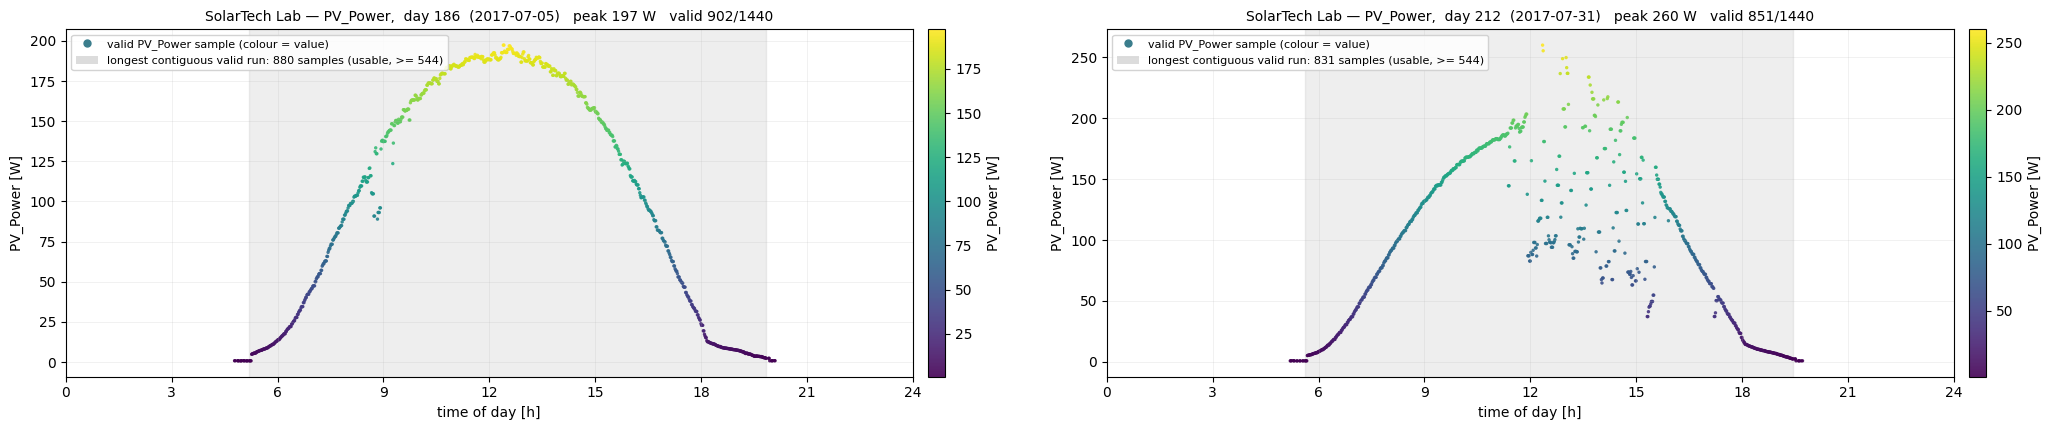
\includegraphics[width=\textwidth]{figures/SOLAR_days_186_212.png}
\caption{Module power over two recorded days, 5 July (left) and 31 July 2017 (right), one point per valid minute coloured by its value. The grey band marks the longest run of consecutive valid readings in each day. The first day is clear and follows the expected arc; on the second, the scattered readings between noon and mid-afternoon are drops and peaks caused by passing clouds and changing weather.}
    \label{fig:solarDays}
\end{figure}

\begin{figure}[!htbp]
    \centering
    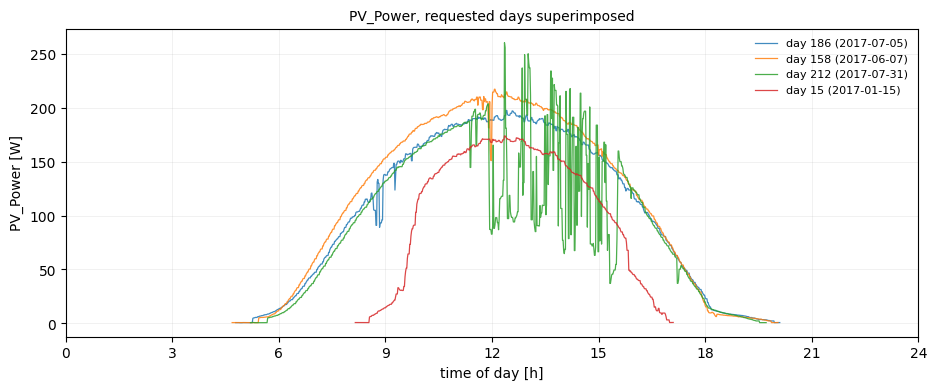
\includegraphics[width=0.9\textwidth]{figures/SOLAR_days_overlay.png}
\caption{Module power on four recorded days, superimposed by time of day: two clear summer days (5 July and 7 June), a summer day with passing clouds (31 July) and a winter day (15 January). Gaps in a curve are minutes without a valid reading.}
    \label{fig:solarOverlay}
\end{figure}

\subsection{From a record with gaps to a model input}

A context is the $2048$ minutes that precede the moment the forecast is issued, taken as they fall in the record, so it always crosses at least one night and reaches into the previous day. Because the model cannot be given an absent value, every missing minute of the context is resolved by one of three rules. A minute with the sun below the horizon, computed from the site coordinates and the date, is set to zero, since that is the power the plant actually produces then. A daytime gap of at most $15$ minutes is bridged by a straight line between the valid readings on either side of it. Any remaining daytime gap is also set to zero, and is the only filling that may differ from what the plant did. In the benchmark the bridging uses only readings that precede the forecast time, so no information from the horizon enters the context.

The horizon is treated differently, because it is what the forecast is scored against. A horizon minute is kept if it was measured, or if it falls at night, where its value is known to be zero. A missing daytime minute is excluded from the score rather than filled, since its true value is not known.

\subsection{Reading minutes in cycles per patch}

The tokeniser sees a sequence of samples and has no notion of seconds, so the series is given to the model as it is, without resampling. A component whose period is $T$ samples completes $P/T$ cycles in a patch and $S/T$ in a stride, whatever the sampling rate, and the candidate condition of \autoref{sec:tokenisation}, a whole number of cycles per patch or per stride, reads the same on this series as on the synthetic signals. At one sample per minute and $P=S=16$, the first candidate sites are periods of $16$, $8$ and $16/3$ minutes. Variations of that speed exist in the record only as the short weather transients described above; the dominant content of a window is the daily cycle, whose period is some hundred times longer.

\subsection{One forecast in detail}

A single forecast is first examined in detail, issued at 13:00 on 5 July 2017, the day with the longest valid run, and repeated for the published checkpoint and for every retrained geometry on the same context. It is complemented by the winter forecast of \autoref{fig:solarForecast19} in the benchmark below, and is a summer day of a different kind. The context starts at 02:52 on the previous day; $1377$ of its $2048$ minutes are measured, $634$ night-time minutes are set to zero, $37$ minutes of short daylight gaps are bridged, and all $64$ horizon minutes are measured.

\begin{figure}[!htbp]
    \centering
    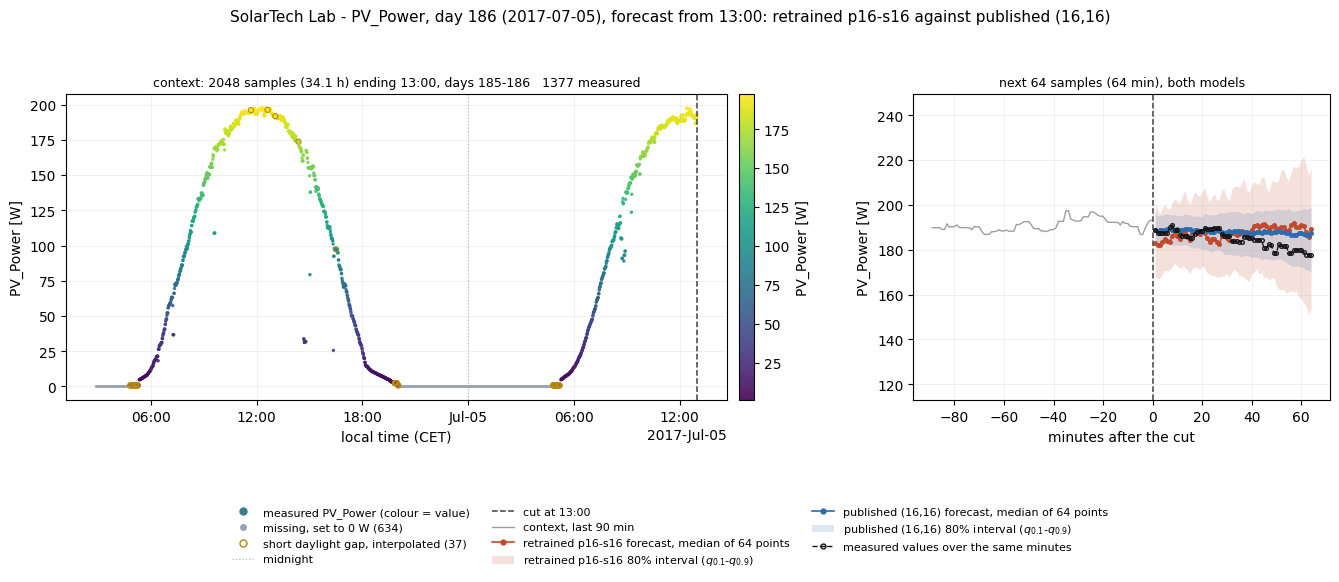
\includegraphics[width=\textwidth]{figures/SOLAR_day186_1300_p16-s16_both.png}
\caption{Forecast issued at 13:00 on 5 July 2017 by the retrained $P=S=16$ geometry and by the published checkpoint. Left, the full context with its measured, zero-filled and interpolated minutes marked; right, the last $90$ minutes of context and the $64$ forecast minutes, with each model's median and $80\%$ interval against the measured values.}
    \label{fig:solar186both}
\end{figure}

\autoref{fig:solar186both} and \autoref{fig:solar186err} show the reference geometry against the published checkpoint. Both continue the midday level near $188$\,W while the measured power starts to decline after about half an hour, and both intervals contain all $64$ measured minutes. The error is small in either case, $5.3$\,W for the retrained model and $3.8$\,W for the published one, and it grows along the horizon as the two medians stay flat above a falling measurement.

\begin{figure}[!htbp]
    \centering
    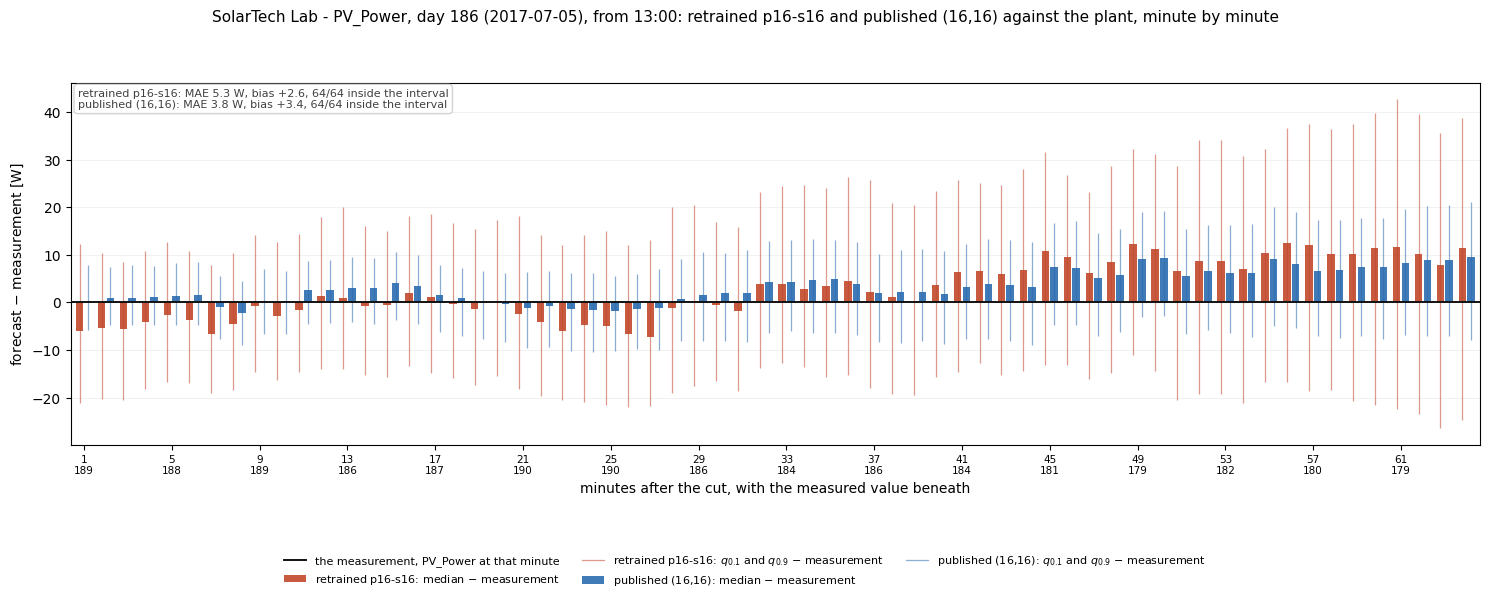
\includegraphics[width=\textwidth]{figures/SOLAR_day186_1300_p16-s16_error.png}
\caption{The same forecast as \autoref{fig:solar186both}, drawn as the difference between forecast and measurement minute by minute: bars for the medians, thin lines for the $10\%$ and $90\%$ quantiles, with the measured value printed beneath each labelled minute.}
    \label{fig:solar186err}
\end{figure}

Across the fifteen geometries the same cut gives errors between $5.3$ and $15.9$\,W. \autoref{fig:solar186patch} groups their medians by patch size, and the forecasts spread over about $40$\,W at $P=24$ and $P=32$, some rising and some falling, while the measurement moves by ten watts, and within a patch size the order of the curves does not follow the stride. One cut on one day cannot separate the geometry from the particular window, which is why the benchmark below repeats the comparison over many windows.

\begin{figure}[!htbp]
    \centering
    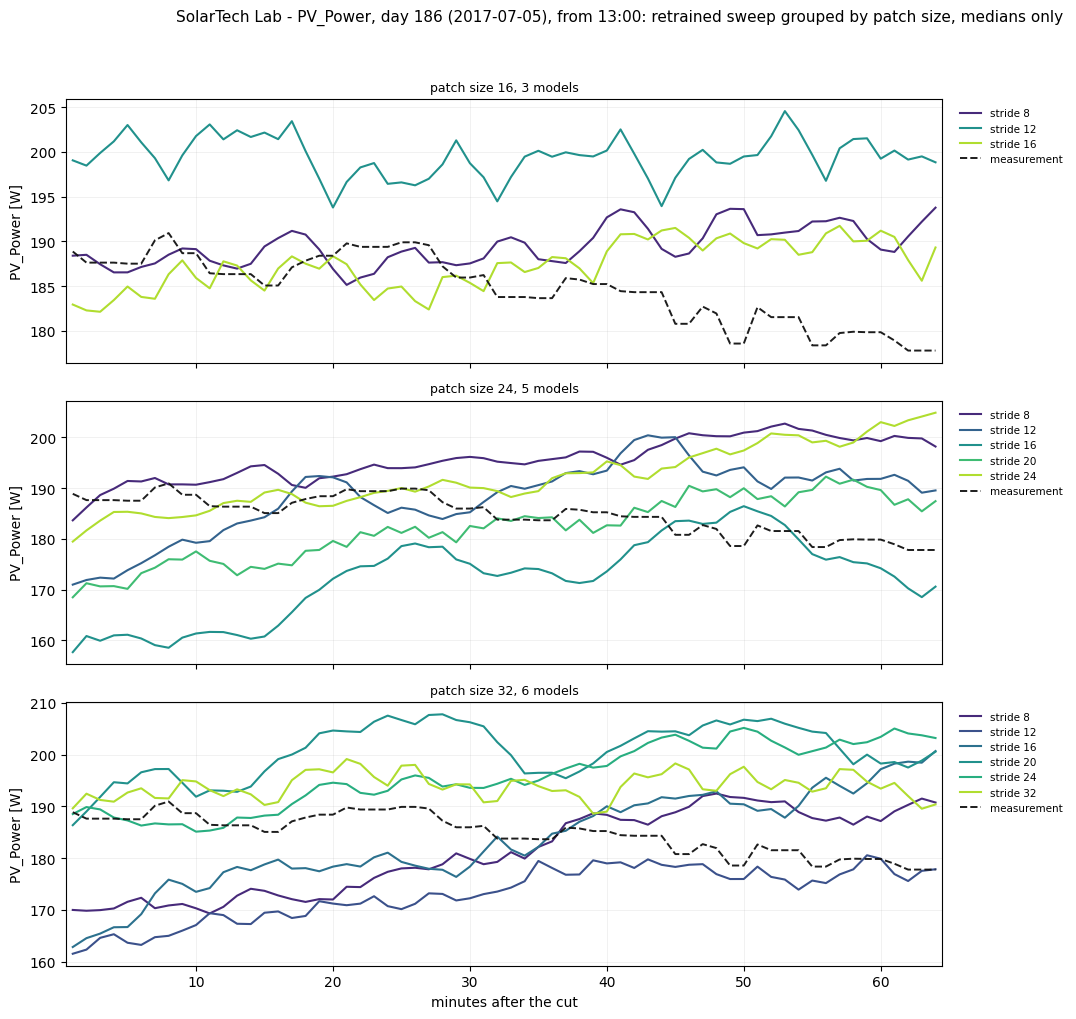
\includegraphics[width=0.8\textwidth]{figures/SOLAR_day186_1300_bypatch.png}
\caption{Median forecasts of the retrained geometries for the cut of \autoref{fig:solar186both}, one panel per patch size and one colour per stride, against the measured values (dashed). Intervals are omitted so that the curves remain readable.}
    \label{fig:solar186patch}
\end{figure}

\subsection{The benchmark over the year}

The benchmark draws $150$ windows of $2048+64$ minutes each, chosen at random over the whole year under the constraint that no two windows share a minute, from a fixed seed so that the selection can be reproduced. Each draw removes every start that would overlap it, so the selection is a seeded random packing rather than a uniform sample of all disjoint sets, and it is not balanced by hour of day. Every model forecasts exactly the same windows from exactly the same contexts, and every model is scored on the same minutes. Each window is assigned to one of three regimes by the solar elevation at the time its forecast is issued: night at or below $0^\circ$, the transition around sunrise and sunset up to $10^\circ$, and day above it. All its scored minutes are counted in that regime, so that the near-zero night-time error does not dilute the daytime one. Of the $9{,}187$ minutes scored per model, $4{,}777$ fall in windows issued at night, $822$ in the transition and $3{,}588$ in daylight.

The point forecast is the median of the nine quantiles each model returns. For each model the mean absolute error, the mean error or bias, the variance of the error and the root mean square error are computed over all scored minutes, and the weighted quantile loss is computed over all nine quantiles to judge the forecast distribution rather than its median alone. Each model is also compared with two references, the published checkpoint and the retrained $P=S=16$, through the paired difference in mean absolute error. Its $95\%$ interval runs from the $2.5$th to the $97.5$th percentile of a bootstrap that resamples whole weeks, $51$ of them, $2000$ times, so that windows falling in the same week are not treated as independent. An interval that contains zero means the two models cannot be told apart on this series; it does not mean that they are equal.

\autoref{tab:solarPrediction} reports the error of the median forecast, overall and by regime of the daily cycle, with the comparison with the retrained baseline, and \autoref{tab:solarVsOfficial} reports the quantile loss and the comparison with the published checkpoint. The error is concentrated in daylight, where the forecast has to follow a changing level, and it grows through the transitions around sunrise and sunset into the day itself, whereas at night almost every model correctly continues a series held at zero. Among the retrained models none improves on the $P=S=16$ baseline: p8-s8, p16-s8, p24-s12, p24-s24 and p32-s32 cannot be told apart from it, the others are worse by roughly two to five watts, apart from p32-s20, which has the largest error of all, and neither overlap nor patch size orders them. Every retrained geometry is worse than the published model, by between $1.9$ and $7.6$\,W apart from p32-s20, and the quantile loss orders the models almost exactly as the mean absolute error does.

\begin{table}[!tbp]
    \centering
    \small
    \renewcommand{\arraystretch}{1.1}
    \begin{tabular}{@{}ccccc@{}}
        \toprule
        & & & \multicolumn{2}{c}{\textbf{$\Delta$MAE vs published}} \\
        \cmidrule(l){4-5}
        \textbf{$P$} & \textbf{$S$} & \textbf{WQL} & \textbf{Estimate} & \textbf{Interval} \\
        \midrule
        $16$ & $16^{\dagger}$ & $0.152$ & --- & --- \\
        \midrule
        $8$ & $8$ & $0.210$ & $+3.16$ & $[1.97,\,4.37]$ \\
        \midrule
        $16$ & $8$ & $0.191$ & $+1.91$ & $[1.08,\,2.79]$ \\
        $16$ & $12$ & $0.291$ & $+6.65$ & $[4.96,\,8.43]$ \\
        $16$ & $16$ & $0.200$ & $+2.52$ & $[1.40,\,3.63]$ \\
        \midrule
        $24$ & $8$ & $0.247$ & $+5.08$ & $[3.63,\,6.59]$ \\
        $24$ & $12$ & $0.206$ & $+3.16$ & $[2.18,\,4.23]$ \\
        $24$ & $16$ & $0.271$ & $+6.44$ & $[4.55,\,8.43]$ \\
        $24$ & $20$ & $0.300$ & $+7.59$ & $[5.72,\,9.50]$ \\
        $24$ & $24$ & $0.212$ & $+3.29$ & $[1.85,\,4.65]$ \\
        \midrule
        $32$ & $8$ & $0.275$ & $+6.37$ & $[4.89,\,7.79]$ \\
        $32$ & $12$ & $0.242$ & $+4.72$ & $[3.23,\,6.21]$ \\
        $32$ & $16$ & $0.251$ & $+5.39$ & $[3.93,\,6.90]$ \\
        $32$ & $20$ & $0.638$ & $+24.59$ & $[19.10,\,30.00]$ \\
        $32$ & $24$ & $0.248$ & $+5.29$ & $[3.79,\,6.90]$ \\
        $32$ & $32$ & $0.198$ & $+2.61$ & $[1.71,\,3.53]$ \\
        \bottomrule
    \end{tabular}
\caption{The probabilistic side of the benchmark and the comparison with the published checkpoint. WQL is the weighted quantile loss averaged over the nine forecast quantiles, lower being better; the last two columns give the paired difference in MAE, in watts, from the published checkpoint (row $\dagger$), with the same week-resampling bootstrap interval as \autoref{tab:solarPrediction}.}
    \label{tab:solarVsOfficial}
\end{table}


\begin{figure}[!htbp]
    \centering
    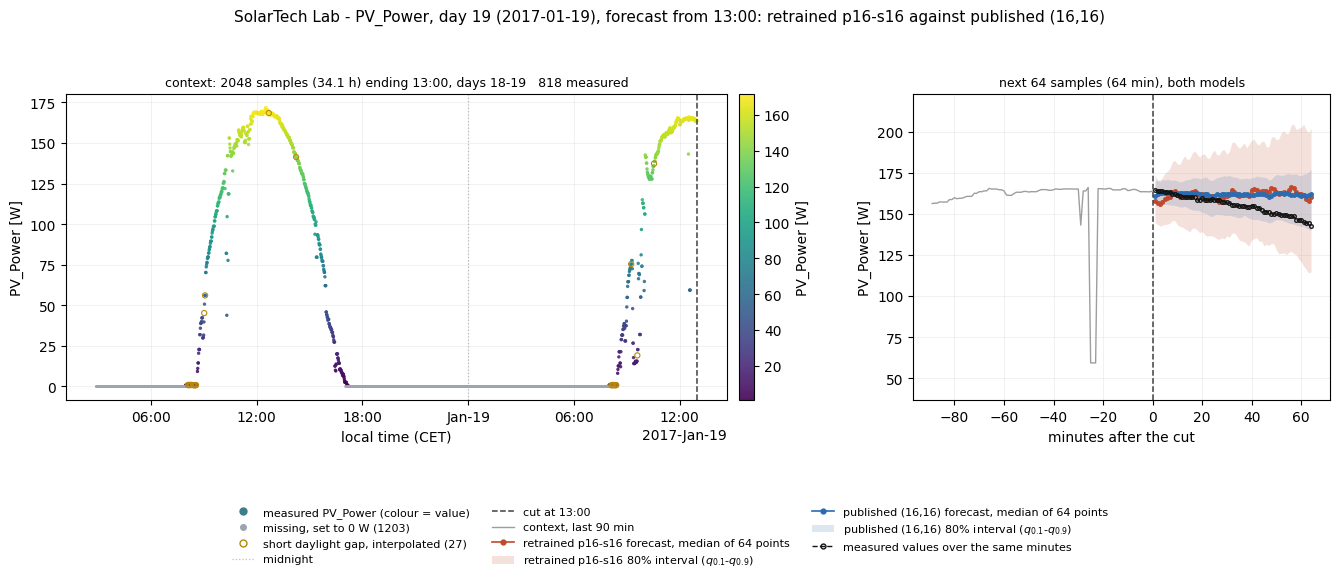
\includegraphics[width=\textwidth]{figures/SOLAR_day019_1300_p16-s16_both.png}
\caption{Forecast issued at 13:00 on 19 January 2017 by the retrained $P=S=16$ geometry and by the published checkpoint. Left, the $2048$-minute context, which spans the previous day and night: $818$ minutes are measured, $1203$ missing night-time minutes are set to zero and $27$ minutes of short daylight gaps are interpolated. Right, the last $90$ minutes of context and the $64$ forecast minutes, with each model's median and $80\%$ interval against the measured values.}
    \label{fig:solarForecast19}
\end{figure}

The forecast of \autoref{fig:solarForecast19}, issued on a winter afternoon at the reference geometry, illustrates that behaviour on one window. Both checkpoints prolong the level of the last hour while the measured power begins its afternoon decline, so the error grows along the horizon, and only the wider interval of the retrained model keeps the measurement within its bounds until the end.

\begin{figure}[!htbp]
    \centering
    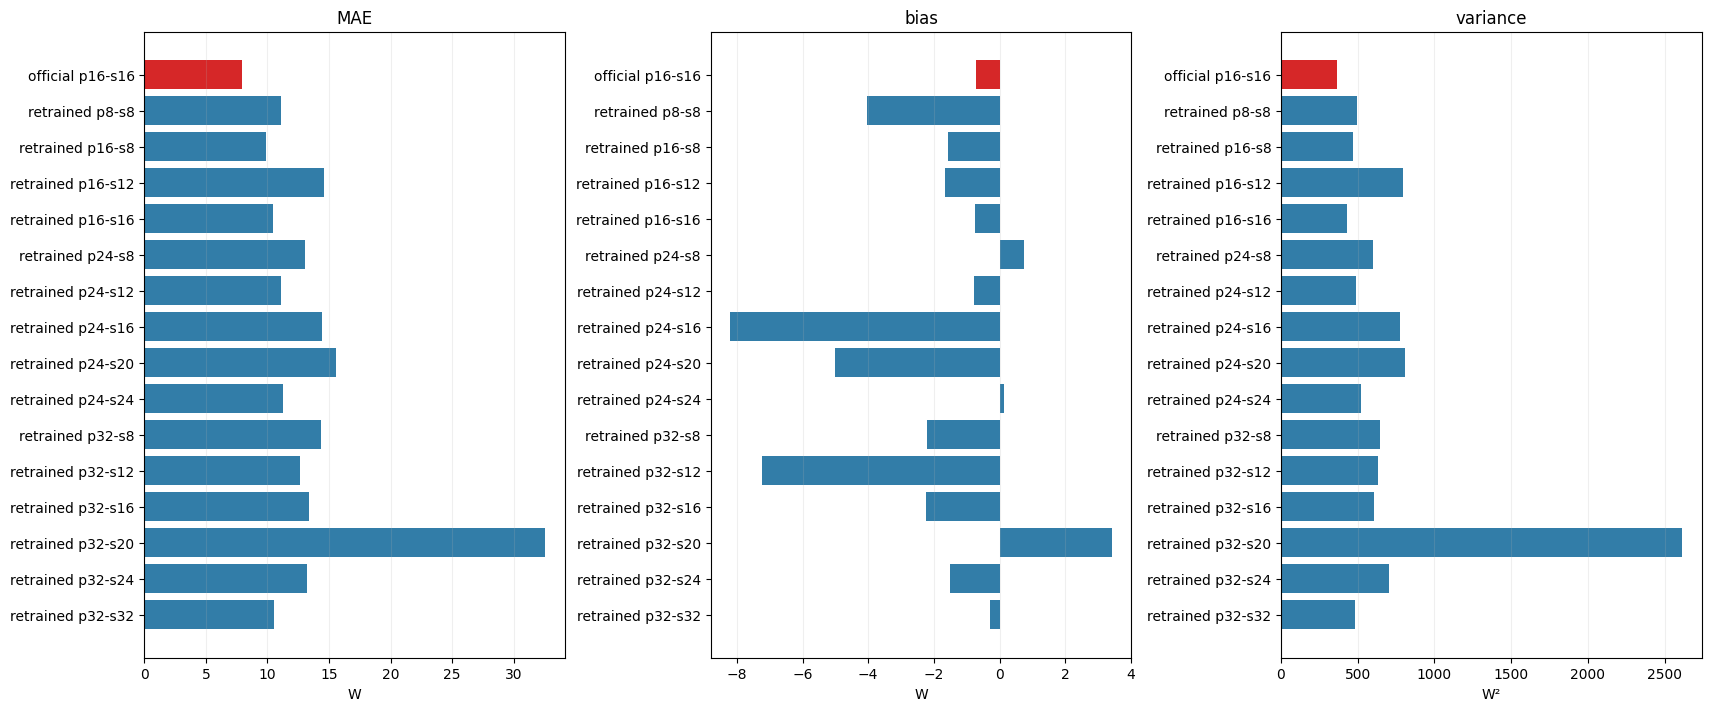
\includegraphics[width=\textwidth]{figures/SOLAR_benchmark_summary.png}
\caption{Mean absolute error, bias and error variance of the median forecast over the $150$ windows, for the published checkpoint (red) and the fifteen retrained geometries (blue).}
    \label{fig:solarSummary}
\end{figure}

\autoref{fig:solarSummary} draws the three measures side by side. The published checkpoint has the lowest mean absolute error and error variance and a bias close to zero. The retrained geometries form a band a few watts above it and mostly carry a negative bias, largest for p24-s16 and p32-s12, so they tend to under-forecast. The p32-s20 geometry has the largest mean absolute error of all.

\subsection{The dominant frequency of the context}

To place each window in the units of \autoref{sec:tokenisation}, the strongest non-constant component of its context is located on the Hann-windowed spectrum of the $2048$ context minutes, after the mean is removed. Only the context is used, so nothing about the horizon enters this coordinate. Across the $150$ windows that component falls on one of the three lowest frequencies the context can resolve, which are periods of about $34$, $17$ and $11$ hours: $108$ windows on the first, $40$ on the second and $2$ on the third. In cycles per patch this is at most $0.05$ for any geometry, so the dominant content of every window is the daily envelope and none lies near a candidate site. \autoref{fig:solarFreq} reports the error of each model grouped by that component. The error tends to fall as the dominant period shortens, but the groups are of very unequal size and differ in season and weather, so the figure describes the sample rather than a property of the geometry.

\begin{figure}[!htbp]
    \centering
    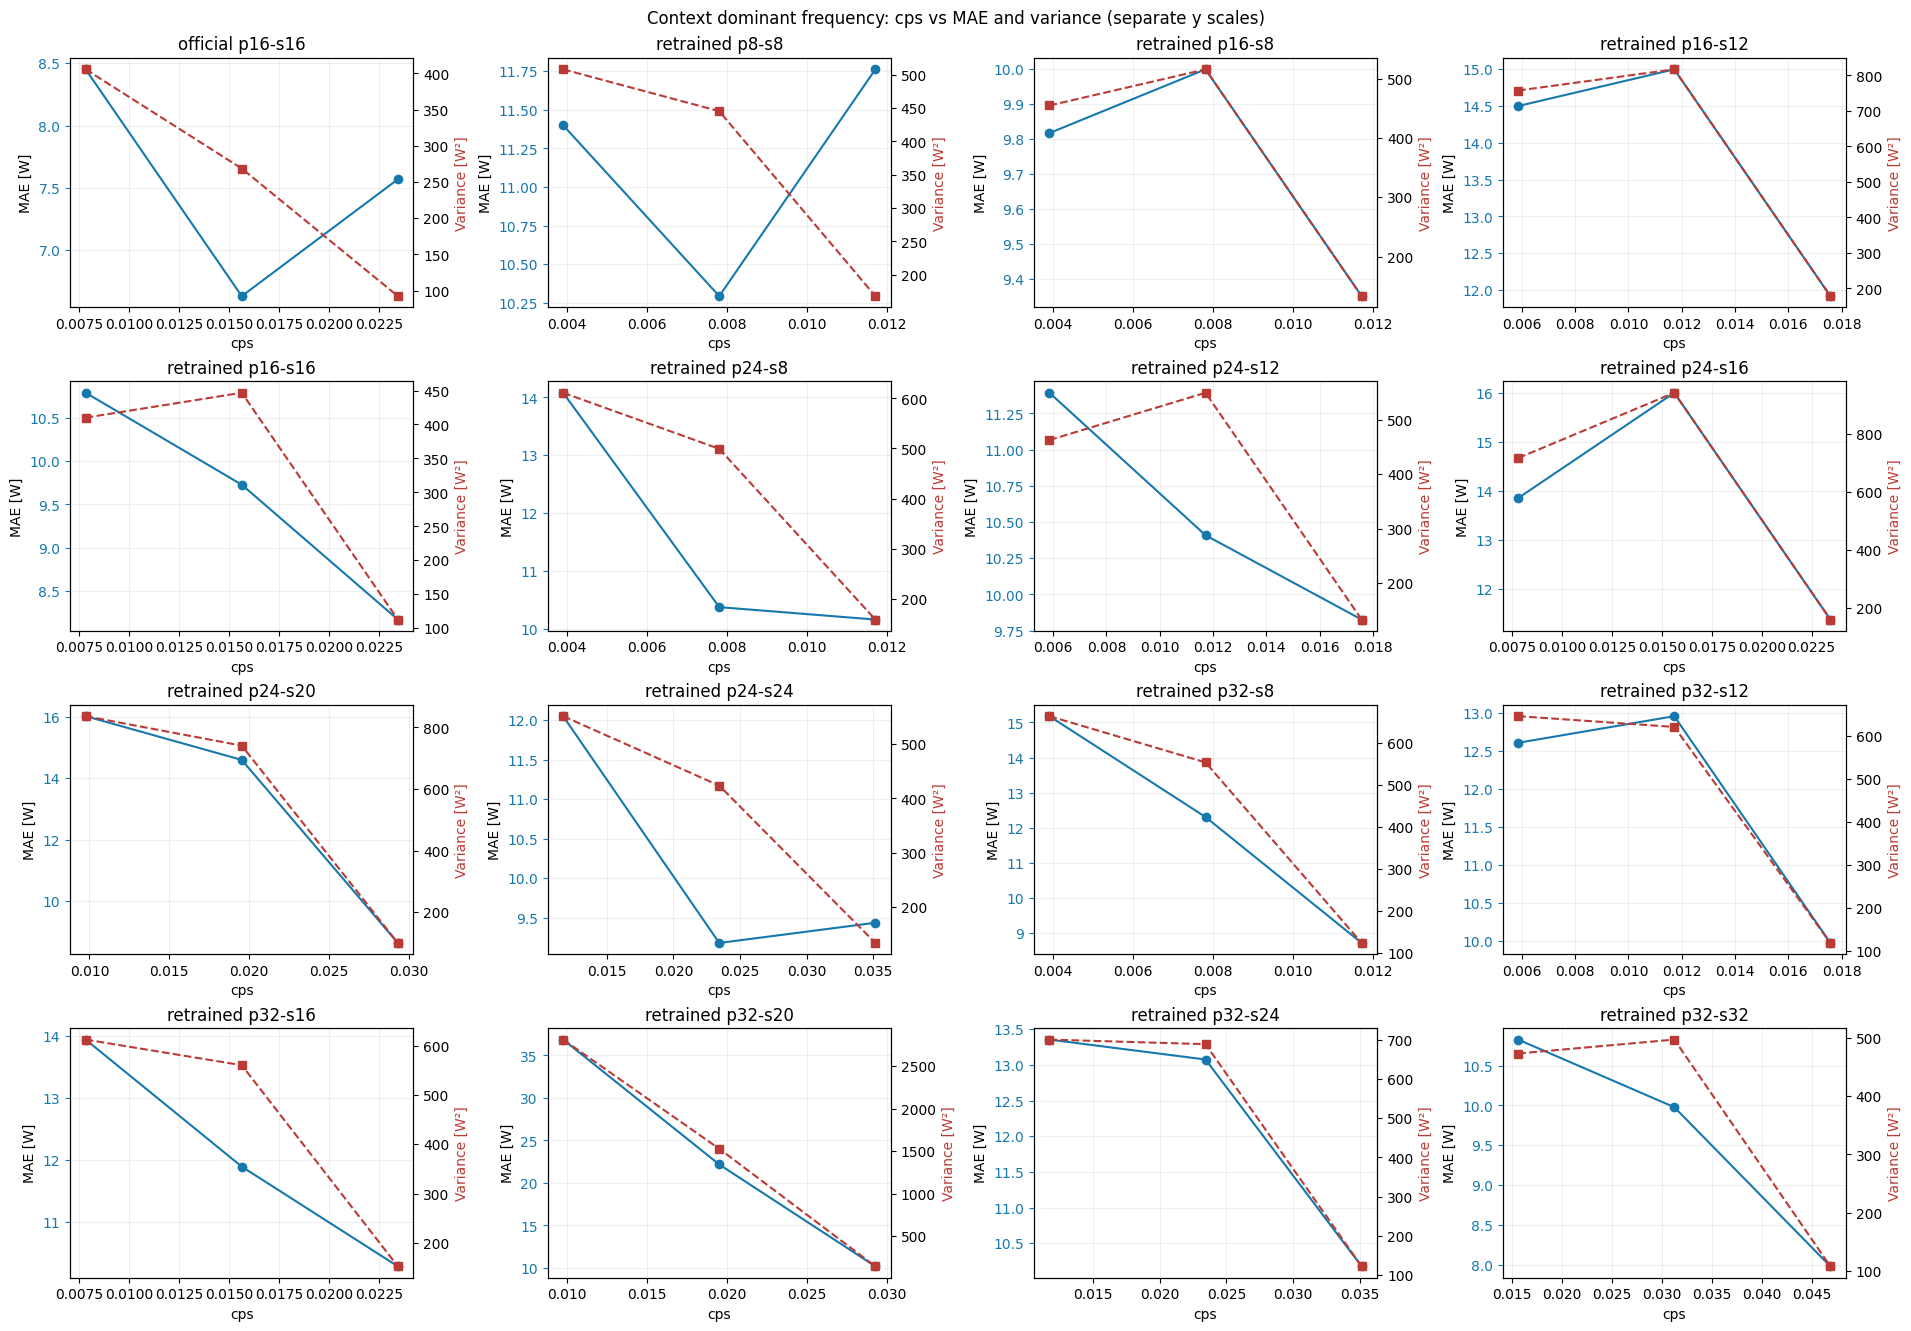
\includegraphics[width=0.85\textwidth]{figures/SOLAR_benchmark_frequency_cps.png}
\caption{Mean absolute error (solid, left axis) and error variance (dashed, right axis) of each model, grouped by the dominant frequency of the context, expressed in cycles per stride of that model's geometry. The three points of each panel hold $108$, $40$ and $2$ windows respectively.}
    \label{fig:solarFreq}
\end{figure}

\FloatBarrier

\subsection{Limits}

The benchmark covers one plant and one year. The published checkpoint was trained with a larger budget and a recipe that is not fully published, possibly on series of this kind, whereas the retrained models follow the published Chronos recipe, so its advantage cannot be attributed to geometry; only the comparison among the retrained models isolates the geometry, and on this series it shows no geometry better than the $P=S=16$ baseline. The zero-filling of night-time minutes is exact, but the zero-filling of long daytime gaps in the context is an assumption.


\end{document}
